%% ====================================================================%%
%%	Sample Driver file for use with uwthesis.sty
%% 	To print this document in the Math Dept, 
%%	do the following:
%%  		latex main
%%		bibtex main
%%		latex main (you may have to do this twice at this point)
%%		dvipr main
%%	To run this sa mple, you will also need the following files
%%		abs.tex, ack.tex,
%%		chap1.tex, chap2.tex, appendix.tex	
%%		thesis.bib	
%% ====================================================================%%
%% 
\documentclass[11pt]{report}
\renewcommand{\familydefault}{\sfdefault}
\usepackage{helvet}
%% If you want to  process the graphics examples in Chap 3 uncomment this line
\usepackage{graphicx}
\usepackage[english]{babel}
\usepackage[backend=bibtex]{biblatex}
\addbibresource{library1.bib}
\usepackage[nottoc]{tocbibind} %Adds "References" to the table of contents


%\usepackage[square, numbers, sort&compress]{natbib}

\usepackage{StyleFiles/mythesis,StyleFiles/tgrind}
\usepackage{fancyhdr}
%% Use this if you only want to do Chap 1 things - basic stuff
%% NOTE: the uwthesis style file should go AFTER all the other packages
%% You may have conflicts if you call the amsthm.sty package after uwthesis.sty

\usepackage{amssymb,StyleFiles/uwthesis}

\graphicspath{
{./Chapters/Introduction/Figures/}
% {./Chapters/Physics/Figures/}
% {./Chapters/FluxCapacitor/Figures/}
% {./Chapters/Concentrator/Figures/}
% {./Chapters/Oscillator/Figures/}
% {./Chapters/TumorCellAdhesion/Figures/}
% {./Chapters/Cardiac/Figures/}
% {./Chapters/RealTimeCM/Figures/}
% {./Chapters/FutureDirections/Figures/}
% {./Appendicies/DropletGeometry/Figures/}
% {./Appendicies/Diffusion/Figures/}
% {./Appendicies/Concentrator/Figures/}
% {./Appendicies/Oscillator/Figures/}
% {./Appendicies/DiffusionValve/Figures/}
% {./Appendicies/Cardiac/Figures/}
% {./Appendicies/RealTimeCM/Figures/}
}

\begin{document}

\title{Open Microfluidic Platforms for Tissue Culture}
\author{Theodorus E. de Groot}

%\inputpicturetrue  % By Jeff McGough. See uuguide and private thesis.sty
%\inputpicturefalse % To NOT produce pictures, uncomment this line


\degree{Doctor of Philosophy}
\dept{Biomedical Engineering}
\thesistype{dissertation}
%% Starts page numbering as i, ii, etc.
\beforepreface
\prefacesection{Abstract}
\input frontmatter/abs 
\prefacesection{Acknowledgements}



\input frontmatter/ack 
%\prefacesection{Papers}
% \input frontmatter/papers
\listoffigures
\listoftables

\afterpreface

%% Include the Chapters
\chapter{Chapter 1: Introduction}\label{Chap:Introduction}





\section{Preface}
Microfluidics are super useful, wow did you know that? I mean they really are the coolest! You can do some really cool stuff with microfluidics when you take off the lid and do open microfluidics. I'm super serious. It's really great. You can do stuff like make Legos or you could do some other stuff like culture cells and do tissue culture in ways that you never thought of before.

\section{Microfluidics for Tissue culture}
Let's talk about tissue culture platforms that used microfluidics because those are really important  n


\section{}
Wow Teddy, you're so smart\cite{Vogler2004a}.





\chapter{Chapter 2: Open Microfluidics Principles}\label{Chap:OpenMicrofluidicsPrinciples}

Knees weak
\chapter{Assays: Cell Adhesion Assay Validation: Tumor-Cell Adhesion to a HUVEC Monolayer}
\label{Chap:TumorCellAdhesion}

\section{Preface}
This work was performed and written in equal collaboration with Edmond Young as represents a manuscript in preparation.

\section{Introduction}
The process of cell adhesion involves physical interactions between cells and the materials in their microenvironment such as extracellular matrices, synthetic biomaterial surfaces, and other cells and is a major topic of interest in areas ranging from fundamental cell biology and pathophysiology \cite{Chen:1997p320,Davies:1995p87} to tissue engineering and regeneration \cite{Nugent:2003p459}. In particular, cell adhesion plays an integral role in inflammation and cancer metastasis where leukocytes and circulating neoplastic cells, respectively, interact with the vascular endothelium in complex adhesion cascades that include tethering, rolling, spreading and endothelial transmigration events \cite{Ley:2007fk,Geiger:2009vn}. The ability to examine and measure the propensity of cells to adhere to the endothelium or other surfaces (engineered or natural) and determine the strength of adhesion is thus critically important to advancing our understanding of the mechanisms related to inflammation and cancer and to the development of tissue engineering strategies in regenerative medicine.

While cell adhesion fundamentally relies on the biophysical and biochemical properties of individual cells \cite{Orsello:2001uq}, many adhesion studies use population-based assays to determine global adhesion characteristics that efficiently reveal important and relevant properties of the cell population \cite{Christ:2010ly}. Population-based adhesion assays typically depend on fluid-flow systems that generate mechanical shear-stress, providing means to promote or challenge adhesion to the substrate on interest in a controlled manner. The most common fluid-flow systems for studying cell adhesion include the parallel-plate flow chamber \cite{GIAVAZZI:1993ty}, radial flow chamber \cite{Goldstein:2002p106}, cone-and-plate viscometer \cite{Jadhav:2001ys}, variable width devices \cite{Heilshorn:2003ly,Usami:1993p603}, and variable-height chambers \cite{Xiao:1996p618}. These systems typically employ steady flow conditions, but they can also be readily modified to accommodate oscillatory or pulsatile flow conditions for studies in shear-mediated atherosclerosis and cardiovascular pathobiology \cite{KU:1985uq,Chappell:1998fk}. Depending on the purpose of the study and availability of resources, flow systems can be operated under various schemes or protocols to produce different types of adhesion assays. For example, flow-rate\slash shear-stress can either be increased or decreased in a stepwise fashion to assay the gradual detachment or attachment of cells, respectively. Furthermore, shear-stress ranges can be expanded, or the number of steps in the ramping scheme can be increased to yield a more continuous scheme with better resolution for detecting adhesion events than more discrete protocols. Although fluid-flow systems have become indispensable tools in biological research, these systems have significant drawbacks due to their large scale, complex setup, and need for large volumes of medium and cell suspension to maintain flow. 

Recently, a number of microfluidic systems have been developed for cell adhesion and shear-flow assays \cite{Lu:2004ys,Gutierrez:2007p290,Plouffe:2007p274,Young:2007ml}, taking advantage of microfabrication techniques to create systems that can increase throughput, handle reduced fluid volumes, and improve spatiotemporal control of \invitro\ microenvironments \cite{Young:2010p286,Young:2010uq}. While these microscale flow systems have shown improvements over their macroscale counterparts and have overcome some of the main drawbacks of previous systems, the majority of microfluidic systems continue to require complex ``world-to-chip'' interfacing \cite{Fredrickson:2004ve} that limits their potential for widespread adoption in biology labs, particularly in clinical and translational research applications where limited patient-derived cell and tissue samples may be significantly depleted by excessive tubing and large dead volumes. 

We have developed a novel microscale system for conducting oscillatory, shear adhesion assays that employs passive-pumping principles to eliminate cumbersome interconnects and unnecessary tubes and dead volume. The system, described in detail below, enables pipette-based loading and treatments, is easily amenable to complex microscale geometries, and can be dynamically controlled to offer various oscillatory waveforms for cardiovascular applications. Most importantly, this microscale system offers analysis of the adherence of a small and defined population of cells in a manner that cannot be achieved with existing systems, thus enabling studies of limited cell samples such as those acquired from a clinical setting. These capabilities, coupled with a custom information-rich readout, allow this system to be applied to a wide range of biological experiments. To illustrate the potential of this system and custom readout, we developed an attachment-based adhesion assay that utilizes a decreasing log-sweep of shear-stress and differential image analysis of image-streams to quantify the process of adhesion for an entire population of interest. We used the integrated system to study adhesion of three different cancer cell-lines on activated and non-activated endothelial monolayers. Results demonstrate the ability of this approach to provide new insights into the heterogeneity of cell populations and adhesion mechanisms.

\section{Results and Discussion}

\subsection{System Design and Operation}

Our main objective was to design, test, and implement a passive-pumping-based oscillatory flow system for an array of microchannels in order to extend oscillatory modes of shear flow to pipette friendly systems.  Passive-pumping has been used previously in various applications, and has been described in detail elsewhere \cite{Berthier:2007mi,Meyvantsson:2008,Walker:2004ov}. Briefly, passive-pumping leverages surface tension to pump fluid from small droplets to larger droplets based on Laplace's law (Figure \ref{figure:schematic}A). We fabricated a simple one-input-one-output straight microchannel where one port is smaller than the other to facilitate passive-pumping of cell suspensions, media, and reagents. To generate oscillatory flow, we further designed and fabricated a diaphragm from polydimethylsiloxane (PDMS) that was positioned over the larger outlet port and reversibly sealed to the top of the PDMS microchannel. The diaphragm was actuated using a piezoelectric cantilever which bends in response to a voltage signal. The actuator was retrofitted with an adjustable cap screw to provide a single point of contact between the actuator and diaphragm (Figure \ref{figure:schematic}B). Voltage signals were produced using a function generator and passed through an amplifier to the actuator to tunably control displacement of the cap screw tip. The resulting deflections of the diaphragm induce pressure changes within the sealed air chamber below the diaphragm to drive oscillatory flow within the microchannel. The ports act as reservoirs for volume fluctuations with the exposed port providing pipette access to deliver treatments or cell suspension.

\begin{figure}[ht] %DONE
\centering
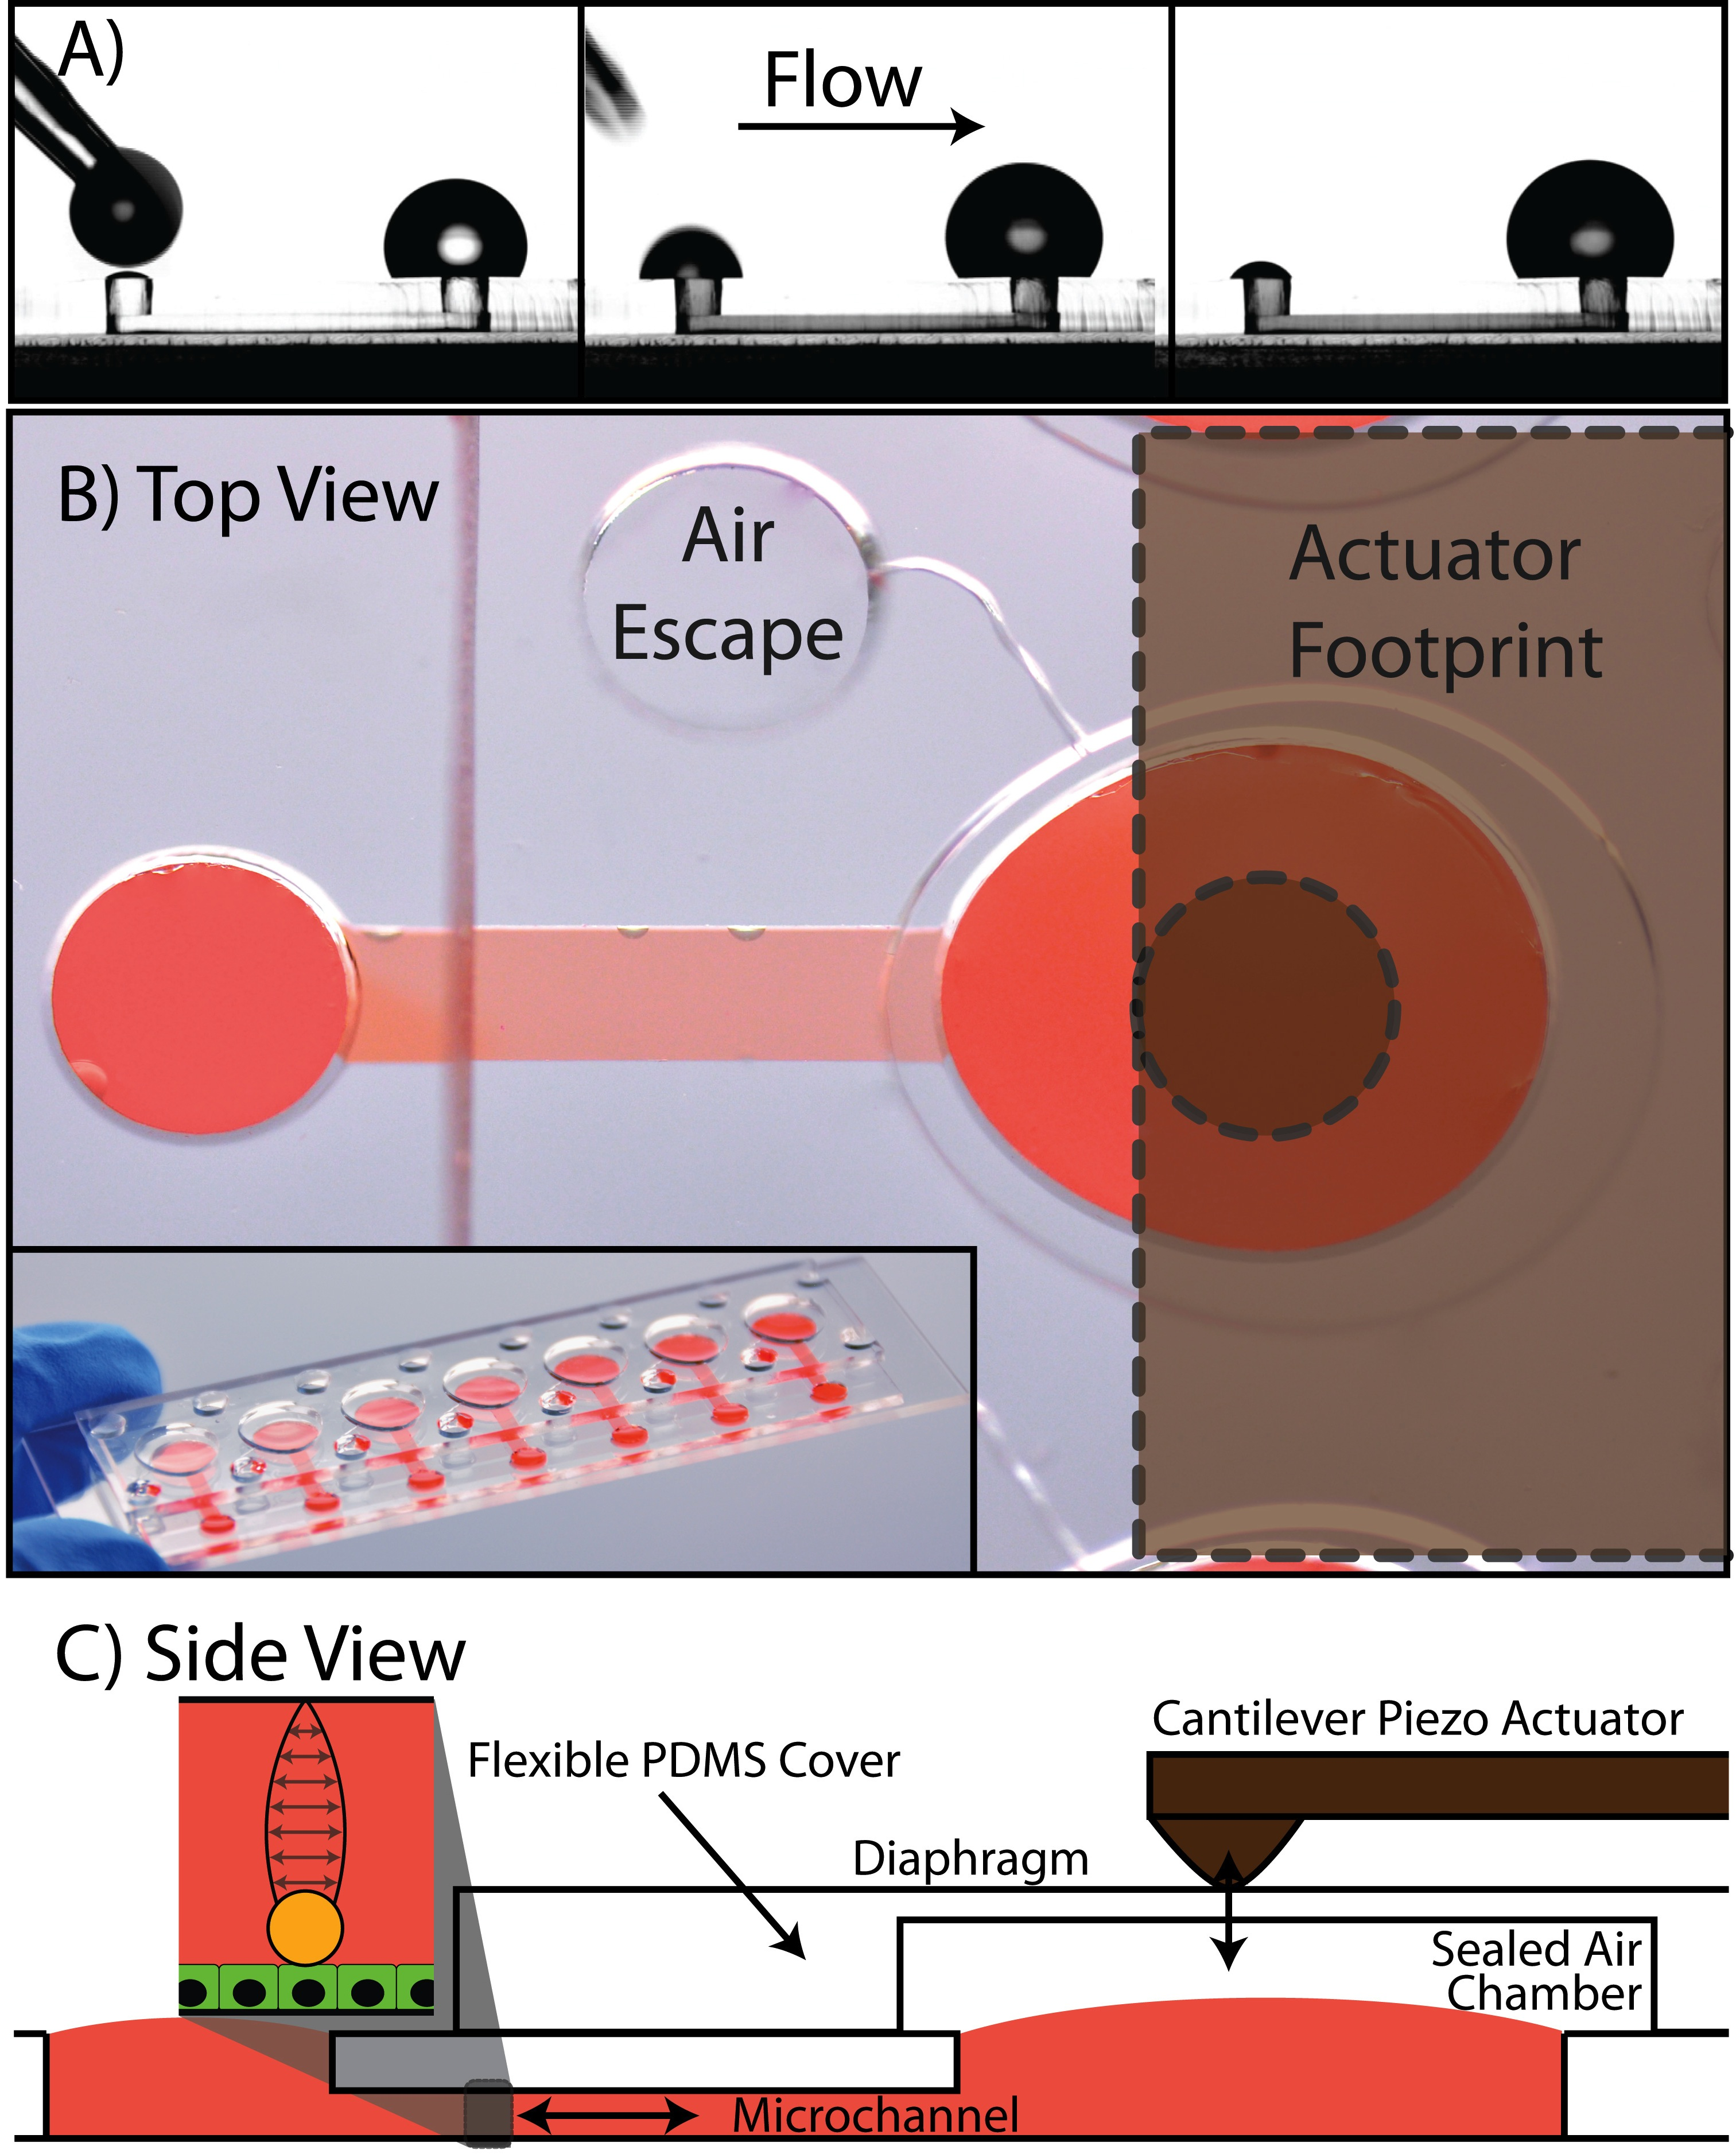
\includegraphics[width=3.5in]{OscillatoryDiagram4.jpg}
\caption{\textbf{Oscillatory flow device}. (A) Side images of passive pumping via dispensed droplets. (B) Top view of microchannel and diaphragm assembly. Inset shows 7 x 1 array of microchannels on a single microscope slide. (C) Side view of setup. Cantilever piezoelectric actuator deflects diaphragm according to applied voltage signals. At low frequency and moderate amplitude, this creates a volume change in the air cavity and displaces fluid in the channel. Oscillatory shear-stresses may be generated with this approach, allowing it to be used for various cell adhesion studies.}
\label{figure:schematic}
\end{figure}

The dimensions of the straight microchannel mimic the dimensions of a conventional parallel-plate flow chamber while the microchannel ports provide the ability to load and treat cells via pipette. The use of microfabrication techniques will allow us to rapidly explore more complex designs in the future. The footprint of the device provides a modest increase in throughput, i.e., up to seven microchannels per array during one microscope acquisition session, but perhaps more importantly, the microchannels were independently addressable. Maintaining separation ensures that each endothelial monolayer is cultured, activated, and\slash or mechanically stimulated as independent biological samples without adverse cross-talk, as is the case in many multiplexed microfluidic systems. In co-culture adhesion studies, this property has the potential for an even larger impact: the system can test limited cell samples, such as those acquired from clinical patients, as demonstrated by our use of $\sim 10^4$ cells per channel. This is a relatively small amount of cells compared to $\sim 10^6$ to $10^7$ cells typically needed for large-scale (mL) continuous flow in parallel-plate flow chambers. We envision that the system can be scaled if necessary to take even fewer cells ($10^2$ or $10^3$ cells), with only minor modifications to microchannel dimensions.

The oscillatory flow methods used here also have potential utility in other biological applications such as cardiovascular and bone mechanobiology, where oscillatory shear-stress has been implicated in important regulatory functions. Macroscale oscillatory flow systems have already been accepted into the laboratory setting while microscale oscillatory systems (and recirculatory systems in general) have also begun to appear \cite{Song:2005p157,Shao:2009p534}; however, the current design is the first oscillatory system to employ passive-pumping, thus combining the advantages of microscale approaches with simple pipette-based operation that obviate the need for tubing that inherently leads to excess dead volume.

The most innovative features of the demonstrated method are the integrated use of the piezoelectric actuator-PDMS membrane, and the development of a unique cell adhesion readout that has potential to offer new biological insights into cell adhesion phenomena. We leveraged the elastic properties of PDMS to create a sealed air chamber and diaphragm with negligible damping effects below 30 Hz and moderate amplitudes. However, oscillatory flow in a microchannel of these dimensions produces non-linear shear-stress response above 5 Hz. Above 5 Hz, the flow profile becomes non-parabolic. Above 30 Hz, the compliance of the air chamber results in significant attenuation of shear-stress. However, a property of laminar flow (steady and pulsatile) is that shear-stress at a given frequency is always linear to the pressure gradient. Clearance between the diaphragm and fluid in the port also limits actuator amplitudes. However, only 30 \textmu m of motion is required to produce the maximum shear-stress used in this study. As mentioned earlier, the microchannel ports act as reservoirs for oscillatory fluid exchange and thus limit the total volume that can be exchanged between the ports per cycle. The adhesion studies to date have been done in the low frequency regime where damping is insignificant leading to a linear relationship between frequency and shear-stress.

\subsection{Adhesion Assay via Image Differencing}

\paragraph{Measurement of Attachment \vs\ Detachment.}The use of a piezoelectric actuator enables the use of a wide variety of signal waveforms and flexible control of the shear-stress protocol. This capability allowed us to develop an 8-minute adhesion assay that samples a large range of frequencies at high resolution using a logarithmic sweep that spans two orders of magnitude (2 Hz to 100 mHz). Thus, this system provides similar resolution to that presented recently by \cite{Christophis:2010fk}. However, in contrast to Christophis \etal\ and other assays that ramp up shear-stress to detect detachment events, we have employed an inverse strategy where cells are initially prevented from adhering by starting at a relatively high shear-stress and then gradually \emph{reducing} shear-stress in order to monitor the \emph{attachment} events instead of \emph{detachment}.

\paragraph{Oscillatory \vs\ Flow-Through Methodologies}Although both oscillatory and flow-through devices can be used to study both attachment and detachment, the use of oscillatory flow fundamentally changes the readout of an attachment assay compared to flow-through devices and provides new insights into adhesion properties that have not been previously obtained. The \emph{attachment} readout of the oscillatory adhesion assay is identical to the \emph{detachment} readout reported by Christophis \etal. In the case of Christophis \etal\, the population of interest is completely defined prior to detachment, enabling them to present detachment results over a range of shear-stresses in terms of ``\% of the entire population of interest''. In doing so, they are able to directly measure the shape of the population distribution with respect to detachment shear-stress. The ability to measure the shape of the population distribution can provide important insight into the mechanisms of adhesion. In our case, the population of interest can also be defined as those cells that are initially in the field-of-view. The oscillatory nature of the flow allows us to monitor this population of interest over time for different levels of shear-stress to report the number of adhered cells as a \% of the entire population at various shear-stresses, thereby directly measuring the shape of the population distribution as well. This is different from other attachment assays that used flow-through or recirculation devices. When flow-through devices (\eg, the Christophis \etal\ device) are used in ``attachment-mode'' it becomes more difficult to define what an entire population is and makes it much more challenging to elucidate the shape of the population distribution. Thus, it is the oscillatory nature of the flow that enables a direct measurement of population distributions for attachment assays.

A previous study by Wang \etal\ used pulsing flow to study cell attachment and leveraged the ability to follow a single cell over time to examine individual attachment events; however, shear-stress in the system is uncharacterized and the readout was not extended to provide information regarding the distribution of the population \cite{Wang:2009kl}. The embodiment also differs significantly from that reported here given the use of tubes and a mechanical pumping mechanism with limited flexibility for defining complex flow patterns. Also, the study used image streams and image differencing to obtain measurements of \emph{cell motion} which were then normalized using knowledge of cell densities and suspension volumes to compare relative amounts of adhesion between two different cell populations at a given shear-stress. Here, a fully automated algorithm uses image difference information to directly measure the percent of cells adhered for an entire population over a range of shear-stresses.

\paragraph{Image Analysis: Preprocessing.}The percent of adhered cells is determined using phase-contrast microscopy. The data set for each channel consists of 41 image streams, each containing 25-170 images depending on the length of time needed to acquire 1-2 cycles of cell motion. The background is subtracted from all the images in the data set. The image used for background subtraction is determined from the first stream of images. In phase contrast using low magnification (2X), the cells appear brighter than the background. Thus, a stack projection is performed on the first stream to determine the minimum intensity for each pixel over time, removing any brighter moving objects (\ie, suspended cells) from the resulting background image. Thus, the background subtracted images in the data set are greatly enhanced to show suspended cells that were added to the channel. By using the same background image to perform all background subtraction for a given channel, any suspeded cells that adhere at a later time-point will still show up as being bright. An Otsu automatic thresholding routine is used to threshold the enhanced images to produce binary images with cells appearing white and background black. The background subtraction process produces stark contrast between the cells and background to make the automatic thresholding routine very robust. A single region of interest (ROI) is then chosen and applied to all images of the data set to restrict analysis from considering portions of the image where no cells exist and where shear-stress is uniform. Given the channel dimensions used in this study, the center 80\% of the channel width exhibits uniform shear-stress and is chosen using the ROI. All subsequent analysis is limited to this ROI.
 
\paragraph{Image Analysis: Quantifying the Percent of Adhered Cells.}Fig \ref{Chap:TumorCellAdhesion:fig:differencing} shows an idealized version of the black and white image streams that result from preprocessing and helps to describe the algorithm used to determine the percent of cells adhered to the substrate. In any given frame of a stream, there can be adhered (A) and non-adhered (NA) cells. In a different frame of the same series, non-adhered cells show up in a different location whereas adhered cells remain in the same spot. Thus, if we take the absolute difference of these two frames the non-adhered cell will show up twice whereas the adhered cell will show up once. Depending on the frames that are chosen, the impressions of the non-adhered cell may partially overlap.

\begin{figure}[!bt]
\centering
\includegraphics[width=6in]{ImageDifferencing.pdf}
\caption{\textbf{Image differencing algorithm}. $F_{n}$ refers to the $n^{th}$ frame of a time-series of images. $F_{n+\Delta n}$ refers an image taken $\Delta n$ frames after $F_{n}$. NA refers to a cell that is \underline{n}ot \underline{a}dhered where as A refers to a cell that is \underline{a}dhered.}
\label{Chap:TumorCellAdhesion:fig:differencing}
\end{figure}

If the impressions do not overlap then Eq \ref{Chap:TumorCellAdhesion:equ:percentAdhered} can be used to predict the percent of cells adhered where $F_{i}$ represents the integrated intensity of the $i^{th}$ binary image. For each stream the reference frame $F_{n}$ is chosen as the frame which exhibits the most average intensity over the course of the stream. The quantity $\left| F_{n}-F_{n+\Delta n}\right|$ is then calculated for all other images while holding $F_{n}$ constant. Partial overlap reduces the value of $\left| F_{n}-F_{n+\Delta n}\right|$ and is expected to occur less than 30\% of the time given our number of frames and minimum cell amplitudes. Therefore the top 5\% of these values are averaged to potentially reduce noise in determining a final value for the numerator of Eq \ref{Chap:TumorCellAdhesion:equ:percentAdhered}. This number is proportional to twice the number of non-adhered cells whereas $F_{n}$ is proportional to the number of total cells, thus arriving at Eq \ref{Chap:TumorCellAdhesion:equ:percentAdhered} for the percent of adhered cells. This process is repeated for each of 41 streams in the data set for each channel to produce a plot of `\% of Population Adhered' \vs\ `Shear-Stress'. It is possible that if oscillation and image acquisition were synchronized, image streams would no longer be necessary as a good choice for $F_{n}$ and $F_{n+\Delta N}$ can be predicted based on the sinusoidal nature of the oscillation.

\begin{equation}
\textrm{\% of Pop. Adhered} = 1 - \frac{\left| F_{n}-F_{n+\Delta n}\right|}{2 \, F_{n}}
\label{Chap:TumorCellAdhesion:equ:percentAdhered}
\end{equation}

\paragraph{Batch Processing.}The image filtering and analysis is completely automated using custom software called Je'Xperiment, developed by Jay Warrick and Erwin Berthier at the University of Wisconsin Madison. The software is used to database the images and perform batch processing of the custom algorithm. One array of 7 channels produces approximately 10-15 gigabytes of data. The primary time constraint of the analysis is thus the time it takes to read and write the images to a hard drive or server ($\sim$ 5 hours total). However, Je'Xperiment allows one to obtain results with less than 10 minutes of time actually invested by the user at the computer workstation.

\paragraph{Interpretation of Results.}Fig \ref{Chap:TumorCellAdhesion:fig:logNorm} illustrates the shape of the resulting adhesion plot and the log-normal cumulative distribution function (LNcdf) used to fit the data. The LNcdf (Eq \ref{Chap:TumorCellAdhesion:equ:LNcdf}) has two parameters, $\mu$ and $\sigma$, which are obtained from the curve fit. The quantity $e^{\mu}$ represents the median shear-stress of the population, $\tau_{50}$, whereas $\sigma$ indicates the spread, measured in orders of magnitude, of the data surrounding the median. This interpretation is different than a normal distribution where $\sigma$ gives an indication of absolute spread about the mean.

\begin{figure}[!t]
\centering
\includegraphics[width=3.5in]{TheoryPlot.pdf}
\caption{\textbf{Log-normal cumulative distribution function}.}
\label{Chap:TumorCellAdhesion:fig:logNorm}
\end{figure}

\begin{equation}
\textrm{LNcdf($x$,$\mu$,$\sigma$)} = \frac{1}{2} + \frac{1}{2}\textrm{erf}\left[ \frac{\ln{x} - \mu}{\sqrt{2 \sigma^{2}}}\right] 
\label{Chap:TumorCellAdhesion:equ:LNcdf}
\end{equation}

Interpretation of changes in the median are fairly straight forward but changes in $\sigma$ are less intuitive. For example, assume there is a cell type and a substrate that interact via one type of molecule with a median shear-stress of 1 Pa and has a $\sigma$ of 1 indicating that 97.89\% of all cells in the population adhere at a shear-stress between 0.1 and 10 Pa. In this idealized scenario, if the substrate is changed such that only 1/10$^{th}$ the original amount of adhesion ligand is presented to the cells, one would expect the median shear-stress to drop to roughly 0.1 Pa given that the number of anchor points per cell is lowered accordingly. Since each portion of the population would fall under this argument, shear-stress data would be predicted to simply shift while keeping $\sigma$ the same. That is to say, the new median shear-stress would be 0.1 Pa with 97.89\% of the population falling between 0.01 and 1 Pa.

On the other hand, what if the median does not change and $\sigma$ does? Given $\sigma$ is a measure of the heterogeneity of the interaction between the cells and substrate, a change in $\sigma$ indicates that the type of mechanism mediating adhesion (\ie\ the involvement of specific molecules or physical forces) has changed or has become more or less heterogeneous. However, it is more likely that multiple molecules or mechanisms mediate adhesion and contribute to an overall perceived heterogeneity. In this situation, if the influence of one of those contributing mechanisms were to be heightened, the value of $\sigma$ would change as well. If a single population has two dominant mechanisms of adhesion, it would result in the multiplication of two characteristic LNcdfs. On the other hand, if there are \emph{two} distinct populations, the result would be the renormalized addition of the two characteristic LNcdfs.

Thus, changes in $\sigma$ are associated with changes in the heterogeneity of the underlying mechanism, whereas changes in the median indicate changes in the strength or number of the interactions.

\subsection{Cancer cell adhesion}
Having defined the oscillatory attachment assay methodology, readout, and method of data interpretation; biological experiments are performed to characterize the sensitivity and repeatability of the assay for detecting physiologically relevant changes in adhesion interactions. We tested adhesion of three established cell lines derived from distinct types of cancer, including prostate (PC3-MM2), breast (MDA-MB231), and multiple myeloma (RPMI8226).  Studies on the adhesiveness, invasiveness and metastatic potential of these cell lines have shown that PC3-MM2 cells are particularly invasive among PC3 family of sublines \cite{Daja:2003rr}, and that PC3 sublines are highly variable in adhesiveness \cite{Dimitroff:2004bh}. MDA-MB231 cells are also highly invasive among breast cancer cell lines \cite{TOZEREN:1995wd,Lee:2003kx}, but are known to adhere to activated endothelium only in the absence of shear-stress $> 0.5$ dyn/cm$^2$ \cite{TOZEREN:1995wd}. In contrast to prostate and breast cancers, the adhesiveness and invasiveness of cells of multiple myeloma (MM) origin has been studied to a much lesser extent. Reports of MM cell adhesion that are available seem to suggest that adhesion to (bone marrow) endothelium is mediated by various molecules other than E-selectin \cite{Okada:1995ys,Broek:2008p301,Katz:2010uq}. Thus, we expected that PC3-MM2 and MDA-MB231 cells would exhibit more adhesive phenotypes, while RPMI8226 would likely show less adhesion to the endothelial monolayers.

We performed independent LNcdf curve fits for each condition, extracted the fitted $\tau_{50}$ and $\sigma$ values and compared results between activated and non-activated endothelium as well as across the different cell types. Fig \ref{Chap:TumorCellAdheison:fig:examples} shows examples of data and LNcdf fits for each cell type on activated and non-activated endothelium.

\begin{figure}[ht] %DONE
\centering
\begin{tabular}{cc}
A) PC3-MM2 & B) RPMI8226 \cr
\includegraphics[width=2.5in]{ExamplePC3.pdf} &\includegraphics[width=2.5in]{ExampleRPMI.pdf} \cr
C) MDA-231 & \cr
\includegraphics[width=2.5in]{ExampleMDA.pdf}
\end{tabular}
\caption{\textbf{Example adhesion curves for each condition}. Each pair of curves represents a adhesion measured in two channels on the same day. (blue) Non-activated endothelium. (red) Activated endothelium. }
\label{Chap:TumorCellAdheison:fig:examples}
\end{figure}

We observed statistically significant increases in $\tau_{50}$ (the critical shear-stress) between activated and non-activated endothelial surfaces for all cell types, including, surprisingly, RPMI8226 cells (Figure \ref{Chap:TumorCellAdhesion:fig:summaryGraphs}A). Comparing non-activated endothelium cases alone, both MDA-MB231 and PC3-MM2 cells exhibited significantly higher values of $\tau_{50}$ than RPMI8226 cells; this was also true for the activated endothelium cases alone, where MDA-MB231 and PC3-MM2 cells had higher $\tau_{50}$ than RPMI8226 cells (Figure \ref{Chap:TumorCellAdhesion:fig:summaryGraphs}A). Interestingly, when the \emph{ratio} between activated and non-activated $\tau_{50}$ values were calculated and compared, no difference was found between cell types (Figure \ref{Chap:TumorCellAdhesion:fig:summaryGraphs}B), suggesting that the effect of IL-1$\beta$ induction on adhesion was consistent across cell types. Thus, MDA-MB231 and PC3-MM2 cells were likely more adhesive than RPMI8226 cells because of intrinsic differences in cell surface properties, which were amplified for all cell types in the presence of E-selectin. This appeared to be consistent with the literature cited above.

\begin{figure}[!tb] %DONE
\centering
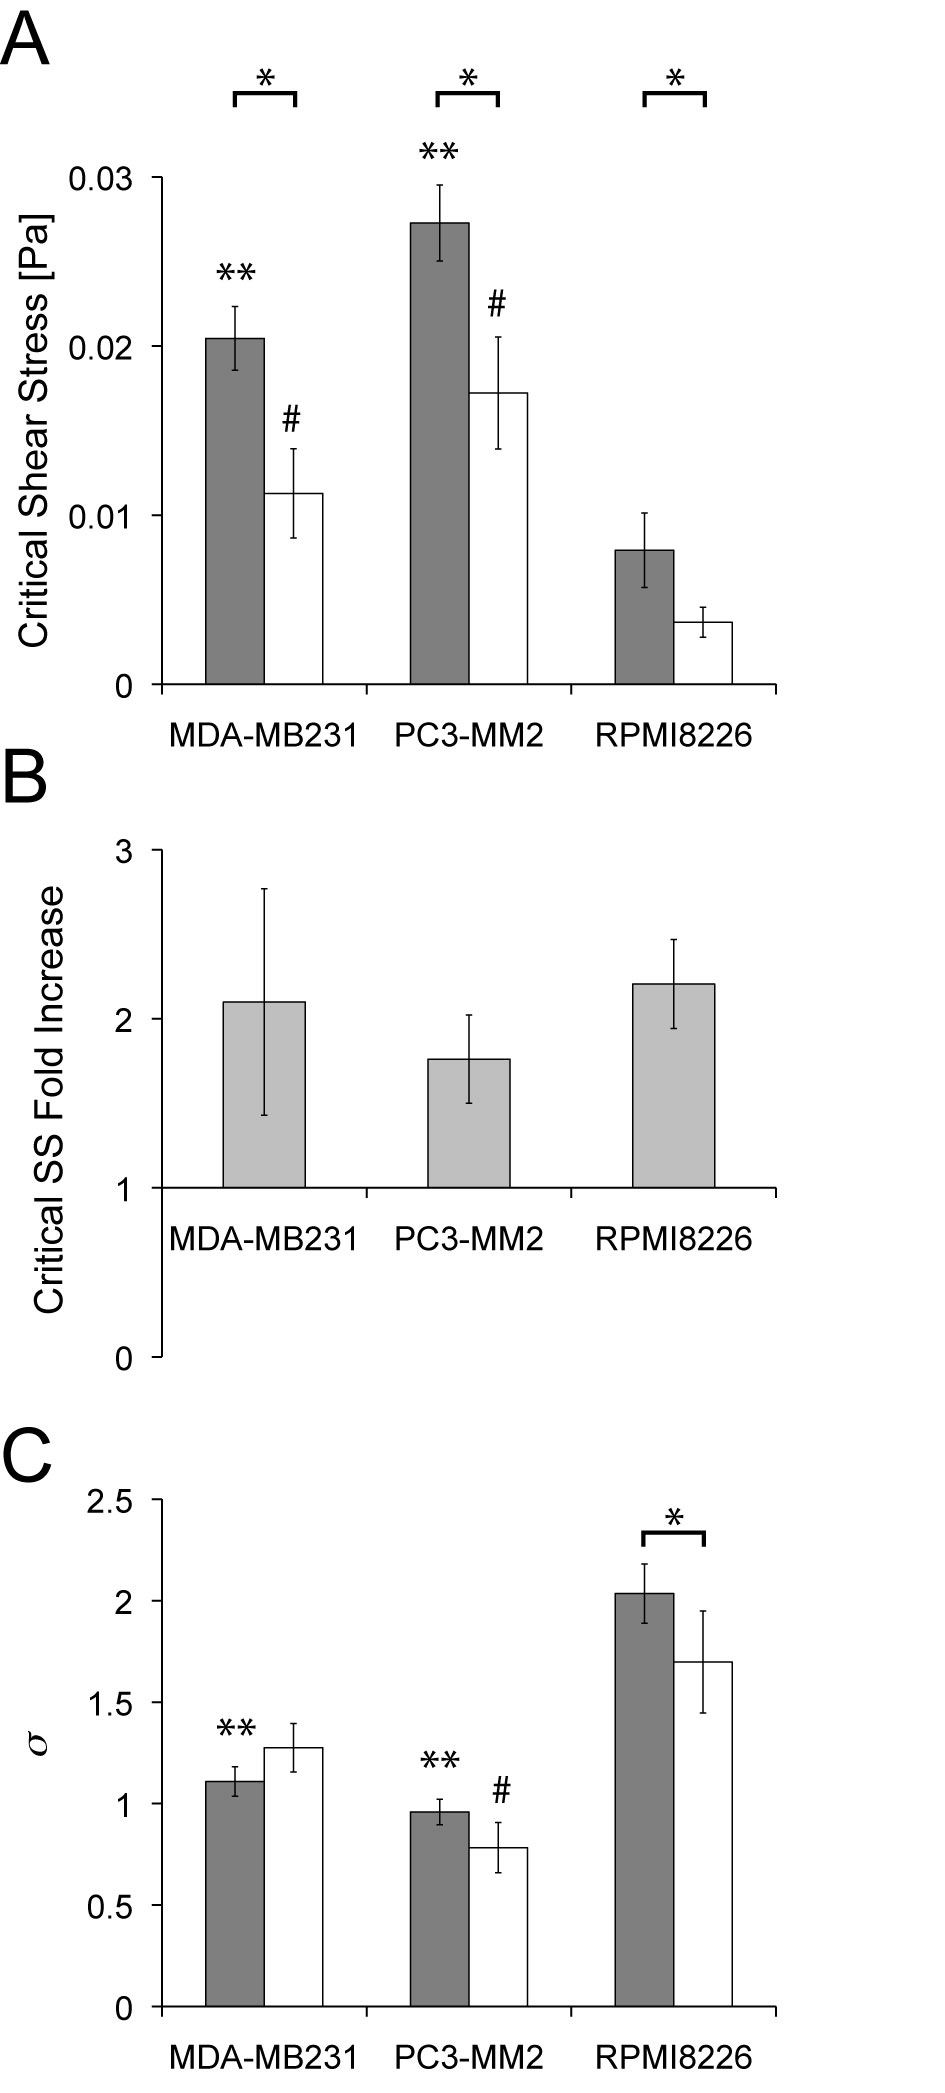
\includegraphics[height=6in]{Figure_FinalGraphs.jpg}
\caption{\textbf{Comparison of adhesion to a HUVEC monolayer}. (A) Average critical shear-stress on activated (gray bars) and non-activated (white bars) endothelium. (B) Average fold increase in critical shear-stress. (C) Average $\sigma$ of lognormal distribution on activated (gray bars) and non-activated (white bars) endothelium. $\ast: P < 0.05$ for combined block multiple experiments between activated and non-activated endothelium for given cell type. $\ast\ast: P < 0.05$ compared to RPMI8226 on activated endothelium.  $\#: P < 0.05$ compared to RPMI8226 non-activated endothelium.}
\label{Chap:TumorCellAdhesion:fig:summaryGraphs}
\end{figure}

Fitted values of $\sigma$ were also compared between non-activated and activated endothelium groups and  across cell types. No statistically significant differences were found between activated and non-activated endothelium conditions for comparisons within each cell type (Figure \ref{Chap:TumorCellAdhesion:fig:summaryGraphs}C). However, $\sigma$ values for RPMI8226 cells were significantly higher than those for PC3-MM2 and MDA-MB231 for both activated and non-activated endothelium groups. These data suggested that $\sigma$, which represents the heterogeneity in cell adhesion of the population, was not influenced by endothelial activation, but only by intrinsic differences between cells. 

Collectively, the pair of fitted parameters $\tau_{50}$ and $\sigma$ have revealed expected yet nevertheless interesting similarities and differences between the cancer cell types, which can be interpreted as follows. No difference in the heterogeneity of the metastatic breast and prostate cancer cell line adhesion could be observed and this heterogeneity did not change significantly upon activation of the endothelium. That is to say, although endothelial activation enhanced adhesion for these two cell types, the level of enhancement was consistent across all individual cells within the population (i.e., no change in spread in the LNcdf was observed), and consistent across cell types (\ie, no significant change in the fold-increase of $\tau_{50}$ was observed either). RPMI8226 cells were similarly affected by endothelial activation, but in comparison to PC3-MM2 and MDA-MB231 cells, RPMI8226 cells were much less adherent and displayed much more heterogeneity in the population. This heterogeneity is potentially related to its low adherence, since loose adhesion from non-specific interactions is likely to yield low $\tau_{50}$ and high $\sigma$. 

\section{Conclusion}
A novel approach for examining cell attachment has been presented that integrates a unique method for producing oscillatory flow, high resolution sweep of shear-stress, fully automated image analysis algorithm, and comprehensive examination of population heterogeneity. The sensitivity and repeatability of the method was validated by confirming an increase in adhesion of three different tumor cell lines representing 3 different cancers to a HUVEC monolayer upon activation of the monolayer using IL-1$\beta$. Unique insight into population heterogeneity was enabled by the use of oscillatory flow. The use of oscillatory flow also enabled the use of passive-pumping to allow samples to be loaded and treated using a pipette. Thus, the platform enables complete separation of microchannels to ensure independence of each data point acquired in the array. Taken together, the method presented here offers new insight into cell adhesion, represents a significant advance to the study of cell attachment, and has the potential to advance our understanding of adhesion in areas such as cancer metastasis, inflammation, and regenerative medicine.

\section{Materials and Methods}

\subsection{Cell Culture}

Human umbilical vein endothelial cells (HUVECs) were purchased from Lonza (Walkersville, MD), and regularly cultured on tissue culture-treated flasks pre-coated with 1.5 $\mu$g/cm$^2$ of bovine plasma fibronectin (FN) (Sigma-Aldrich, St. Louis, MO). HUVECs were maintained in EGM BulletKit media (CC-3124, Lonza) consisting of EBM-2 basal medium supplemented with 2\% fetal bovine serum (FBS), bovine brain extract with heparin, hEGF, hydrocortisone, and gentamicin/Amphotericin B. HUVECs were fed every other day, passaged every 3-4 days at 90\% confluence, and only passages 4-6 were used in microchannel experiments. 

To prepare HUVEC monolayers for adhesion tests, microchannels were first primed with 30 $\mu$L PBS followed by 20 $\mu$L FN at 100 $\mu$g/mL concentration. Microchannels were incubated at 37 deg C for 1 h in humidified trays to allow FN adsorption to the microchannel walls. After incubation, FN was replaced twice with 40 $\mu$L HUVEC media further supplemented with 10 mM HEPES. HUVECs were seeded at 3000 cells/$\mu$L $\times$ 6 $\mu$L per microchannel, and allowed to adhere and culture overnight (12 h). HUVEC microscale cultures were either used on the same day for adhesion tests if confluent, or maintained for an additional day to reach full confluence. Activated HUVEC monolayers in microchannels were induced with 10 $\mu$g/mL interleukin-1$\beta$ (IL-1$\beta$) for 4 h before adhesion tests.

Three different human cancer cell lines were used in adhesion tests to compare adhesion strengths on activated versus non-activated endothelium. MDA-MB231 cells (mammary gland epithelial) were maintained in DMEM with 4.5 g/L glucose supplemented with 10\% FBS and 1\% penicillin/streptomycin (P/S). PC-3 MM2 cells (metastatic prostate) were maintained in RPMI1640 with L-glutamine, 10\% FBS, 1\% penicillin/streptomycin (P/S), and 10 mM HEPES. RPMI8226 cells (multiple myeloma in bone marrow) were maintained in DMEM with 4.5 g/L glucose supplemented with 10\% FBS, 1\% P/S, and 10 mM HEPES.  MDA-MB231 and PC3-MM2 cells were fed every other day and passaged every 3-4 days depending on confluence. RPMI8226 cells were passaged every 3 days. All cell lines were resuspended at 1000-1500 cells/$\mu$L, and 7.5 $\mu$L of cell suspension was dispensed into each microchannel. Thus, each microchannel contained approx. 7,500 to 12,000 cells.

\subsection{Immunostaining and HUVEC activation}

Immunostaining was performed to verify upregulation of E-selectin upon activation using IL-1$\beta$. Fig \ref{Chap:TumorCellAdhesion:fig:staining} shows that E-selectin upregulation was robust for all concentrations tested while the control showed basal levels. Acquisition parameters were identical and images were treated uniformly.

\begin{figure}[!ht]
\centering
\includegraphics[width=3.5in]{StainingImages.pdf}
\caption{\textbf{HUVEC staining for E-selectin}. Concentration of IL-1$\beta$ is indicated in the corner of each image.}
\label{Chap:TumorCellAdhesion:fig:staining}
\end{figure}


\subsection{Image Capture and Analysis}

Prior to data acquisition, a calibration procedure described in Chapter \ref{Chap:Oscillator} was used to measure the initial shear stress of the system at 140 mV piezo voltage and 2 Hz sinusoidal oscillation frequency. The actuator was perturbed by gentle tapping to redistribute cells within the field of view that moved due to the calibration procedure. After waiting 30 seconds for cells to settle, the acquisition protocol was started.

Data acquisition consists of 41 stream acquisitions. The first 5 are to be acquired at 2 Hz. At the start of the sixth stream, a descending log frequency sweep is begun that lasts for 500 s and ends at 0.1 Hz. The first six datapoints obtained at a frequency of 2 Hz are used to normalize each curve. The average of those six measurements is forced to a value of one resulting in a proportional adjustment of all other values.

MetaMorph was used to acquire the image streams at specified intervals of time using the journaling capability of the software. The software also allows for the logging of times. The time at the beginning of each image stream is recorded to allow back-calculation of the frequency. This is helps improve accuracy because MetaMorph is not able to perform each stream acquisition at precisely the same time for each channel due to variability in data read-write times. The number of frames per stream was chosen to ensure capture of 1-2 cycles of fluid\slash cell motion and ranged from 25 to 170. Variable numbers of frames were used to limit the amount of data.

Images were acquired at 2X with a binning of 2 $\times$ 2 and an exposure time of 15 ms. The Ph1/PhC phase rings were used to provide maximal contrast (\ie, dark background and bright cells).

\subsection{Statistical Analyses}

\paragraph{Effects of activation.} Median $\tau_{50}$ and standard deviation $\sigma$ were determined from the lognormal curve fits for each condition (HUVEC activation and cell type), and statistically compared using nonparametric tests. First, to determine whether activation of HUVEC monolayers via IL-1beta induction had an effect on cell adhesion for each cell type, we used a combined Wilcoxon rank sum approach proposed by Lehmann (1998) for handling the complete data set consisting of multiple experiments with varying sample sizes. This required that we group our data into blocks for the separate experiments, with each block consisting of $m$ activated and $n$ non-activated monolayers.

\paragraph{Differences between cell type.} Independent Kruskal-Wallis tests were used to determine whether differences in $\tau_{50}$ and $\sigma$ were present across cell types for both the activated and non-activated monolayers. We further normalized $tau_{50}$ by defining the ratio or ``fold-increase'' of activated to non-activated adhesion, and performed Kruskal-Wallis analysis on normalized $tau_{50}$. All Kruskal-Wallis tests were performed on values averaged across samples in the same experiment.

When Kruskal-Wallis tests revealed significant differences in the data, post hoc multiple comparison tests were performed via independent Wilcoxon rank-sum tests, with and without Bonferroni correction, between separate pairs of cell types to determine which cell types differed from the others. 

\paragraph{Outliers.} Coefficients of determination ($R^{2}$) were calculated for each curve fit, and it was found that $R^{2}$ = 0.94 +/- 0.06 for the fifty experiments we conducted. One outlier was detected ($R^{2}$ = 0.60), and removal of the outlier resulted in $R^{2}$ = 0.95 +/- 0.04. The above statistical tests were done with both inclusion and exclusion of the outlier, and it was found that the main conclusions were not affected by the presence of the outlier.





\chapter{Assays: Cell Adhesion Assay Validation: Tumor-Cell Adhesion to a HUVEC Monolayer}
\label{Chap:TumorCellAdhesion}

\section{Preface}
This work was performed and written in equal collaboration with Edmond Young as represents a manuscript in preparation.

\section{Introduction}
The process of cell adhesion involves physical interactions between cells and the materials in their microenvironment such as extracellular matrices, synthetic biomaterial surfaces, and other cells and is a major topic of interest in areas ranging from fundamental cell biology and pathophysiology \cite{Chen:1997p320,Davies:1995p87} to tissue engineering and regeneration \cite{Nugent:2003p459}. In particular, cell adhesion plays an integral role in inflammation and cancer metastasis where leukocytes and circulating neoplastic cells, respectively, interact with the vascular endothelium in complex adhesion cascades that include tethering, rolling, spreading and endothelial transmigration events \cite{Ley:2007fk,Geiger:2009vn}. The ability to examine and measure the propensity of cells to adhere to the endothelium or other surfaces (engineered or natural) and determine the strength of adhesion is thus critically important to advancing our understanding of the mechanisms related to inflammation and cancer and to the development of tissue engineering strategies in regenerative medicine.

While cell adhesion fundamentally relies on the biophysical and biochemical properties of individual cells \cite{Orsello:2001uq}, many adhesion studies use population-based assays to determine global adhesion characteristics that efficiently reveal important and relevant properties of the cell population \cite{Christ:2010ly}. Population-based adhesion assays typically depend on fluid-flow systems that generate mechanical shear-stress, providing means to promote or challenge adhesion to the substrate on interest in a controlled manner. The most common fluid-flow systems for studying cell adhesion include the parallel-plate flow chamber \cite{GIAVAZZI:1993ty}, radial flow chamber \cite{Goldstein:2002p106}, cone-and-plate viscometer \cite{Jadhav:2001ys}, variable width devices \cite{Heilshorn:2003ly,Usami:1993p603}, and variable-height chambers \cite{Xiao:1996p618}. These systems typically employ steady flow conditions, but they can also be readily modified to accommodate oscillatory or pulsatile flow conditions for studies in shear-mediated atherosclerosis and cardiovascular pathobiology \cite{KU:1985uq,Chappell:1998fk}. Depending on the purpose of the study and availability of resources, flow systems can be operated under various schemes or protocols to produce different types of adhesion assays. For example, flow-rate\slash shear-stress can either be increased or decreased in a stepwise fashion to assay the gradual detachment or attachment of cells, respectively. Furthermore, shear-stress ranges can be expanded, or the number of steps in the ramping scheme can be increased to yield a more continuous scheme with better resolution for detecting adhesion events than more discrete protocols. Although fluid-flow systems have become indispensable tools in biological research, these systems have significant drawbacks due to their large scale, complex setup, and need for large volumes of medium and cell suspension to maintain flow. 

Recently, a number of microfluidic systems have been developed for cell adhesion and shear-flow assays \cite{Lu:2004ys,Gutierrez:2007p290,Plouffe:2007p274,Young:2007ml}, taking advantage of microfabrication techniques to create systems that can increase throughput, handle reduced fluid volumes, and improve spatiotemporal control of \invitro\ microenvironments \cite{Young:2010p286,Young:2010uq}. While these microscale flow systems have shown improvements over their macroscale counterparts and have overcome some of the main drawbacks of previous systems, the majority of microfluidic systems continue to require complex ``world-to-chip'' interfacing \cite{Fredrickson:2004ve} that limits their potential for widespread adoption in biology labs, particularly in clinical and translational research applications where limited patient-derived cell and tissue samples may be significantly depleted by excessive tubing and large dead volumes. 

We have developed a novel microscale system for conducting oscillatory, shear adhesion assays that employs passive-pumping principles to eliminate cumbersome interconnects and unnecessary tubes and dead volume. The system, described in detail below, enables pipette-based loading and treatments, is easily amenable to complex microscale geometries, and can be dynamically controlled to offer various oscillatory waveforms for cardiovascular applications. Most importantly, this microscale system offers analysis of the adherence of a small and defined population of cells in a manner that cannot be achieved with existing systems, thus enabling studies of limited cell samples such as those acquired from a clinical setting. These capabilities, coupled with a custom information-rich readout, allow this system to be applied to a wide range of biological experiments. To illustrate the potential of this system and custom readout, we developed an attachment-based adhesion assay that utilizes a decreasing log-sweep of shear-stress and differential image analysis of image-streams to quantify the process of adhesion for an entire population of interest. We used the integrated system to study adhesion of three different cancer cell-lines on activated and non-activated endothelial monolayers. Results demonstrate the ability of this approach to provide new insights into the heterogeneity of cell populations and adhesion mechanisms.

\section{Results and Discussion}

\subsection{System Design and Operation}

Our main objective was to design, test, and implement a passive-pumping-based oscillatory flow system for an array of microchannels in order to extend oscillatory modes of shear flow to pipette friendly systems.  Passive-pumping has been used previously in various applications, and has been described in detail elsewhere \cite{Berthier:2007mi,Meyvantsson:2008,Walker:2004ov}. Briefly, passive-pumping leverages surface tension to pump fluid from small droplets to larger droplets based on Laplace's law (Figure \ref{figure:schematic}A). We fabricated a simple one-input-one-output straight microchannel where one port is smaller than the other to facilitate passive-pumping of cell suspensions, media, and reagents. To generate oscillatory flow, we further designed and fabricated a diaphragm from polydimethylsiloxane (PDMS) that was positioned over the larger outlet port and reversibly sealed to the top of the PDMS microchannel. The diaphragm was actuated using a piezoelectric cantilever which bends in response to a voltage signal. The actuator was retrofitted with an adjustable cap screw to provide a single point of contact between the actuator and diaphragm (Figure \ref{figure:schematic}B). Voltage signals were produced using a function generator and passed through an amplifier to the actuator to tunably control displacement of the cap screw tip. The resulting deflections of the diaphragm induce pressure changes within the sealed air chamber below the diaphragm to drive oscillatory flow within the microchannel. The ports act as reservoirs for volume fluctuations with the exposed port providing pipette access to deliver treatments or cell suspension.

\begin{figure}[ht] %DONE
\centering
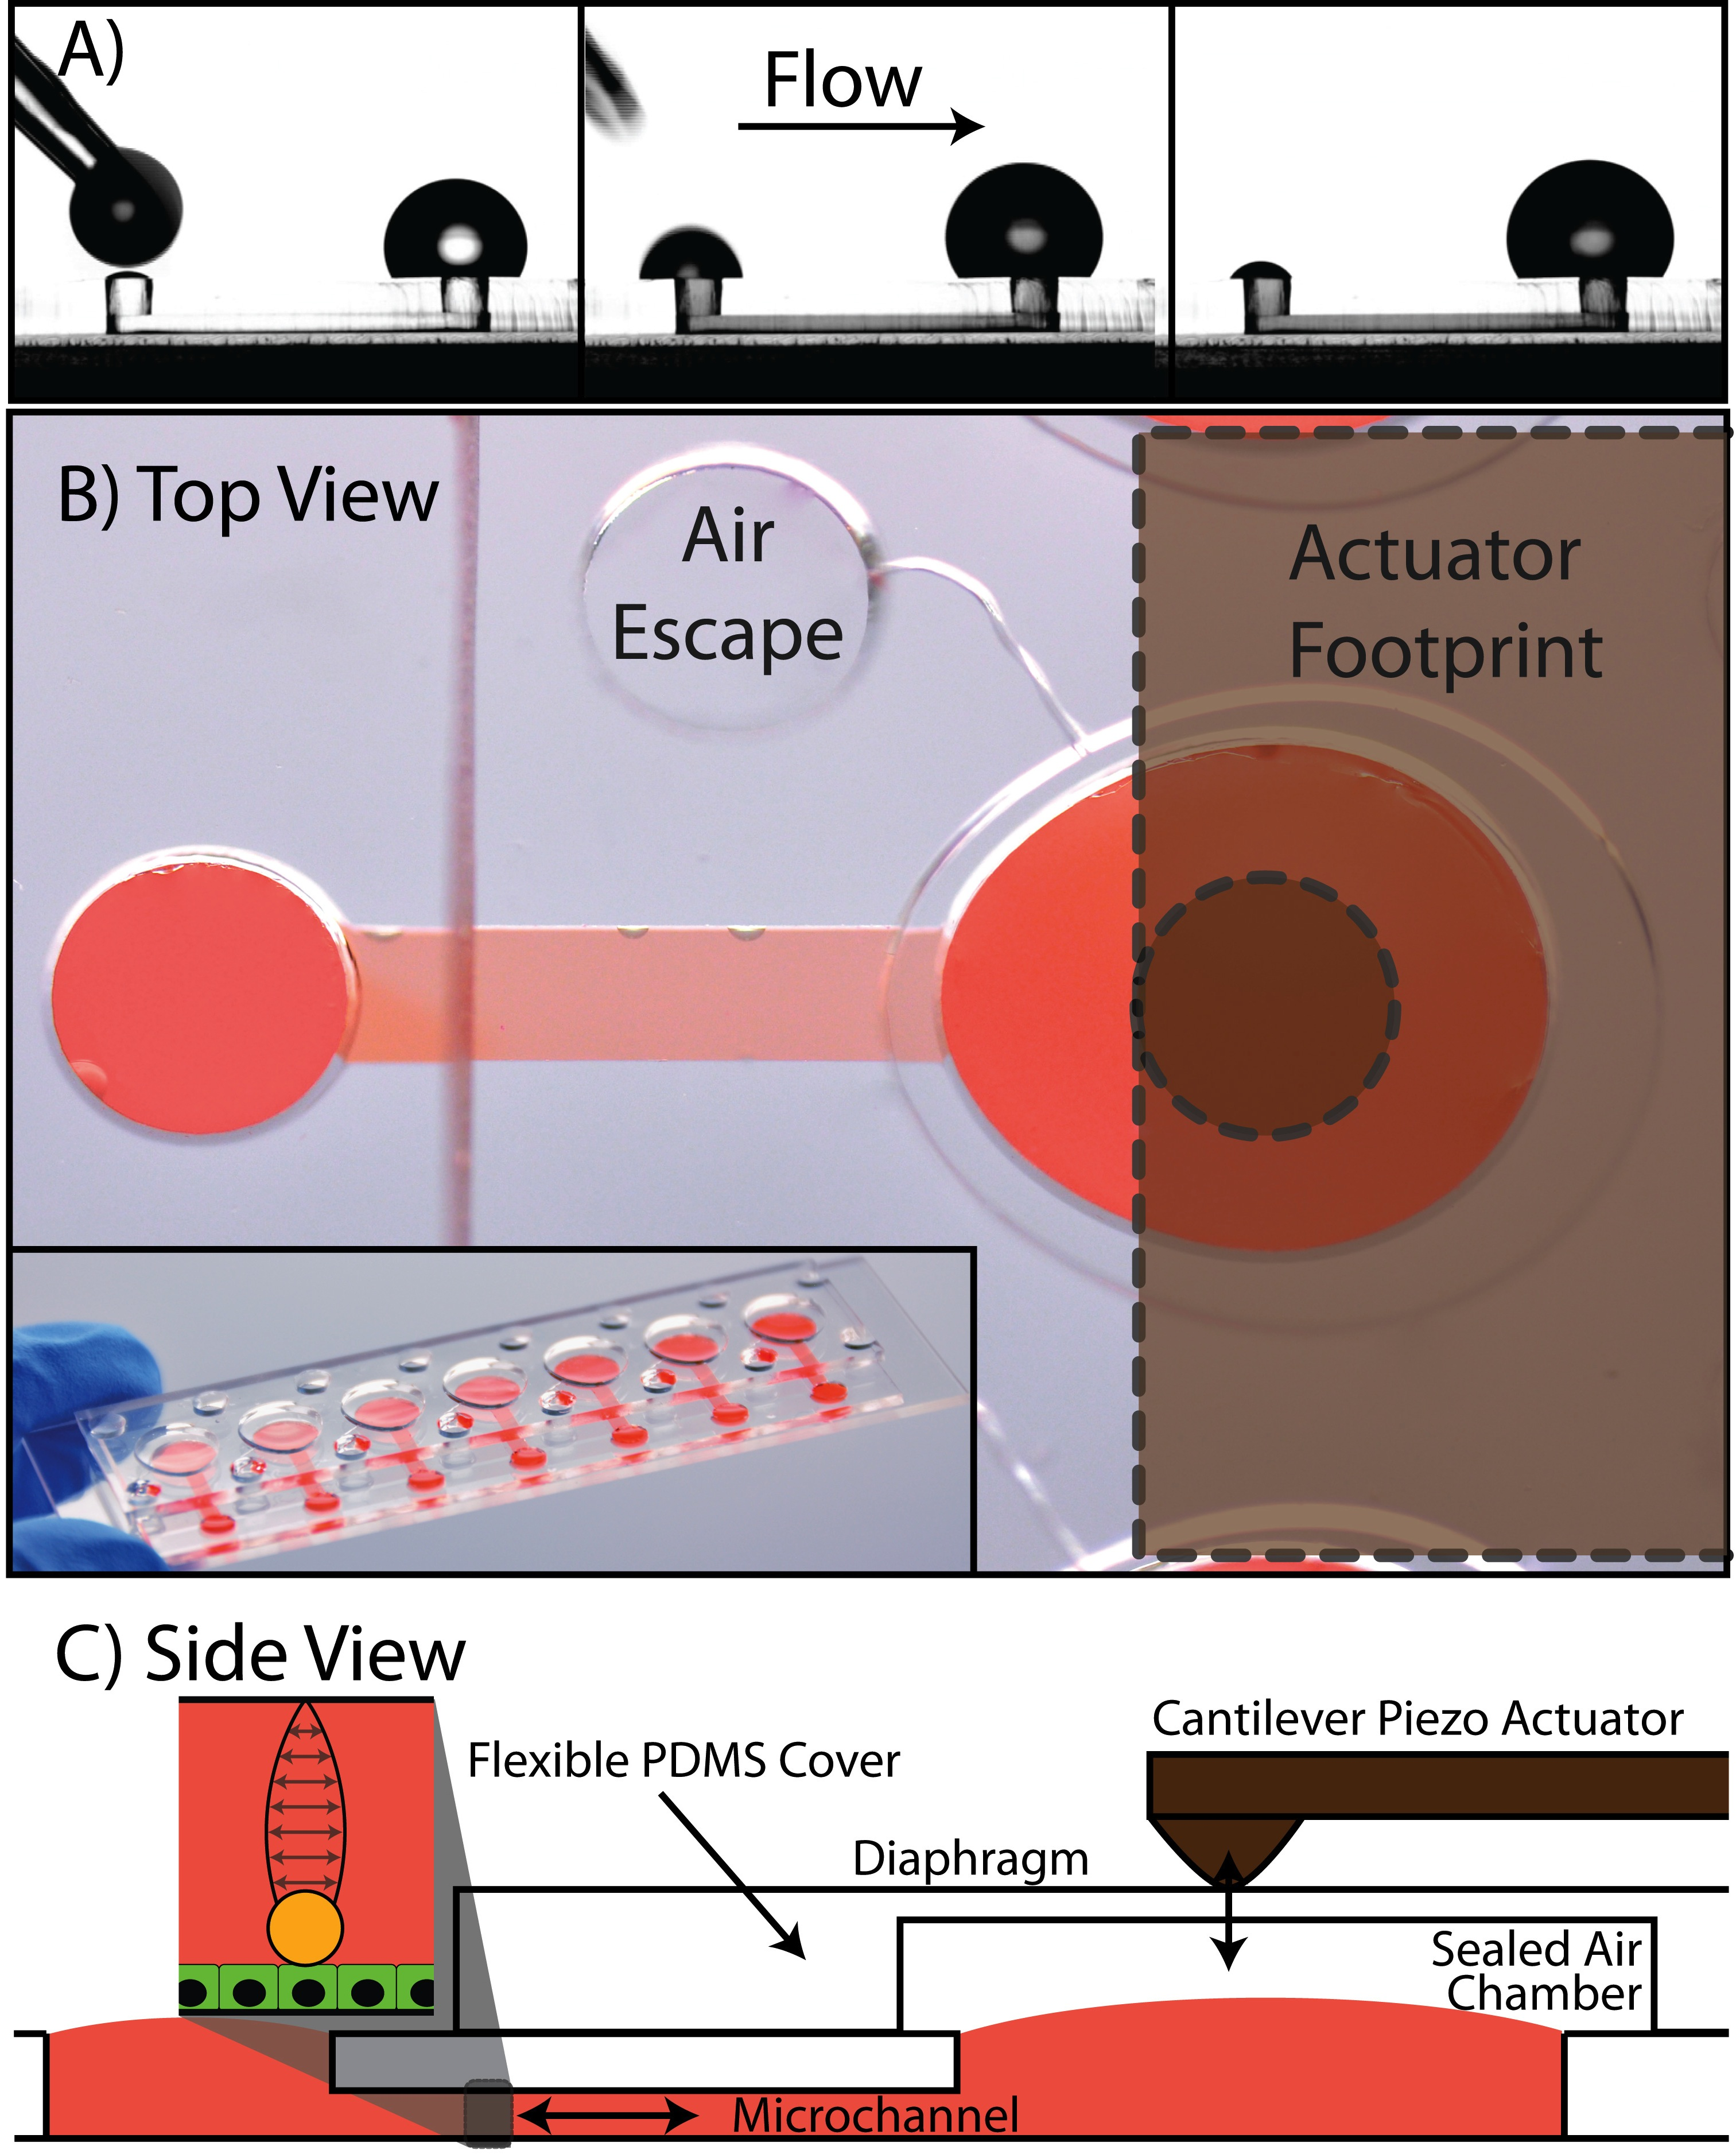
\includegraphics[width=3.5in]{OscillatoryDiagram4.jpg}
\caption{\textbf{Oscillatory flow device}. (A) Side images of passive pumping via dispensed droplets. (B) Top view of microchannel and diaphragm assembly. Inset shows 7 x 1 array of microchannels on a single microscope slide. (C) Side view of setup. Cantilever piezoelectric actuator deflects diaphragm according to applied voltage signals. At low frequency and moderate amplitude, this creates a volume change in the air cavity and displaces fluid in the channel. Oscillatory shear-stresses may be generated with this approach, allowing it to be used for various cell adhesion studies.}
\label{figure:schematic}
\end{figure}

The dimensions of the straight microchannel mimic the dimensions of a conventional parallel-plate flow chamber while the microchannel ports provide the ability to load and treat cells via pipette. The use of microfabrication techniques will allow us to rapidly explore more complex designs in the future. The footprint of the device provides a modest increase in throughput, i.e., up to seven microchannels per array during one microscope acquisition session, but perhaps more importantly, the microchannels were independently addressable. Maintaining separation ensures that each endothelial monolayer is cultured, activated, and\slash or mechanically stimulated as independent biological samples without adverse cross-talk, as is the case in many multiplexed microfluidic systems. In co-culture adhesion studies, this property has the potential for an even larger impact: the system can test limited cell samples, such as those acquired from clinical patients, as demonstrated by our use of $\sim 10^4$ cells per channel. This is a relatively small amount of cells compared to $\sim 10^6$ to $10^7$ cells typically needed for large-scale (mL) continuous flow in parallel-plate flow chambers. We envision that the system can be scaled if necessary to take even fewer cells ($10^2$ or $10^3$ cells), with only minor modifications to microchannel dimensions.

The oscillatory flow methods used here also have potential utility in other biological applications such as cardiovascular and bone mechanobiology, where oscillatory shear-stress has been implicated in important regulatory functions. Macroscale oscillatory flow systems have already been accepted into the laboratory setting while microscale oscillatory systems (and recirculatory systems in general) have also begun to appear \cite{Song:2005p157,Shao:2009p534}; however, the current design is the first oscillatory system to employ passive-pumping, thus combining the advantages of microscale approaches with simple pipette-based operation that obviate the need for tubing that inherently leads to excess dead volume.

The most innovative features of the demonstrated method are the integrated use of the piezoelectric actuator-PDMS membrane, and the development of a unique cell adhesion readout that has potential to offer new biological insights into cell adhesion phenomena. We leveraged the elastic properties of PDMS to create a sealed air chamber and diaphragm with negligible damping effects below 30 Hz and moderate amplitudes. However, oscillatory flow in a microchannel of these dimensions produces non-linear shear-stress response above 5 Hz. Above 5 Hz, the flow profile becomes non-parabolic. Above 30 Hz, the compliance of the air chamber results in significant attenuation of shear-stress. However, a property of laminar flow (steady and pulsatile) is that shear-stress at a given frequency is always linear to the pressure gradient. Clearance between the diaphragm and fluid in the port also limits actuator amplitudes. However, only 30 \textmu m of motion is required to produce the maximum shear-stress used in this study. As mentioned earlier, the microchannel ports act as reservoirs for oscillatory fluid exchange and thus limit the total volume that can be exchanged between the ports per cycle. The adhesion studies to date have been done in the low frequency regime where damping is insignificant leading to a linear relationship between frequency and shear-stress.

\subsection{Adhesion Assay via Image Differencing}

\paragraph{Measurement of Attachment \vs\ Detachment.}The use of a piezoelectric actuator enables the use of a wide variety of signal waveforms and flexible control of the shear-stress protocol. This capability allowed us to develop an 8-minute adhesion assay that samples a large range of frequencies at high resolution using a logarithmic sweep that spans two orders of magnitude (2 Hz to 100 mHz). Thus, this system provides similar resolution to that presented recently by \cite{Christophis:2010fk}. However, in contrast to Christophis \etal\ and other assays that ramp up shear-stress to detect detachment events, we have employed an inverse strategy where cells are initially prevented from adhering by starting at a relatively high shear-stress and then gradually \emph{reducing} shear-stress in order to monitor the \emph{attachment} events instead of \emph{detachment}.

\paragraph{Oscillatory \vs\ Flow-Through Methodologies}Although both oscillatory and flow-through devices can be used to study both attachment and detachment, the use of oscillatory flow fundamentally changes the readout of an attachment assay compared to flow-through devices and provides new insights into adhesion properties that have not been previously obtained. The \emph{attachment} readout of the oscillatory adhesion assay is identical to the \emph{detachment} readout reported by Christophis \etal. In the case of Christophis \etal\, the population of interest is completely defined prior to detachment, enabling them to present detachment results over a range of shear-stresses in terms of ``\% of the entire population of interest''. In doing so, they are able to directly measure the shape of the population distribution with respect to detachment shear-stress. The ability to measure the shape of the population distribution can provide important insight into the mechanisms of adhesion. In our case, the population of interest can also be defined as those cells that are initially in the field-of-view. The oscillatory nature of the flow allows us to monitor this population of interest over time for different levels of shear-stress to report the number of adhered cells as a \% of the entire population at various shear-stresses, thereby directly measuring the shape of the population distribution as well. This is different from other attachment assays that used flow-through or recirculation devices. When flow-through devices (\eg, the Christophis \etal\ device) are used in ``attachment-mode'' it becomes more difficult to define what an entire population is and makes it much more challenging to elucidate the shape of the population distribution. Thus, it is the oscillatory nature of the flow that enables a direct measurement of population distributions for attachment assays.

A previous study by Wang \etal\ used pulsing flow to study cell attachment and leveraged the ability to follow a single cell over time to examine individual attachment events; however, shear-stress in the system is uncharacterized and the readout was not extended to provide information regarding the distribution of the population \cite{Wang:2009kl}. The embodiment also differs significantly from that reported here given the use of tubes and a mechanical pumping mechanism with limited flexibility for defining complex flow patterns. Also, the study used image streams and image differencing to obtain measurements of \emph{cell motion} which were then normalized using knowledge of cell densities and suspension volumes to compare relative amounts of adhesion between two different cell populations at a given shear-stress. Here, a fully automated algorithm uses image difference information to directly measure the percent of cells adhered for an entire population over a range of shear-stresses.

\paragraph{Image Analysis: Preprocessing.}The percent of adhered cells is determined using phase-contrast microscopy. The data set for each channel consists of 41 image streams, each containing 25-170 images depending on the length of time needed to acquire 1-2 cycles of cell motion. The background is subtracted from all the images in the data set. The image used for background subtraction is determined from the first stream of images. In phase contrast using low magnification (2X), the cells appear brighter than the background. Thus, a stack projection is performed on the first stream to determine the minimum intensity for each pixel over time, removing any brighter moving objects (\ie, suspended cells) from the resulting background image. Thus, the background subtracted images in the data set are greatly enhanced to show suspended cells that were added to the channel. By using the same background image to perform all background subtraction for a given channel, any suspeded cells that adhere at a later time-point will still show up as being bright. An Otsu automatic thresholding routine is used to threshold the enhanced images to produce binary images with cells appearing white and background black. The background subtraction process produces stark contrast between the cells and background to make the automatic thresholding routine very robust. A single region of interest (ROI) is then chosen and applied to all images of the data set to restrict analysis from considering portions of the image where no cells exist and where shear-stress is uniform. Given the channel dimensions used in this study, the center 80\% of the channel width exhibits uniform shear-stress and is chosen using the ROI. All subsequent analysis is limited to this ROI.
 
\paragraph{Image Analysis: Quantifying the Percent of Adhered Cells.}Fig \ref{Chap:TumorCellAdhesion:fig:differencing} shows an idealized version of the black and white image streams that result from preprocessing and helps to describe the algorithm used to determine the percent of cells adhered to the substrate. In any given frame of a stream, there can be adhered (A) and non-adhered (NA) cells. In a different frame of the same series, non-adhered cells show up in a different location whereas adhered cells remain in the same spot. Thus, if we take the absolute difference of these two frames the non-adhered cell will show up twice whereas the adhered cell will show up once. Depending on the frames that are chosen, the impressions of the non-adhered cell may partially overlap.

\begin{figure}[!bt]
\centering
\includegraphics[width=6in]{ImageDifferencing.pdf}
\caption{\textbf{Image differencing algorithm}. $F_{n}$ refers to the $n^{th}$ frame of a time-series of images. $F_{n+\Delta n}$ refers an image taken $\Delta n$ frames after $F_{n}$. NA refers to a cell that is \underline{n}ot \underline{a}dhered where as A refers to a cell that is \underline{a}dhered.}
\label{Chap:TumorCellAdhesion:fig:differencing}
\end{figure}

If the impressions do not overlap then Eq \ref{Chap:TumorCellAdhesion:equ:percentAdhered} can be used to predict the percent of cells adhered where $F_{i}$ represents the integrated intensity of the $i^{th}$ binary image. For each stream the reference frame $F_{n}$ is chosen as the frame which exhibits the most average intensity over the course of the stream. The quantity $\left| F_{n}-F_{n+\Delta n}\right|$ is then calculated for all other images while holding $F_{n}$ constant. Partial overlap reduces the value of $\left| F_{n}-F_{n+\Delta n}\right|$ and is expected to occur less than 30\% of the time given our number of frames and minimum cell amplitudes. Therefore the top 5\% of these values are averaged to potentially reduce noise in determining a final value for the numerator of Eq \ref{Chap:TumorCellAdhesion:equ:percentAdhered}. This number is proportional to twice the number of non-adhered cells whereas $F_{n}$ is proportional to the number of total cells, thus arriving at Eq \ref{Chap:TumorCellAdhesion:equ:percentAdhered} for the percent of adhered cells. This process is repeated for each of 41 streams in the data set for each channel to produce a plot of `\% of Population Adhered' \vs\ `Shear-Stress'. It is possible that if oscillation and image acquisition were synchronized, image streams would no longer be necessary as a good choice for $F_{n}$ and $F_{n+\Delta N}$ can be predicted based on the sinusoidal nature of the oscillation.

\begin{equation}
\textrm{\% of Pop. Adhered} = 1 - \frac{\left| F_{n}-F_{n+\Delta n}\right|}{2 \, F_{n}}
\label{Chap:TumorCellAdhesion:equ:percentAdhered}
\end{equation}

\paragraph{Batch Processing.}The image filtering and analysis is completely automated using custom software called Je'Xperiment, developed by Jay Warrick and Erwin Berthier at the University of Wisconsin Madison. The software is used to database the images and perform batch processing of the custom algorithm. One array of 7 channels produces approximately 10-15 gigabytes of data. The primary time constraint of the analysis is thus the time it takes to read and write the images to a hard drive or server ($\sim$ 5 hours total). However, Je'Xperiment allows one to obtain results with less than 10 minutes of time actually invested by the user at the computer workstation.

\paragraph{Interpretation of Results.}Fig \ref{Chap:TumorCellAdhesion:fig:logNorm} illustrates the shape of the resulting adhesion plot and the log-normal cumulative distribution function (LNcdf) used to fit the data. The LNcdf (Eq \ref{Chap:TumorCellAdhesion:equ:LNcdf}) has two parameters, $\mu$ and $\sigma$, which are obtained from the curve fit. The quantity $e^{\mu}$ represents the median shear-stress of the population, $\tau_{50}$, whereas $\sigma$ indicates the spread, measured in orders of magnitude, of the data surrounding the median. This interpretation is different than a normal distribution where $\sigma$ gives an indication of absolute spread about the mean.

\begin{figure}[!t]
\centering
\includegraphics[width=3.5in]{TheoryPlot.pdf}
\caption{\textbf{Log-normal cumulative distribution function}.}
\label{Chap:TumorCellAdhesion:fig:logNorm}
\end{figure}

\begin{equation}
\textrm{LNcdf($x$,$\mu$,$\sigma$)} = \frac{1}{2} + \frac{1}{2}\textrm{erf}\left[ \frac{\ln{x} - \mu}{\sqrt{2 \sigma^{2}}}\right] 
\label{Chap:TumorCellAdhesion:equ:LNcdf}
\end{equation}

Interpretation of changes in the median are fairly straight forward but changes in $\sigma$ are less intuitive. For example, assume there is a cell type and a substrate that interact via one type of molecule with a median shear-stress of 1 Pa and has a $\sigma$ of 1 indicating that 97.89\% of all cells in the population adhere at a shear-stress between 0.1 and 10 Pa. In this idealized scenario, if the substrate is changed such that only 1/10$^{th}$ the original amount of adhesion ligand is presented to the cells, one would expect the median shear-stress to drop to roughly 0.1 Pa given that the number of anchor points per cell is lowered accordingly. Since each portion of the population would fall under this argument, shear-stress data would be predicted to simply shift while keeping $\sigma$ the same. That is to say, the new median shear-stress would be 0.1 Pa with 97.89\% of the population falling between 0.01 and 1 Pa.

On the other hand, what if the median does not change and $\sigma$ does? Given $\sigma$ is a measure of the heterogeneity of the interaction between the cells and substrate, a change in $\sigma$ indicates that the type of mechanism mediating adhesion (\ie\ the involvement of specific molecules or physical forces) has changed or has become more or less heterogeneous. However, it is more likely that multiple molecules or mechanisms mediate adhesion and contribute to an overall perceived heterogeneity. In this situation, if the influence of one of those contributing mechanisms were to be heightened, the value of $\sigma$ would change as well. If a single population has two dominant mechanisms of adhesion, it would result in the multiplication of two characteristic LNcdfs. On the other hand, if there are \emph{two} distinct populations, the result would be the renormalized addition of the two characteristic LNcdfs.

Thus, changes in $\sigma$ are associated with changes in the heterogeneity of the underlying mechanism, whereas changes in the median indicate changes in the strength or number of the interactions.

\subsection{Cancer cell adhesion}
Having defined the oscillatory attachment assay methodology, readout, and method of data interpretation; biological experiments are performed to characterize the sensitivity and repeatability of the assay for detecting physiologically relevant changes in adhesion interactions. We tested adhesion of three established cell lines derived from distinct types of cancer, including prostate (PC3-MM2), breast (MDA-MB231), and multiple myeloma (RPMI8226).  Studies on the adhesiveness, invasiveness and metastatic potential of these cell lines have shown that PC3-MM2 cells are particularly invasive among PC3 family of sublines \cite{Daja:2003rr}, and that PC3 sublines are highly variable in adhesiveness \cite{Dimitroff:2004bh}. MDA-MB231 cells are also highly invasive among breast cancer cell lines \cite{TOZEREN:1995wd,Lee:2003kx}, but are known to adhere to activated endothelium only in the absence of shear-stress $> 0.5$ dyn/cm$^2$ \cite{TOZEREN:1995wd}. In contrast to prostate and breast cancers, the adhesiveness and invasiveness of cells of multiple myeloma (MM) origin has been studied to a much lesser extent. Reports of MM cell adhesion that are available seem to suggest that adhesion to (bone marrow) endothelium is mediated by various molecules other than E-selectin \cite{Okada:1995ys,Broek:2008p301,Katz:2010uq}. Thus, we expected that PC3-MM2 and MDA-MB231 cells would exhibit more adhesive phenotypes, while RPMI8226 would likely show less adhesion to the endothelial monolayers.

We performed independent LNcdf curve fits for each condition, extracted the fitted $\tau_{50}$ and $\sigma$ values and compared results between activated and non-activated endothelium as well as across the different cell types. Fig \ref{Chap:TumorCellAdheison:fig:examples} shows examples of data and LNcdf fits for each cell type on activated and non-activated endothelium.

\begin{figure}[ht] %DONE
\centering
\begin{tabular}{cc}
A) PC3-MM2 & B) RPMI8226 \cr
\includegraphics[width=2.5in]{ExamplePC3.pdf} &\includegraphics[width=2.5in]{ExampleRPMI.pdf} \cr
C) MDA-231 & \cr
\includegraphics[width=2.5in]{ExampleMDA.pdf}
\end{tabular}
\caption{\textbf{Example adhesion curves for each condition}. Each pair of curves represents a adhesion measured in two channels on the same day. (blue) Non-activated endothelium. (red) Activated endothelium. }
\label{Chap:TumorCellAdheison:fig:examples}
\end{figure}

We observed statistically significant increases in $\tau_{50}$ (the critical shear-stress) between activated and non-activated endothelial surfaces for all cell types, including, surprisingly, RPMI8226 cells (Figure \ref{Chap:TumorCellAdhesion:fig:summaryGraphs}A). Comparing non-activated endothelium cases alone, both MDA-MB231 and PC3-MM2 cells exhibited significantly higher values of $\tau_{50}$ than RPMI8226 cells; this was also true for the activated endothelium cases alone, where MDA-MB231 and PC3-MM2 cells had higher $\tau_{50}$ than RPMI8226 cells (Figure \ref{Chap:TumorCellAdhesion:fig:summaryGraphs}A). Interestingly, when the \emph{ratio} between activated and non-activated $\tau_{50}$ values were calculated and compared, no difference was found between cell types (Figure \ref{Chap:TumorCellAdhesion:fig:summaryGraphs}B), suggesting that the effect of IL-1$\beta$ induction on adhesion was consistent across cell types. Thus, MDA-MB231 and PC3-MM2 cells were likely more adhesive than RPMI8226 cells because of intrinsic differences in cell surface properties, which were amplified for all cell types in the presence of E-selectin. This appeared to be consistent with the literature cited above.

\begin{figure}[!tb] %DONE
\centering
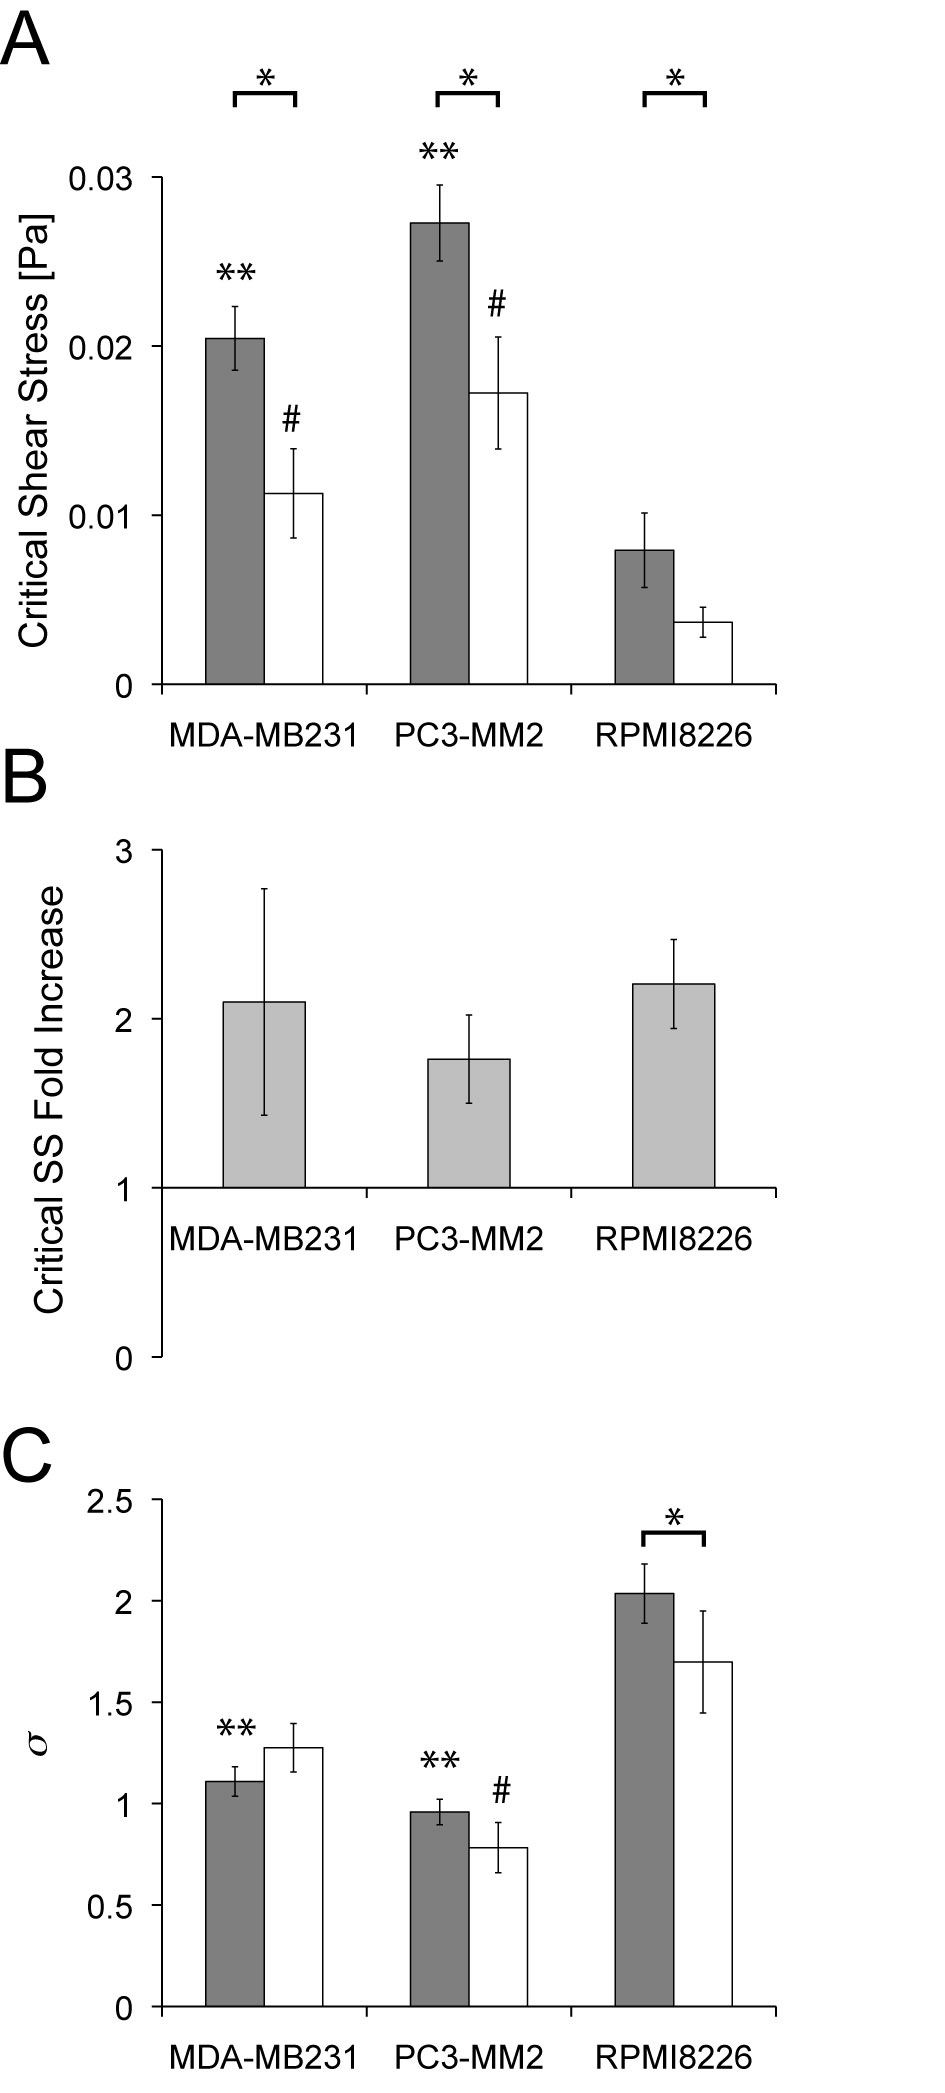
\includegraphics[height=6in]{Figure_FinalGraphs.jpg}
\caption{\textbf{Comparison of adhesion to a HUVEC monolayer}. (A) Average critical shear-stress on activated (gray bars) and non-activated (white bars) endothelium. (B) Average fold increase in critical shear-stress. (C) Average $\sigma$ of lognormal distribution on activated (gray bars) and non-activated (white bars) endothelium. $\ast: P < 0.05$ for combined block multiple experiments between activated and non-activated endothelium for given cell type. $\ast\ast: P < 0.05$ compared to RPMI8226 on activated endothelium.  $\#: P < 0.05$ compared to RPMI8226 non-activated endothelium.}
\label{Chap:TumorCellAdhesion:fig:summaryGraphs}
\end{figure}

Fitted values of $\sigma$ were also compared between non-activated and activated endothelium groups and  across cell types. No statistically significant differences were found between activated and non-activated endothelium conditions for comparisons within each cell type (Figure \ref{Chap:TumorCellAdhesion:fig:summaryGraphs}C). However, $\sigma$ values for RPMI8226 cells were significantly higher than those for PC3-MM2 and MDA-MB231 for both activated and non-activated endothelium groups. These data suggested that $\sigma$, which represents the heterogeneity in cell adhesion of the population, was not influenced by endothelial activation, but only by intrinsic differences between cells. 

Collectively, the pair of fitted parameters $\tau_{50}$ and $\sigma$ have revealed expected yet nevertheless interesting similarities and differences between the cancer cell types, which can be interpreted as follows. No difference in the heterogeneity of the metastatic breast and prostate cancer cell line adhesion could be observed and this heterogeneity did not change significantly upon activation of the endothelium. That is to say, although endothelial activation enhanced adhesion for these two cell types, the level of enhancement was consistent across all individual cells within the population (i.e., no change in spread in the LNcdf was observed), and consistent across cell types (\ie, no significant change in the fold-increase of $\tau_{50}$ was observed either). RPMI8226 cells were similarly affected by endothelial activation, but in comparison to PC3-MM2 and MDA-MB231 cells, RPMI8226 cells were much less adherent and displayed much more heterogeneity in the population. This heterogeneity is potentially related to its low adherence, since loose adhesion from non-specific interactions is likely to yield low $\tau_{50}$ and high $\sigma$. 

\section{Conclusion}
A novel approach for examining cell attachment has been presented that integrates a unique method for producing oscillatory flow, high resolution sweep of shear-stress, fully automated image analysis algorithm, and comprehensive examination of population heterogeneity. The sensitivity and repeatability of the method was validated by confirming an increase in adhesion of three different tumor cell lines representing 3 different cancers to a HUVEC monolayer upon activation of the monolayer using IL-1$\beta$. Unique insight into population heterogeneity was enabled by the use of oscillatory flow. The use of oscillatory flow also enabled the use of passive-pumping to allow samples to be loaded and treated using a pipette. Thus, the platform enables complete separation of microchannels to ensure independence of each data point acquired in the array. Taken together, the method presented here offers new insight into cell adhesion, represents a significant advance to the study of cell attachment, and has the potential to advance our understanding of adhesion in areas such as cancer metastasis, inflammation, and regenerative medicine.

\section{Materials and Methods}

\subsection{Cell Culture}

Human umbilical vein endothelial cells (HUVECs) were purchased from Lonza (Walkersville, MD), and regularly cultured on tissue culture-treated flasks pre-coated with 1.5 $\mu$g/cm$^2$ of bovine plasma fibronectin (FN) (Sigma-Aldrich, St. Louis, MO). HUVECs were maintained in EGM BulletKit media (CC-3124, Lonza) consisting of EBM-2 basal medium supplemented with 2\% fetal bovine serum (FBS), bovine brain extract with heparin, hEGF, hydrocortisone, and gentamicin/Amphotericin B. HUVECs were fed every other day, passaged every 3-4 days at 90\% confluence, and only passages 4-6 were used in microchannel experiments. 

To prepare HUVEC monolayers for adhesion tests, microchannels were first primed with 30 $\mu$L PBS followed by 20 $\mu$L FN at 100 $\mu$g/mL concentration. Microchannels were incubated at 37 deg C for 1 h in humidified trays to allow FN adsorption to the microchannel walls. After incubation, FN was replaced twice with 40 $\mu$L HUVEC media further supplemented with 10 mM HEPES. HUVECs were seeded at 3000 cells/$\mu$L $\times$ 6 $\mu$L per microchannel, and allowed to adhere and culture overnight (12 h). HUVEC microscale cultures were either used on the same day for adhesion tests if confluent, or maintained for an additional day to reach full confluence. Activated HUVEC monolayers in microchannels were induced with 10 $\mu$g/mL interleukin-1$\beta$ (IL-1$\beta$) for 4 h before adhesion tests.

Three different human cancer cell lines were used in adhesion tests to compare adhesion strengths on activated versus non-activated endothelium. MDA-MB231 cells (mammary gland epithelial) were maintained in DMEM with 4.5 g/L glucose supplemented with 10\% FBS and 1\% penicillin/streptomycin (P/S). PC-3 MM2 cells (metastatic prostate) were maintained in RPMI1640 with L-glutamine, 10\% FBS, 1\% penicillin/streptomycin (P/S), and 10 mM HEPES. RPMI8226 cells (multiple myeloma in bone marrow) were maintained in DMEM with 4.5 g/L glucose supplemented with 10\% FBS, 1\% P/S, and 10 mM HEPES.  MDA-MB231 and PC3-MM2 cells were fed every other day and passaged every 3-4 days depending on confluence. RPMI8226 cells were passaged every 3 days. All cell lines were resuspended at 1000-1500 cells/$\mu$L, and 7.5 $\mu$L of cell suspension was dispensed into each microchannel. Thus, each microchannel contained approx. 7,500 to 12,000 cells.

\subsection{Immunostaining and HUVEC activation}

Immunostaining was performed to verify upregulation of E-selectin upon activation using IL-1$\beta$. Fig \ref{Chap:TumorCellAdhesion:fig:staining} shows that E-selectin upregulation was robust for all concentrations tested while the control showed basal levels. Acquisition parameters were identical and images were treated uniformly.

\begin{figure}[!ht]
\centering
\includegraphics[width=3.5in]{StainingImages.pdf}
\caption{\textbf{HUVEC staining for E-selectin}. Concentration of IL-1$\beta$ is indicated in the corner of each image.}
\label{Chap:TumorCellAdhesion:fig:staining}
\end{figure}


\subsection{Image Capture and Analysis}

Prior to data acquisition, a calibration procedure described in Chapter \ref{Chap:Oscillator} was used to measure the initial shear stress of the system at 140 mV piezo voltage and 2 Hz sinusoidal oscillation frequency. The actuator was perturbed by gentle tapping to redistribute cells within the field of view that moved due to the calibration procedure. After waiting 30 seconds for cells to settle, the acquisition protocol was started.

Data acquisition consists of 41 stream acquisitions. The first 5 are to be acquired at 2 Hz. At the start of the sixth stream, a descending log frequency sweep is begun that lasts for 500 s and ends at 0.1 Hz. The first six datapoints obtained at a frequency of 2 Hz are used to normalize each curve. The average of those six measurements is forced to a value of one resulting in a proportional adjustment of all other values.

MetaMorph was used to acquire the image streams at specified intervals of time using the journaling capability of the software. The software also allows for the logging of times. The time at the beginning of each image stream is recorded to allow back-calculation of the frequency. This is helps improve accuracy because MetaMorph is not able to perform each stream acquisition at precisely the same time for each channel due to variability in data read-write times. The number of frames per stream was chosen to ensure capture of 1-2 cycles of fluid\slash cell motion and ranged from 25 to 170. Variable numbers of frames were used to limit the amount of data.

Images were acquired at 2X with a binning of 2 $\times$ 2 and an exposure time of 15 ms. The Ph1/PhC phase rings were used to provide maximal contrast (\ie, dark background and bright cells).

\subsection{Statistical Analyses}

\paragraph{Effects of activation.} Median $\tau_{50}$ and standard deviation $\sigma$ were determined from the lognormal curve fits for each condition (HUVEC activation and cell type), and statistically compared using nonparametric tests. First, to determine whether activation of HUVEC monolayers via IL-1beta induction had an effect on cell adhesion for each cell type, we used a combined Wilcoxon rank sum approach proposed by Lehmann (1998) for handling the complete data set consisting of multiple experiments with varying sample sizes. This required that we group our data into blocks for the separate experiments, with each block consisting of $m$ activated and $n$ non-activated monolayers.

\paragraph{Differences between cell type.} Independent Kruskal-Wallis tests were used to determine whether differences in $\tau_{50}$ and $\sigma$ were present across cell types for both the activated and non-activated monolayers. We further normalized $tau_{50}$ by defining the ratio or ``fold-increase'' of activated to non-activated adhesion, and performed Kruskal-Wallis analysis on normalized $tau_{50}$. All Kruskal-Wallis tests were performed on values averaged across samples in the same experiment.

When Kruskal-Wallis tests revealed significant differences in the data, post hoc multiple comparison tests were performed via independent Wilcoxon rank-sum tests, with and without Bonferroni correction, between separate pairs of cell types to determine which cell types differed from the others. 

\paragraph{Outliers.} Coefficients of determination ($R^{2}$) were calculated for each curve fit, and it was found that $R^{2}$ = 0.94 +/- 0.06 for the fifty experiments we conducted. One outlier was detected ($R^{2}$ = 0.60), and removal of the outlier resulted in $R^{2}$ = 0.95 +/- 0.04. The above statistical tests were done with both inclusion and exclusion of the outlier, and it was found that the main conclusions were not affected by the presence of the outlier.





\chapter{Assays: Cell Adhesion Assay Validation: Tumor-Cell Adhesion to a HUVEC Monolayer}
\label{Chap:TumorCellAdhesion}

\section{Preface}
This work was performed and written in equal collaboration with Edmond Young as represents a manuscript in preparation.

\section{Introduction}
The process of cell adhesion involves physical interactions between cells and the materials in their microenvironment such as extracellular matrices, synthetic biomaterial surfaces, and other cells and is a major topic of interest in areas ranging from fundamental cell biology and pathophysiology \cite{Chen:1997p320,Davies:1995p87} to tissue engineering and regeneration \cite{Nugent:2003p459}. In particular, cell adhesion plays an integral role in inflammation and cancer metastasis where leukocytes and circulating neoplastic cells, respectively, interact with the vascular endothelium in complex adhesion cascades that include tethering, rolling, spreading and endothelial transmigration events \cite{Ley:2007fk,Geiger:2009vn}. The ability to examine and measure the propensity of cells to adhere to the endothelium or other surfaces (engineered or natural) and determine the strength of adhesion is thus critically important to advancing our understanding of the mechanisms related to inflammation and cancer and to the development of tissue engineering strategies in regenerative medicine.

While cell adhesion fundamentally relies on the biophysical and biochemical properties of individual cells \cite{Orsello:2001uq}, many adhesion studies use population-based assays to determine global adhesion characteristics that efficiently reveal important and relevant properties of the cell population \cite{Christ:2010ly}. Population-based adhesion assays typically depend on fluid-flow systems that generate mechanical shear-stress, providing means to promote or challenge adhesion to the substrate on interest in a controlled manner. The most common fluid-flow systems for studying cell adhesion include the parallel-plate flow chamber \cite{GIAVAZZI:1993ty}, radial flow chamber \cite{Goldstein:2002p106}, cone-and-plate viscometer \cite{Jadhav:2001ys}, variable width devices \cite{Heilshorn:2003ly,Usami:1993p603}, and variable-height chambers \cite{Xiao:1996p618}. These systems typically employ steady flow conditions, but they can also be readily modified to accommodate oscillatory or pulsatile flow conditions for studies in shear-mediated atherosclerosis and cardiovascular pathobiology \cite{KU:1985uq,Chappell:1998fk}. Depending on the purpose of the study and availability of resources, flow systems can be operated under various schemes or protocols to produce different types of adhesion assays. For example, flow-rate\slash shear-stress can either be increased or decreased in a stepwise fashion to assay the gradual detachment or attachment of cells, respectively. Furthermore, shear-stress ranges can be expanded, or the number of steps in the ramping scheme can be increased to yield a more continuous scheme with better resolution for detecting adhesion events than more discrete protocols. Although fluid-flow systems have become indispensable tools in biological research, these systems have significant drawbacks due to their large scale, complex setup, and need for large volumes of medium and cell suspension to maintain flow. 

Recently, a number of microfluidic systems have been developed for cell adhesion and shear-flow assays \cite{Lu:2004ys,Gutierrez:2007p290,Plouffe:2007p274,Young:2007ml}, taking advantage of microfabrication techniques to create systems that can increase throughput, handle reduced fluid volumes, and improve spatiotemporal control of \invitro\ microenvironments \cite{Young:2010p286,Young:2010uq}. While these microscale flow systems have shown improvements over their macroscale counterparts and have overcome some of the main drawbacks of previous systems, the majority of microfluidic systems continue to require complex ``world-to-chip'' interfacing \cite{Fredrickson:2004ve} that limits their potential for widespread adoption in biology labs, particularly in clinical and translational research applications where limited patient-derived cell and tissue samples may be significantly depleted by excessive tubing and large dead volumes. 

We have developed a novel microscale system for conducting oscillatory, shear adhesion assays that employs passive-pumping principles to eliminate cumbersome interconnects and unnecessary tubes and dead volume. The system, described in detail below, enables pipette-based loading and treatments, is easily amenable to complex microscale geometries, and can be dynamically controlled to offer various oscillatory waveforms for cardiovascular applications. Most importantly, this microscale system offers analysis of the adherence of a small and defined population of cells in a manner that cannot be achieved with existing systems, thus enabling studies of limited cell samples such as those acquired from a clinical setting. These capabilities, coupled with a custom information-rich readout, allow this system to be applied to a wide range of biological experiments. To illustrate the potential of this system and custom readout, we developed an attachment-based adhesion assay that utilizes a decreasing log-sweep of shear-stress and differential image analysis of image-streams to quantify the process of adhesion for an entire population of interest. We used the integrated system to study adhesion of three different cancer cell-lines on activated and non-activated endothelial monolayers. Results demonstrate the ability of this approach to provide new insights into the heterogeneity of cell populations and adhesion mechanisms.

\section{Results and Discussion}

\subsection{System Design and Operation}

Our main objective was to design, test, and implement a passive-pumping-based oscillatory flow system for an array of microchannels in order to extend oscillatory modes of shear flow to pipette friendly systems.  Passive-pumping has been used previously in various applications, and has been described in detail elsewhere \cite{Berthier:2007mi,Meyvantsson:2008,Walker:2004ov}. Briefly, passive-pumping leverages surface tension to pump fluid from small droplets to larger droplets based on Laplace's law (Figure \ref{figure:schematic}A). We fabricated a simple one-input-one-output straight microchannel where one port is smaller than the other to facilitate passive-pumping of cell suspensions, media, and reagents. To generate oscillatory flow, we further designed and fabricated a diaphragm from polydimethylsiloxane (PDMS) that was positioned over the larger outlet port and reversibly sealed to the top of the PDMS microchannel. The diaphragm was actuated using a piezoelectric cantilever which bends in response to a voltage signal. The actuator was retrofitted with an adjustable cap screw to provide a single point of contact between the actuator and diaphragm (Figure \ref{figure:schematic}B). Voltage signals were produced using a function generator and passed through an amplifier to the actuator to tunably control displacement of the cap screw tip. The resulting deflections of the diaphragm induce pressure changes within the sealed air chamber below the diaphragm to drive oscillatory flow within the microchannel. The ports act as reservoirs for volume fluctuations with the exposed port providing pipette access to deliver treatments or cell suspension.

\begin{figure}[ht] %DONE
\centering
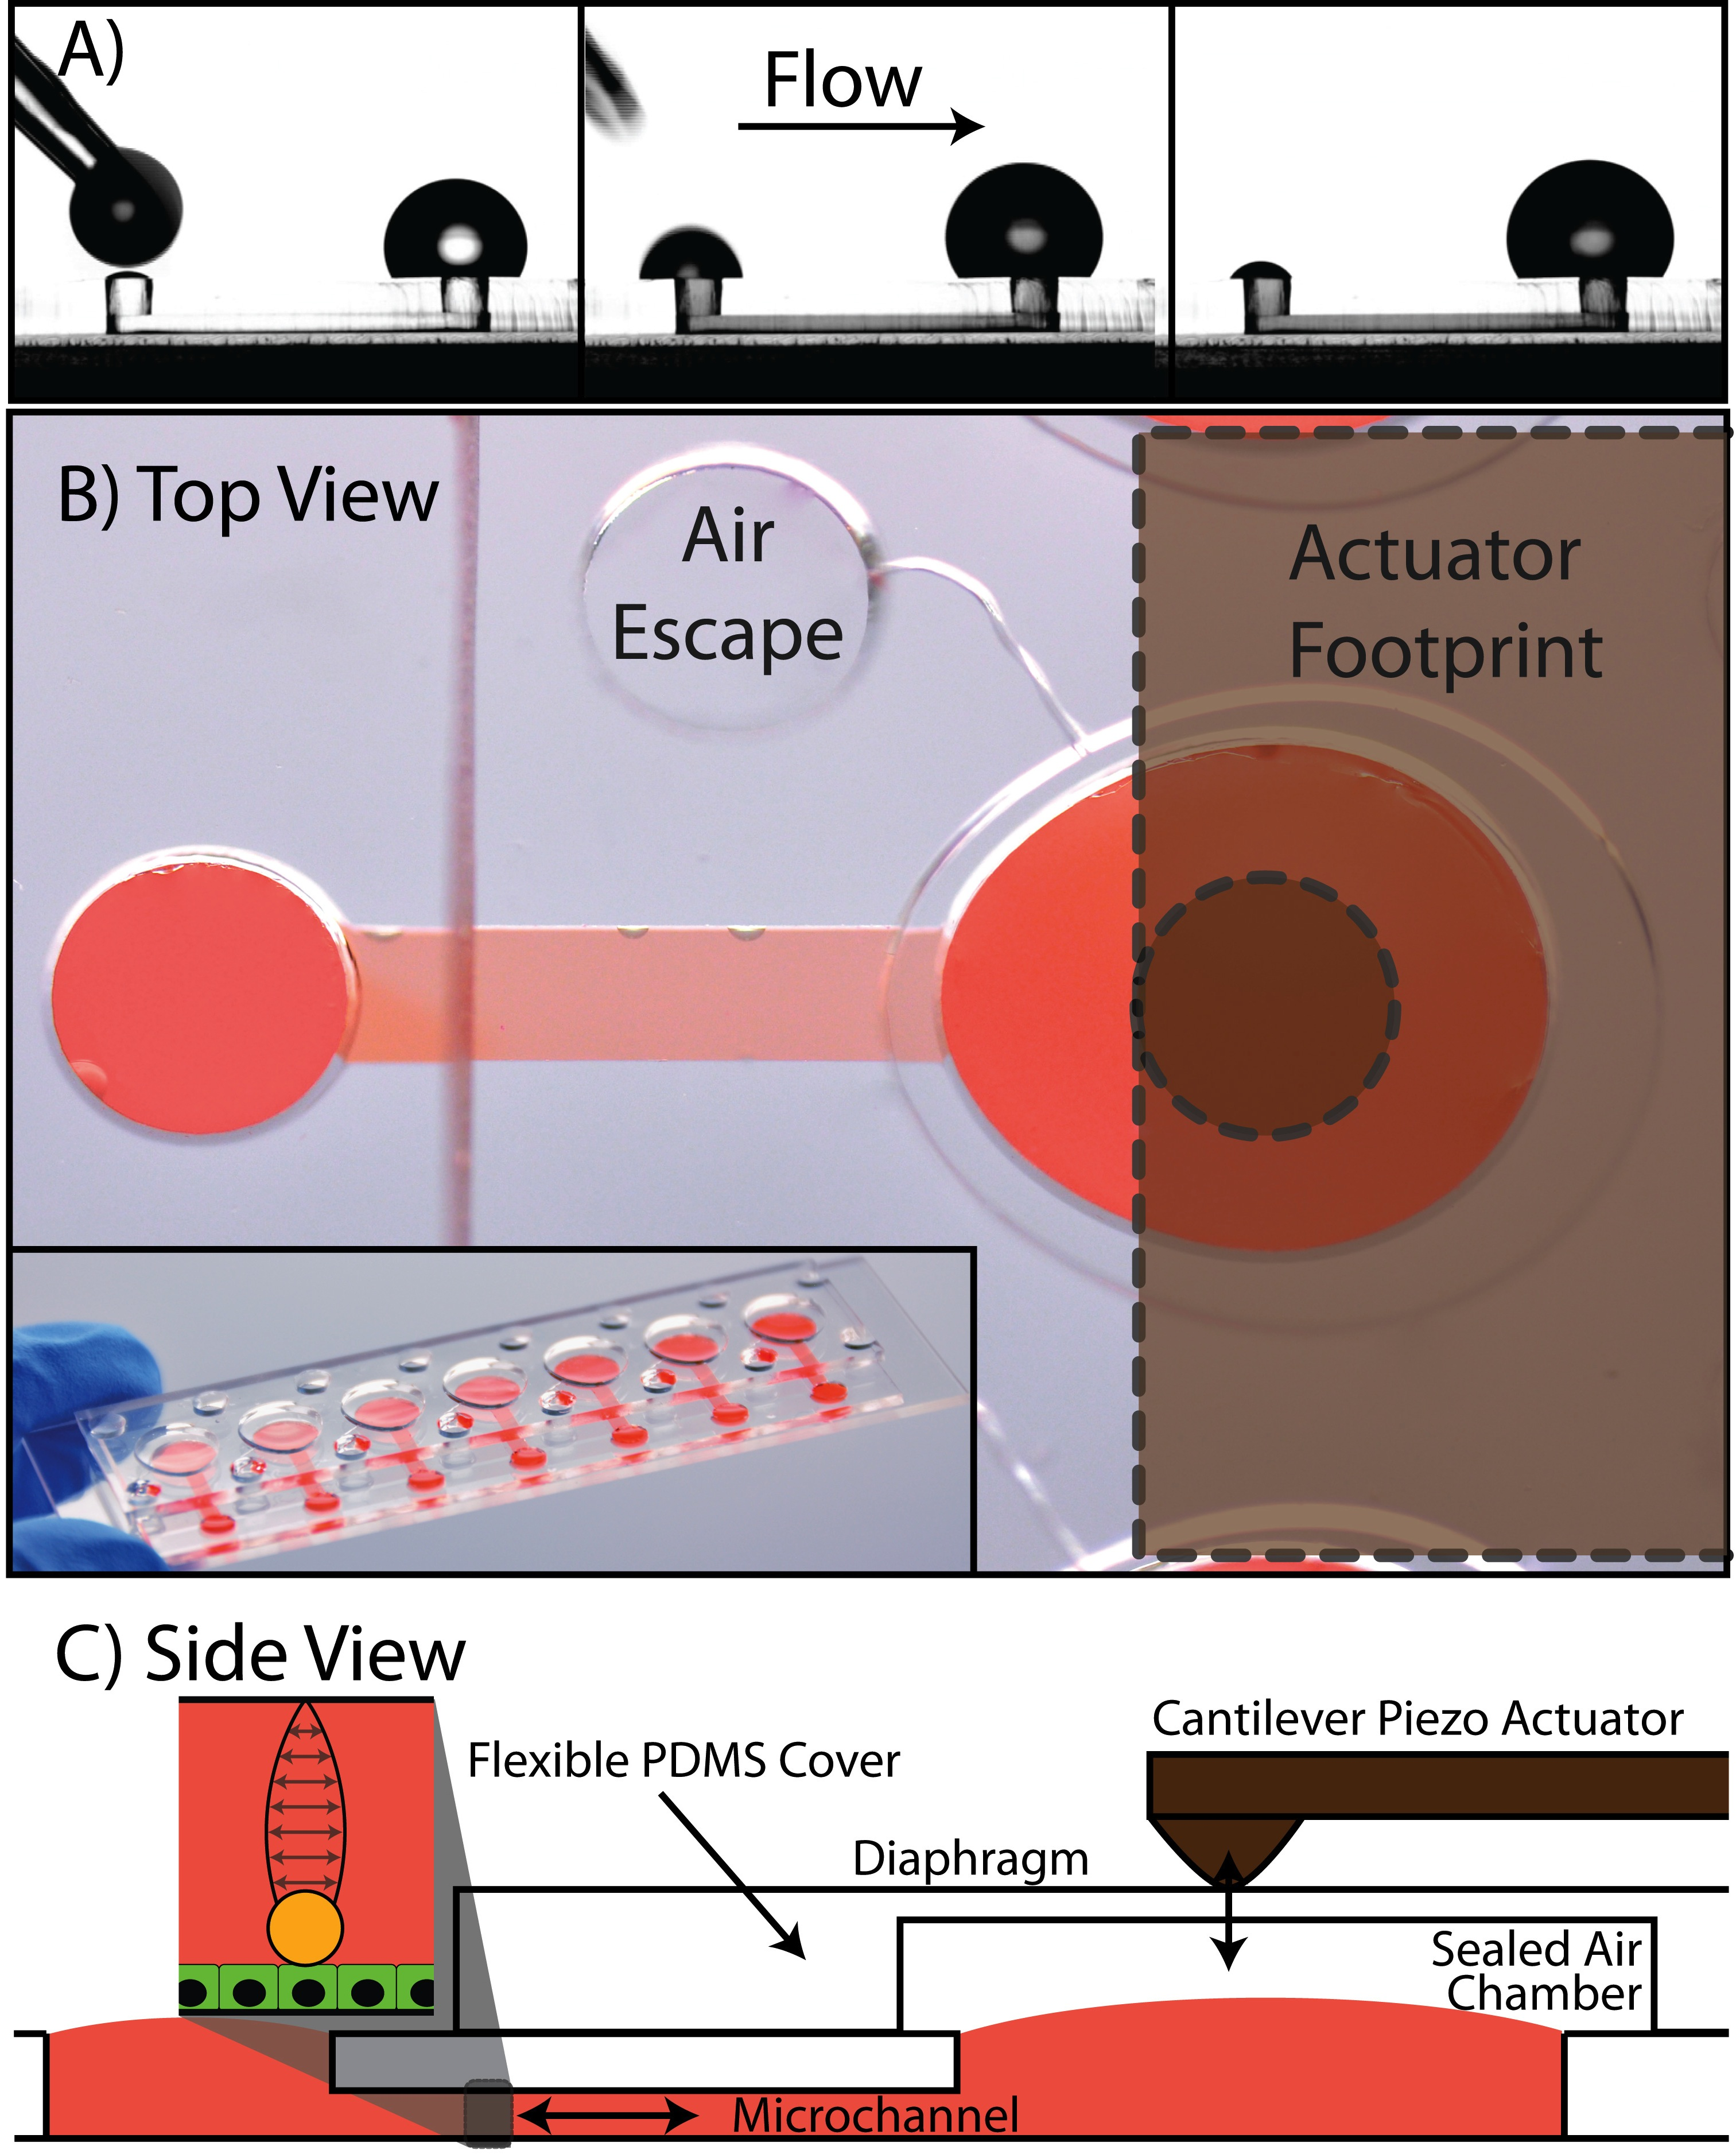
\includegraphics[width=3.5in]{OscillatoryDiagram4.jpg}
\caption{\textbf{Oscillatory flow device}. (A) Side images of passive pumping via dispensed droplets. (B) Top view of microchannel and diaphragm assembly. Inset shows 7 x 1 array of microchannels on a single microscope slide. (C) Side view of setup. Cantilever piezoelectric actuator deflects diaphragm according to applied voltage signals. At low frequency and moderate amplitude, this creates a volume change in the air cavity and displaces fluid in the channel. Oscillatory shear-stresses may be generated with this approach, allowing it to be used for various cell adhesion studies.}
\label{figure:schematic}
\end{figure}

The dimensions of the straight microchannel mimic the dimensions of a conventional parallel-plate flow chamber while the microchannel ports provide the ability to load and treat cells via pipette. The use of microfabrication techniques will allow us to rapidly explore more complex designs in the future. The footprint of the device provides a modest increase in throughput, i.e., up to seven microchannels per array during one microscope acquisition session, but perhaps more importantly, the microchannels were independently addressable. Maintaining separation ensures that each endothelial monolayer is cultured, activated, and\slash or mechanically stimulated as independent biological samples without adverse cross-talk, as is the case in many multiplexed microfluidic systems. In co-culture adhesion studies, this property has the potential for an even larger impact: the system can test limited cell samples, such as those acquired from clinical patients, as demonstrated by our use of $\sim 10^4$ cells per channel. This is a relatively small amount of cells compared to $\sim 10^6$ to $10^7$ cells typically needed for large-scale (mL) continuous flow in parallel-plate flow chambers. We envision that the system can be scaled if necessary to take even fewer cells ($10^2$ or $10^3$ cells), with only minor modifications to microchannel dimensions.

The oscillatory flow methods used here also have potential utility in other biological applications such as cardiovascular and bone mechanobiology, where oscillatory shear-stress has been implicated in important regulatory functions. Macroscale oscillatory flow systems have already been accepted into the laboratory setting while microscale oscillatory systems (and recirculatory systems in general) have also begun to appear \cite{Song:2005p157,Shao:2009p534}; however, the current design is the first oscillatory system to employ passive-pumping, thus combining the advantages of microscale approaches with simple pipette-based operation that obviate the need for tubing that inherently leads to excess dead volume.

The most innovative features of the demonstrated method are the integrated use of the piezoelectric actuator-PDMS membrane, and the development of a unique cell adhesion readout that has potential to offer new biological insights into cell adhesion phenomena. We leveraged the elastic properties of PDMS to create a sealed air chamber and diaphragm with negligible damping effects below 30 Hz and moderate amplitudes. However, oscillatory flow in a microchannel of these dimensions produces non-linear shear-stress response above 5 Hz. Above 5 Hz, the flow profile becomes non-parabolic. Above 30 Hz, the compliance of the air chamber results in significant attenuation of shear-stress. However, a property of laminar flow (steady and pulsatile) is that shear-stress at a given frequency is always linear to the pressure gradient. Clearance between the diaphragm and fluid in the port also limits actuator amplitudes. However, only 30 \textmu m of motion is required to produce the maximum shear-stress used in this study. As mentioned earlier, the microchannel ports act as reservoirs for oscillatory fluid exchange and thus limit the total volume that can be exchanged between the ports per cycle. The adhesion studies to date have been done in the low frequency regime where damping is insignificant leading to a linear relationship between frequency and shear-stress.

\subsection{Adhesion Assay via Image Differencing}

\paragraph{Measurement of Attachment \vs\ Detachment.}The use of a piezoelectric actuator enables the use of a wide variety of signal waveforms and flexible control of the shear-stress protocol. This capability allowed us to develop an 8-minute adhesion assay that samples a large range of frequencies at high resolution using a logarithmic sweep that spans two orders of magnitude (2 Hz to 100 mHz). Thus, this system provides similar resolution to that presented recently by \cite{Christophis:2010fk}. However, in contrast to Christophis \etal\ and other assays that ramp up shear-stress to detect detachment events, we have employed an inverse strategy where cells are initially prevented from adhering by starting at a relatively high shear-stress and then gradually \emph{reducing} shear-stress in order to monitor the \emph{attachment} events instead of \emph{detachment}.

\paragraph{Oscillatory \vs\ Flow-Through Methodologies}Although both oscillatory and flow-through devices can be used to study both attachment and detachment, the use of oscillatory flow fundamentally changes the readout of an attachment assay compared to flow-through devices and provides new insights into adhesion properties that have not been previously obtained. The \emph{attachment} readout of the oscillatory adhesion assay is identical to the \emph{detachment} readout reported by Christophis \etal. In the case of Christophis \etal\, the population of interest is completely defined prior to detachment, enabling them to present detachment results over a range of shear-stresses in terms of ``\% of the entire population of interest''. In doing so, they are able to directly measure the shape of the population distribution with respect to detachment shear-stress. The ability to measure the shape of the population distribution can provide important insight into the mechanisms of adhesion. In our case, the population of interest can also be defined as those cells that are initially in the field-of-view. The oscillatory nature of the flow allows us to monitor this population of interest over time for different levels of shear-stress to report the number of adhered cells as a \% of the entire population at various shear-stresses, thereby directly measuring the shape of the population distribution as well. This is different from other attachment assays that used flow-through or recirculation devices. When flow-through devices (\eg, the Christophis \etal\ device) are used in ``attachment-mode'' it becomes more difficult to define what an entire population is and makes it much more challenging to elucidate the shape of the population distribution. Thus, it is the oscillatory nature of the flow that enables a direct measurement of population distributions for attachment assays.

A previous study by Wang \etal\ used pulsing flow to study cell attachment and leveraged the ability to follow a single cell over time to examine individual attachment events; however, shear-stress in the system is uncharacterized and the readout was not extended to provide information regarding the distribution of the population \cite{Wang:2009kl}. The embodiment also differs significantly from that reported here given the use of tubes and a mechanical pumping mechanism with limited flexibility for defining complex flow patterns. Also, the study used image streams and image differencing to obtain measurements of \emph{cell motion} which were then normalized using knowledge of cell densities and suspension volumes to compare relative amounts of adhesion between two different cell populations at a given shear-stress. Here, a fully automated algorithm uses image difference information to directly measure the percent of cells adhered for an entire population over a range of shear-stresses.

\paragraph{Image Analysis: Preprocessing.}The percent of adhered cells is determined using phase-contrast microscopy. The data set for each channel consists of 41 image streams, each containing 25-170 images depending on the length of time needed to acquire 1-2 cycles of cell motion. The background is subtracted from all the images in the data set. The image used for background subtraction is determined from the first stream of images. In phase contrast using low magnification (2X), the cells appear brighter than the background. Thus, a stack projection is performed on the first stream to determine the minimum intensity for each pixel over time, removing any brighter moving objects (\ie, suspended cells) from the resulting background image. Thus, the background subtracted images in the data set are greatly enhanced to show suspended cells that were added to the channel. By using the same background image to perform all background subtraction for a given channel, any suspeded cells that adhere at a later time-point will still show up as being bright. An Otsu automatic thresholding routine is used to threshold the enhanced images to produce binary images with cells appearing white and background black. The background subtraction process produces stark contrast between the cells and background to make the automatic thresholding routine very robust. A single region of interest (ROI) is then chosen and applied to all images of the data set to restrict analysis from considering portions of the image where no cells exist and where shear-stress is uniform. Given the channel dimensions used in this study, the center 80\% of the channel width exhibits uniform shear-stress and is chosen using the ROI. All subsequent analysis is limited to this ROI.
 
\paragraph{Image Analysis: Quantifying the Percent of Adhered Cells.}Fig \ref{Chap:TumorCellAdhesion:fig:differencing} shows an idealized version of the black and white image streams that result from preprocessing and helps to describe the algorithm used to determine the percent of cells adhered to the substrate. In any given frame of a stream, there can be adhered (A) and non-adhered (NA) cells. In a different frame of the same series, non-adhered cells show up in a different location whereas adhered cells remain in the same spot. Thus, if we take the absolute difference of these two frames the non-adhered cell will show up twice whereas the adhered cell will show up once. Depending on the frames that are chosen, the impressions of the non-adhered cell may partially overlap.

\begin{figure}[!bt]
\centering
\includegraphics[width=6in]{ImageDifferencing.pdf}
\caption{\textbf{Image differencing algorithm}. $F_{n}$ refers to the $n^{th}$ frame of a time-series of images. $F_{n+\Delta n}$ refers an image taken $\Delta n$ frames after $F_{n}$. NA refers to a cell that is \underline{n}ot \underline{a}dhered where as A refers to a cell that is \underline{a}dhered.}
\label{Chap:TumorCellAdhesion:fig:differencing}
\end{figure}

If the impressions do not overlap then Eq \ref{Chap:TumorCellAdhesion:equ:percentAdhered} can be used to predict the percent of cells adhered where $F_{i}$ represents the integrated intensity of the $i^{th}$ binary image. For each stream the reference frame $F_{n}$ is chosen as the frame which exhibits the most average intensity over the course of the stream. The quantity $\left| F_{n}-F_{n+\Delta n}\right|$ is then calculated for all other images while holding $F_{n}$ constant. Partial overlap reduces the value of $\left| F_{n}-F_{n+\Delta n}\right|$ and is expected to occur less than 30\% of the time given our number of frames and minimum cell amplitudes. Therefore the top 5\% of these values are averaged to potentially reduce noise in determining a final value for the numerator of Eq \ref{Chap:TumorCellAdhesion:equ:percentAdhered}. This number is proportional to twice the number of non-adhered cells whereas $F_{n}$ is proportional to the number of total cells, thus arriving at Eq \ref{Chap:TumorCellAdhesion:equ:percentAdhered} for the percent of adhered cells. This process is repeated for each of 41 streams in the data set for each channel to produce a plot of `\% of Population Adhered' \vs\ `Shear-Stress'. It is possible that if oscillation and image acquisition were synchronized, image streams would no longer be necessary as a good choice for $F_{n}$ and $F_{n+\Delta N}$ can be predicted based on the sinusoidal nature of the oscillation.

\begin{equation}
\textrm{\% of Pop. Adhered} = 1 - \frac{\left| F_{n}-F_{n+\Delta n}\right|}{2 \, F_{n}}
\label{Chap:TumorCellAdhesion:equ:percentAdhered}
\end{equation}

\paragraph{Batch Processing.}The image filtering and analysis is completely automated using custom software called Je'Xperiment, developed by Jay Warrick and Erwin Berthier at the University of Wisconsin Madison. The software is used to database the images and perform batch processing of the custom algorithm. One array of 7 channels produces approximately 10-15 gigabytes of data. The primary time constraint of the analysis is thus the time it takes to read and write the images to a hard drive or server ($\sim$ 5 hours total). However, Je'Xperiment allows one to obtain results with less than 10 minutes of time actually invested by the user at the computer workstation.

\paragraph{Interpretation of Results.}Fig \ref{Chap:TumorCellAdhesion:fig:logNorm} illustrates the shape of the resulting adhesion plot and the log-normal cumulative distribution function (LNcdf) used to fit the data. The LNcdf (Eq \ref{Chap:TumorCellAdhesion:equ:LNcdf}) has two parameters, $\mu$ and $\sigma$, which are obtained from the curve fit. The quantity $e^{\mu}$ represents the median shear-stress of the population, $\tau_{50}$, whereas $\sigma$ indicates the spread, measured in orders of magnitude, of the data surrounding the median. This interpretation is different than a normal distribution where $\sigma$ gives an indication of absolute spread about the mean.

\begin{figure}[!t]
\centering
\includegraphics[width=3.5in]{TheoryPlot.pdf}
\caption{\textbf{Log-normal cumulative distribution function}.}
\label{Chap:TumorCellAdhesion:fig:logNorm}
\end{figure}

\begin{equation}
\textrm{LNcdf($x$,$\mu$,$\sigma$)} = \frac{1}{2} + \frac{1}{2}\textrm{erf}\left[ \frac{\ln{x} - \mu}{\sqrt{2 \sigma^{2}}}\right] 
\label{Chap:TumorCellAdhesion:equ:LNcdf}
\end{equation}

Interpretation of changes in the median are fairly straight forward but changes in $\sigma$ are less intuitive. For example, assume there is a cell type and a substrate that interact via one type of molecule with a median shear-stress of 1 Pa and has a $\sigma$ of 1 indicating that 97.89\% of all cells in the population adhere at a shear-stress between 0.1 and 10 Pa. In this idealized scenario, if the substrate is changed such that only 1/10$^{th}$ the original amount of adhesion ligand is presented to the cells, one would expect the median shear-stress to drop to roughly 0.1 Pa given that the number of anchor points per cell is lowered accordingly. Since each portion of the population would fall under this argument, shear-stress data would be predicted to simply shift while keeping $\sigma$ the same. That is to say, the new median shear-stress would be 0.1 Pa with 97.89\% of the population falling between 0.01 and 1 Pa.

On the other hand, what if the median does not change and $\sigma$ does? Given $\sigma$ is a measure of the heterogeneity of the interaction between the cells and substrate, a change in $\sigma$ indicates that the type of mechanism mediating adhesion (\ie\ the involvement of specific molecules or physical forces) has changed or has become more or less heterogeneous. However, it is more likely that multiple molecules or mechanisms mediate adhesion and contribute to an overall perceived heterogeneity. In this situation, if the influence of one of those contributing mechanisms were to be heightened, the value of $\sigma$ would change as well. If a single population has two dominant mechanisms of adhesion, it would result in the multiplication of two characteristic LNcdfs. On the other hand, if there are \emph{two} distinct populations, the result would be the renormalized addition of the two characteristic LNcdfs.

Thus, changes in $\sigma$ are associated with changes in the heterogeneity of the underlying mechanism, whereas changes in the median indicate changes in the strength or number of the interactions.

\subsection{Cancer cell adhesion}
Having defined the oscillatory attachment assay methodology, readout, and method of data interpretation; biological experiments are performed to characterize the sensitivity and repeatability of the assay for detecting physiologically relevant changes in adhesion interactions. We tested adhesion of three established cell lines derived from distinct types of cancer, including prostate (PC3-MM2), breast (MDA-MB231), and multiple myeloma (RPMI8226).  Studies on the adhesiveness, invasiveness and metastatic potential of these cell lines have shown that PC3-MM2 cells are particularly invasive among PC3 family of sublines \cite{Daja:2003rr}, and that PC3 sublines are highly variable in adhesiveness \cite{Dimitroff:2004bh}. MDA-MB231 cells are also highly invasive among breast cancer cell lines \cite{TOZEREN:1995wd,Lee:2003kx}, but are known to adhere to activated endothelium only in the absence of shear-stress $> 0.5$ dyn/cm$^2$ \cite{TOZEREN:1995wd}. In contrast to prostate and breast cancers, the adhesiveness and invasiveness of cells of multiple myeloma (MM) origin has been studied to a much lesser extent. Reports of MM cell adhesion that are available seem to suggest that adhesion to (bone marrow) endothelium is mediated by various molecules other than E-selectin \cite{Okada:1995ys,Broek:2008p301,Katz:2010uq}. Thus, we expected that PC3-MM2 and MDA-MB231 cells would exhibit more adhesive phenotypes, while RPMI8226 would likely show less adhesion to the endothelial monolayers.

We performed independent LNcdf curve fits for each condition, extracted the fitted $\tau_{50}$ and $\sigma$ values and compared results between activated and non-activated endothelium as well as across the different cell types. Fig \ref{Chap:TumorCellAdheison:fig:examples} shows examples of data and LNcdf fits for each cell type on activated and non-activated endothelium.

\begin{figure}[ht] %DONE
\centering
\begin{tabular}{cc}
A) PC3-MM2 & B) RPMI8226 \cr
\includegraphics[width=2.5in]{ExamplePC3.pdf} &\includegraphics[width=2.5in]{ExampleRPMI.pdf} \cr
C) MDA-231 & \cr
\includegraphics[width=2.5in]{ExampleMDA.pdf}
\end{tabular}
\caption{\textbf{Example adhesion curves for each condition}. Each pair of curves represents a adhesion measured in two channels on the same day. (blue) Non-activated endothelium. (red) Activated endothelium. }
\label{Chap:TumorCellAdheison:fig:examples}
\end{figure}

We observed statistically significant increases in $\tau_{50}$ (the critical shear-stress) between activated and non-activated endothelial surfaces for all cell types, including, surprisingly, RPMI8226 cells (Figure \ref{Chap:TumorCellAdhesion:fig:summaryGraphs}A). Comparing non-activated endothelium cases alone, both MDA-MB231 and PC3-MM2 cells exhibited significantly higher values of $\tau_{50}$ than RPMI8226 cells; this was also true for the activated endothelium cases alone, where MDA-MB231 and PC3-MM2 cells had higher $\tau_{50}$ than RPMI8226 cells (Figure \ref{Chap:TumorCellAdhesion:fig:summaryGraphs}A). Interestingly, when the \emph{ratio} between activated and non-activated $\tau_{50}$ values were calculated and compared, no difference was found between cell types (Figure \ref{Chap:TumorCellAdhesion:fig:summaryGraphs}B), suggesting that the effect of IL-1$\beta$ induction on adhesion was consistent across cell types. Thus, MDA-MB231 and PC3-MM2 cells were likely more adhesive than RPMI8226 cells because of intrinsic differences in cell surface properties, which were amplified for all cell types in the presence of E-selectin. This appeared to be consistent with the literature cited above.

\begin{figure}[!tb] %DONE
\centering
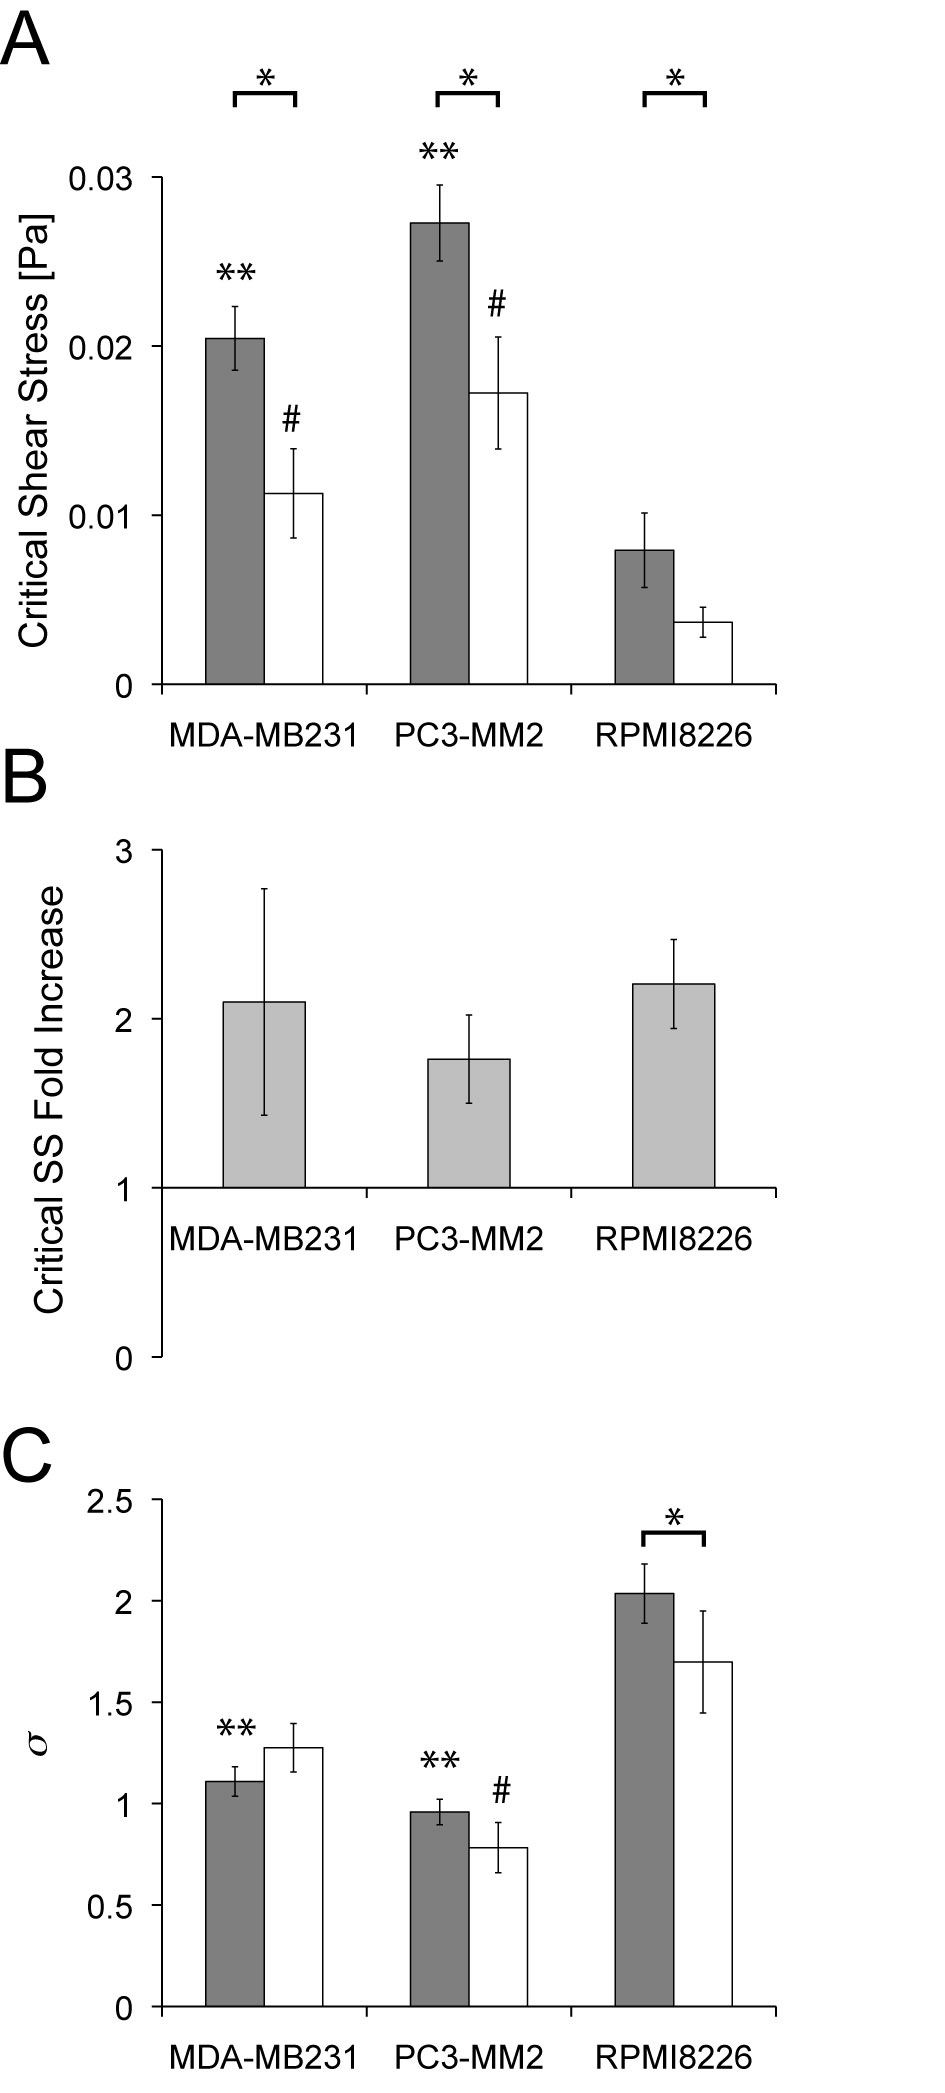
\includegraphics[height=6in]{Figure_FinalGraphs.jpg}
\caption{\textbf{Comparison of adhesion to a HUVEC monolayer}. (A) Average critical shear-stress on activated (gray bars) and non-activated (white bars) endothelium. (B) Average fold increase in critical shear-stress. (C) Average $\sigma$ of lognormal distribution on activated (gray bars) and non-activated (white bars) endothelium. $\ast: P < 0.05$ for combined block multiple experiments between activated and non-activated endothelium for given cell type. $\ast\ast: P < 0.05$ compared to RPMI8226 on activated endothelium.  $\#: P < 0.05$ compared to RPMI8226 non-activated endothelium.}
\label{Chap:TumorCellAdhesion:fig:summaryGraphs}
\end{figure}

Fitted values of $\sigma$ were also compared between non-activated and activated endothelium groups and  across cell types. No statistically significant differences were found between activated and non-activated endothelium conditions for comparisons within each cell type (Figure \ref{Chap:TumorCellAdhesion:fig:summaryGraphs}C). However, $\sigma$ values for RPMI8226 cells were significantly higher than those for PC3-MM2 and MDA-MB231 for both activated and non-activated endothelium groups. These data suggested that $\sigma$, which represents the heterogeneity in cell adhesion of the population, was not influenced by endothelial activation, but only by intrinsic differences between cells. 

Collectively, the pair of fitted parameters $\tau_{50}$ and $\sigma$ have revealed expected yet nevertheless interesting similarities and differences between the cancer cell types, which can be interpreted as follows. No difference in the heterogeneity of the metastatic breast and prostate cancer cell line adhesion could be observed and this heterogeneity did not change significantly upon activation of the endothelium. That is to say, although endothelial activation enhanced adhesion for these two cell types, the level of enhancement was consistent across all individual cells within the population (i.e., no change in spread in the LNcdf was observed), and consistent across cell types (\ie, no significant change in the fold-increase of $\tau_{50}$ was observed either). RPMI8226 cells were similarly affected by endothelial activation, but in comparison to PC3-MM2 and MDA-MB231 cells, RPMI8226 cells were much less adherent and displayed much more heterogeneity in the population. This heterogeneity is potentially related to its low adherence, since loose adhesion from non-specific interactions is likely to yield low $\tau_{50}$ and high $\sigma$. 

\section{Conclusion}
A novel approach for examining cell attachment has been presented that integrates a unique method for producing oscillatory flow, high resolution sweep of shear-stress, fully automated image analysis algorithm, and comprehensive examination of population heterogeneity. The sensitivity and repeatability of the method was validated by confirming an increase in adhesion of three different tumor cell lines representing 3 different cancers to a HUVEC monolayer upon activation of the monolayer using IL-1$\beta$. Unique insight into population heterogeneity was enabled by the use of oscillatory flow. The use of oscillatory flow also enabled the use of passive-pumping to allow samples to be loaded and treated using a pipette. Thus, the platform enables complete separation of microchannels to ensure independence of each data point acquired in the array. Taken together, the method presented here offers new insight into cell adhesion, represents a significant advance to the study of cell attachment, and has the potential to advance our understanding of adhesion in areas such as cancer metastasis, inflammation, and regenerative medicine.

\section{Materials and Methods}

\subsection{Cell Culture}

Human umbilical vein endothelial cells (HUVECs) were purchased from Lonza (Walkersville, MD), and regularly cultured on tissue culture-treated flasks pre-coated with 1.5 $\mu$g/cm$^2$ of bovine plasma fibronectin (FN) (Sigma-Aldrich, St. Louis, MO). HUVECs were maintained in EGM BulletKit media (CC-3124, Lonza) consisting of EBM-2 basal medium supplemented with 2\% fetal bovine serum (FBS), bovine brain extract with heparin, hEGF, hydrocortisone, and gentamicin/Amphotericin B. HUVECs were fed every other day, passaged every 3-4 days at 90\% confluence, and only passages 4-6 were used in microchannel experiments. 

To prepare HUVEC monolayers for adhesion tests, microchannels were first primed with 30 $\mu$L PBS followed by 20 $\mu$L FN at 100 $\mu$g/mL concentration. Microchannels were incubated at 37 deg C for 1 h in humidified trays to allow FN adsorption to the microchannel walls. After incubation, FN was replaced twice with 40 $\mu$L HUVEC media further supplemented with 10 mM HEPES. HUVECs were seeded at 3000 cells/$\mu$L $\times$ 6 $\mu$L per microchannel, and allowed to adhere and culture overnight (12 h). HUVEC microscale cultures were either used on the same day for adhesion tests if confluent, or maintained for an additional day to reach full confluence. Activated HUVEC monolayers in microchannels were induced with 10 $\mu$g/mL interleukin-1$\beta$ (IL-1$\beta$) for 4 h before adhesion tests.

Three different human cancer cell lines were used in adhesion tests to compare adhesion strengths on activated versus non-activated endothelium. MDA-MB231 cells (mammary gland epithelial) were maintained in DMEM with 4.5 g/L glucose supplemented with 10\% FBS and 1\% penicillin/streptomycin (P/S). PC-3 MM2 cells (metastatic prostate) were maintained in RPMI1640 with L-glutamine, 10\% FBS, 1\% penicillin/streptomycin (P/S), and 10 mM HEPES. RPMI8226 cells (multiple myeloma in bone marrow) were maintained in DMEM with 4.5 g/L glucose supplemented with 10\% FBS, 1\% P/S, and 10 mM HEPES.  MDA-MB231 and PC3-MM2 cells were fed every other day and passaged every 3-4 days depending on confluence. RPMI8226 cells were passaged every 3 days. All cell lines were resuspended at 1000-1500 cells/$\mu$L, and 7.5 $\mu$L of cell suspension was dispensed into each microchannel. Thus, each microchannel contained approx. 7,500 to 12,000 cells.

\subsection{Immunostaining and HUVEC activation}

Immunostaining was performed to verify upregulation of E-selectin upon activation using IL-1$\beta$. Fig \ref{Chap:TumorCellAdhesion:fig:staining} shows that E-selectin upregulation was robust for all concentrations tested while the control showed basal levels. Acquisition parameters were identical and images were treated uniformly.

\begin{figure}[!ht]
\centering
\includegraphics[width=3.5in]{StainingImages.pdf}
\caption{\textbf{HUVEC staining for E-selectin}. Concentration of IL-1$\beta$ is indicated in the corner of each image.}
\label{Chap:TumorCellAdhesion:fig:staining}
\end{figure}


\subsection{Image Capture and Analysis}

Prior to data acquisition, a calibration procedure described in Chapter \ref{Chap:Oscillator} was used to measure the initial shear stress of the system at 140 mV piezo voltage and 2 Hz sinusoidal oscillation frequency. The actuator was perturbed by gentle tapping to redistribute cells within the field of view that moved due to the calibration procedure. After waiting 30 seconds for cells to settle, the acquisition protocol was started.

Data acquisition consists of 41 stream acquisitions. The first 5 are to be acquired at 2 Hz. At the start of the sixth stream, a descending log frequency sweep is begun that lasts for 500 s and ends at 0.1 Hz. The first six datapoints obtained at a frequency of 2 Hz are used to normalize each curve. The average of those six measurements is forced to a value of one resulting in a proportional adjustment of all other values.

MetaMorph was used to acquire the image streams at specified intervals of time using the journaling capability of the software. The software also allows for the logging of times. The time at the beginning of each image stream is recorded to allow back-calculation of the frequency. This is helps improve accuracy because MetaMorph is not able to perform each stream acquisition at precisely the same time for each channel due to variability in data read-write times. The number of frames per stream was chosen to ensure capture of 1-2 cycles of fluid\slash cell motion and ranged from 25 to 170. Variable numbers of frames were used to limit the amount of data.

Images were acquired at 2X with a binning of 2 $\times$ 2 and an exposure time of 15 ms. The Ph1/PhC phase rings were used to provide maximal contrast (\ie, dark background and bright cells).

\subsection{Statistical Analyses}

\paragraph{Effects of activation.} Median $\tau_{50}$ and standard deviation $\sigma$ were determined from the lognormal curve fits for each condition (HUVEC activation and cell type), and statistically compared using nonparametric tests. First, to determine whether activation of HUVEC monolayers via IL-1beta induction had an effect on cell adhesion for each cell type, we used a combined Wilcoxon rank sum approach proposed by Lehmann (1998) for handling the complete data set consisting of multiple experiments with varying sample sizes. This required that we group our data into blocks for the separate experiments, with each block consisting of $m$ activated and $n$ non-activated monolayers.

\paragraph{Differences between cell type.} Independent Kruskal-Wallis tests were used to determine whether differences in $\tau_{50}$ and $\sigma$ were present across cell types for both the activated and non-activated monolayers. We further normalized $tau_{50}$ by defining the ratio or ``fold-increase'' of activated to non-activated adhesion, and performed Kruskal-Wallis analysis on normalized $tau_{50}$. All Kruskal-Wallis tests were performed on values averaged across samples in the same experiment.

When Kruskal-Wallis tests revealed significant differences in the data, post hoc multiple comparison tests were performed via independent Wilcoxon rank-sum tests, with and without Bonferroni correction, between separate pairs of cell types to determine which cell types differed from the others. 

\paragraph{Outliers.} Coefficients of determination ($R^{2}$) were calculated for each curve fit, and it was found that $R^{2}$ = 0.94 +/- 0.06 for the fifty experiments we conducted. One outlier was detected ($R^{2}$ = 0.60), and removal of the outlier resulted in $R^{2}$ = 0.95 +/- 0.04. The above statistical tests were done with both inclusion and exclusion of the outlier, and it was found that the main conclusions were not affected by the presence of the outlier.





\chapter{Assays: Cell Adhesion Assay Validation: Tumor-Cell Adhesion to a HUVEC Monolayer}
\label{Chap:TumorCellAdhesion}

\section{Preface}
This work was performed and written in equal collaboration with Edmond Young as represents a manuscript in preparation.

\section{Introduction}
The process of cell adhesion involves physical interactions between cells and the materials in their microenvironment such as extracellular matrices, synthetic biomaterial surfaces, and other cells and is a major topic of interest in areas ranging from fundamental cell biology and pathophysiology \cite{Chen:1997p320,Davies:1995p87} to tissue engineering and regeneration \cite{Nugent:2003p459}. In particular, cell adhesion plays an integral role in inflammation and cancer metastasis where leukocytes and circulating neoplastic cells, respectively, interact with the vascular endothelium in complex adhesion cascades that include tethering, rolling, spreading and endothelial transmigration events \cite{Ley:2007fk,Geiger:2009vn}. The ability to examine and measure the propensity of cells to adhere to the endothelium or other surfaces (engineered or natural) and determine the strength of adhesion is thus critically important to advancing our understanding of the mechanisms related to inflammation and cancer and to the development of tissue engineering strategies in regenerative medicine.

While cell adhesion fundamentally relies on the biophysical and biochemical properties of individual cells \cite{Orsello:2001uq}, many adhesion studies use population-based assays to determine global adhesion characteristics that efficiently reveal important and relevant properties of the cell population \cite{Christ:2010ly}. Population-based adhesion assays typically depend on fluid-flow systems that generate mechanical shear-stress, providing means to promote or challenge adhesion to the substrate on interest in a controlled manner. The most common fluid-flow systems for studying cell adhesion include the parallel-plate flow chamber \cite{GIAVAZZI:1993ty}, radial flow chamber \cite{Goldstein:2002p106}, cone-and-plate viscometer \cite{Jadhav:2001ys}, variable width devices \cite{Heilshorn:2003ly,Usami:1993p603}, and variable-height chambers \cite{Xiao:1996p618}. These systems typically employ steady flow conditions, but they can also be readily modified to accommodate oscillatory or pulsatile flow conditions for studies in shear-mediated atherosclerosis and cardiovascular pathobiology \cite{KU:1985uq,Chappell:1998fk}. Depending on the purpose of the study and availability of resources, flow systems can be operated under various schemes or protocols to produce different types of adhesion assays. For example, flow-rate\slash shear-stress can either be increased or decreased in a stepwise fashion to assay the gradual detachment or attachment of cells, respectively. Furthermore, shear-stress ranges can be expanded, or the number of steps in the ramping scheme can be increased to yield a more continuous scheme with better resolution for detecting adhesion events than more discrete protocols. Although fluid-flow systems have become indispensable tools in biological research, these systems have significant drawbacks due to their large scale, complex setup, and need for large volumes of medium and cell suspension to maintain flow. 

Recently, a number of microfluidic systems have been developed for cell adhesion and shear-flow assays \cite{Lu:2004ys,Gutierrez:2007p290,Plouffe:2007p274,Young:2007ml}, taking advantage of microfabrication techniques to create systems that can increase throughput, handle reduced fluid volumes, and improve spatiotemporal control of \invitro\ microenvironments \cite{Young:2010p286,Young:2010uq}. While these microscale flow systems have shown improvements over their macroscale counterparts and have overcome some of the main drawbacks of previous systems, the majority of microfluidic systems continue to require complex ``world-to-chip'' interfacing \cite{Fredrickson:2004ve} that limits their potential for widespread adoption in biology labs, particularly in clinical and translational research applications where limited patient-derived cell and tissue samples may be significantly depleted by excessive tubing and large dead volumes. 

We have developed a novel microscale system for conducting oscillatory, shear adhesion assays that employs passive-pumping principles to eliminate cumbersome interconnects and unnecessary tubes and dead volume. The system, described in detail below, enables pipette-based loading and treatments, is easily amenable to complex microscale geometries, and can be dynamically controlled to offer various oscillatory waveforms for cardiovascular applications. Most importantly, this microscale system offers analysis of the adherence of a small and defined population of cells in a manner that cannot be achieved with existing systems, thus enabling studies of limited cell samples such as those acquired from a clinical setting. These capabilities, coupled with a custom information-rich readout, allow this system to be applied to a wide range of biological experiments. To illustrate the potential of this system and custom readout, we developed an attachment-based adhesion assay that utilizes a decreasing log-sweep of shear-stress and differential image analysis of image-streams to quantify the process of adhesion for an entire population of interest. We used the integrated system to study adhesion of three different cancer cell-lines on activated and non-activated endothelial monolayers. Results demonstrate the ability of this approach to provide new insights into the heterogeneity of cell populations and adhesion mechanisms.

\section{Results and Discussion}

\subsection{System Design and Operation}

Our main objective was to design, test, and implement a passive-pumping-based oscillatory flow system for an array of microchannels in order to extend oscillatory modes of shear flow to pipette friendly systems.  Passive-pumping has been used previously in various applications, and has been described in detail elsewhere \cite{Berthier:2007mi,Meyvantsson:2008,Walker:2004ov}. Briefly, passive-pumping leverages surface tension to pump fluid from small droplets to larger droplets based on Laplace's law (Figure \ref{figure:schematic}A). We fabricated a simple one-input-one-output straight microchannel where one port is smaller than the other to facilitate passive-pumping of cell suspensions, media, and reagents. To generate oscillatory flow, we further designed and fabricated a diaphragm from polydimethylsiloxane (PDMS) that was positioned over the larger outlet port and reversibly sealed to the top of the PDMS microchannel. The diaphragm was actuated using a piezoelectric cantilever which bends in response to a voltage signal. The actuator was retrofitted with an adjustable cap screw to provide a single point of contact between the actuator and diaphragm (Figure \ref{figure:schematic}B). Voltage signals were produced using a function generator and passed through an amplifier to the actuator to tunably control displacement of the cap screw tip. The resulting deflections of the diaphragm induce pressure changes within the sealed air chamber below the diaphragm to drive oscillatory flow within the microchannel. The ports act as reservoirs for volume fluctuations with the exposed port providing pipette access to deliver treatments or cell suspension.

\begin{figure}[ht] %DONE
\centering
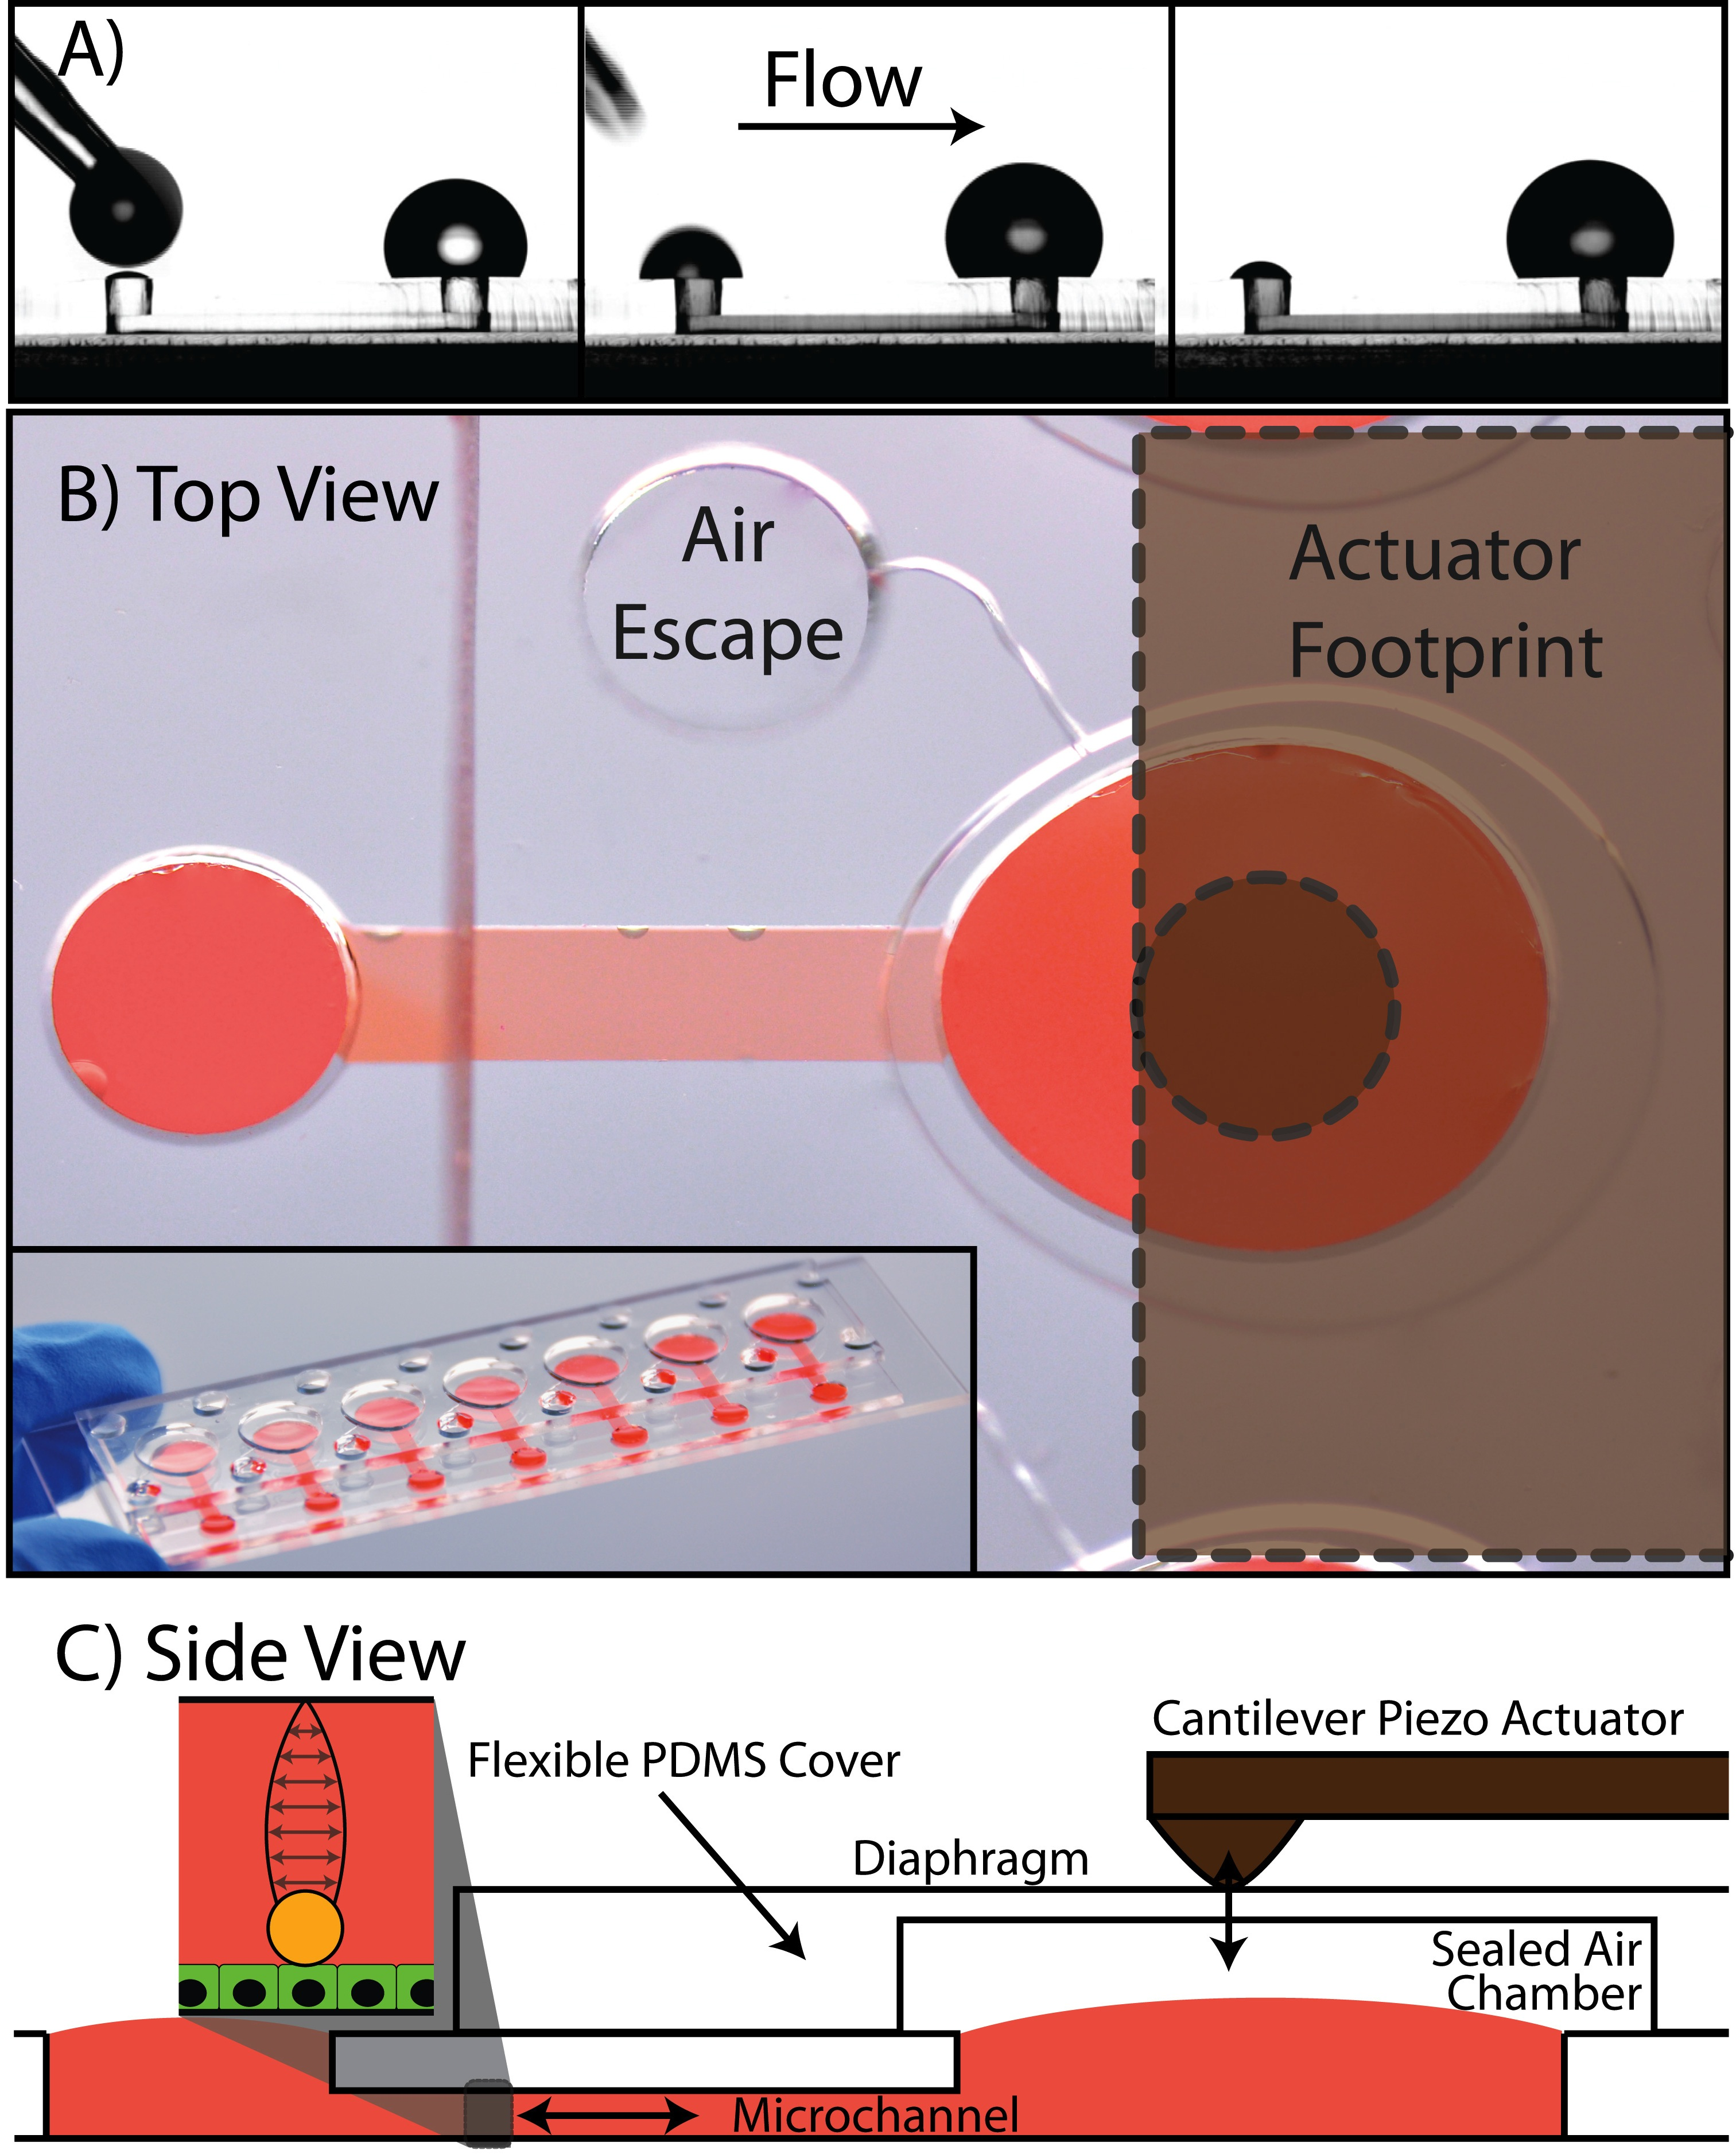
\includegraphics[width=3.5in]{OscillatoryDiagram4.jpg}
\caption{\textbf{Oscillatory flow device}. (A) Side images of passive pumping via dispensed droplets. (B) Top view of microchannel and diaphragm assembly. Inset shows 7 x 1 array of microchannels on a single microscope slide. (C) Side view of setup. Cantilever piezoelectric actuator deflects diaphragm according to applied voltage signals. At low frequency and moderate amplitude, this creates a volume change in the air cavity and displaces fluid in the channel. Oscillatory shear-stresses may be generated with this approach, allowing it to be used for various cell adhesion studies.}
\label{figure:schematic}
\end{figure}

The dimensions of the straight microchannel mimic the dimensions of a conventional parallel-plate flow chamber while the microchannel ports provide the ability to load and treat cells via pipette. The use of microfabrication techniques will allow us to rapidly explore more complex designs in the future. The footprint of the device provides a modest increase in throughput, i.e., up to seven microchannels per array during one microscope acquisition session, but perhaps more importantly, the microchannels were independently addressable. Maintaining separation ensures that each endothelial monolayer is cultured, activated, and\slash or mechanically stimulated as independent biological samples without adverse cross-talk, as is the case in many multiplexed microfluidic systems. In co-culture adhesion studies, this property has the potential for an even larger impact: the system can test limited cell samples, such as those acquired from clinical patients, as demonstrated by our use of $\sim 10^4$ cells per channel. This is a relatively small amount of cells compared to $\sim 10^6$ to $10^7$ cells typically needed for large-scale (mL) continuous flow in parallel-plate flow chambers. We envision that the system can be scaled if necessary to take even fewer cells ($10^2$ or $10^3$ cells), with only minor modifications to microchannel dimensions.

The oscillatory flow methods used here also have potential utility in other biological applications such as cardiovascular and bone mechanobiology, where oscillatory shear-stress has been implicated in important regulatory functions. Macroscale oscillatory flow systems have already been accepted into the laboratory setting while microscale oscillatory systems (and recirculatory systems in general) have also begun to appear \cite{Song:2005p157,Shao:2009p534}; however, the current design is the first oscillatory system to employ passive-pumping, thus combining the advantages of microscale approaches with simple pipette-based operation that obviate the need for tubing that inherently leads to excess dead volume.

The most innovative features of the demonstrated method are the integrated use of the piezoelectric actuator-PDMS membrane, and the development of a unique cell adhesion readout that has potential to offer new biological insights into cell adhesion phenomena. We leveraged the elastic properties of PDMS to create a sealed air chamber and diaphragm with negligible damping effects below 30 Hz and moderate amplitudes. However, oscillatory flow in a microchannel of these dimensions produces non-linear shear-stress response above 5 Hz. Above 5 Hz, the flow profile becomes non-parabolic. Above 30 Hz, the compliance of the air chamber results in significant attenuation of shear-stress. However, a property of laminar flow (steady and pulsatile) is that shear-stress at a given frequency is always linear to the pressure gradient. Clearance between the diaphragm and fluid in the port also limits actuator amplitudes. However, only 30 \textmu m of motion is required to produce the maximum shear-stress used in this study. As mentioned earlier, the microchannel ports act as reservoirs for oscillatory fluid exchange and thus limit the total volume that can be exchanged between the ports per cycle. The adhesion studies to date have been done in the low frequency regime where damping is insignificant leading to a linear relationship between frequency and shear-stress.

\subsection{Adhesion Assay via Image Differencing}

\paragraph{Measurement of Attachment \vs\ Detachment.}The use of a piezoelectric actuator enables the use of a wide variety of signal waveforms and flexible control of the shear-stress protocol. This capability allowed us to develop an 8-minute adhesion assay that samples a large range of frequencies at high resolution using a logarithmic sweep that spans two orders of magnitude (2 Hz to 100 mHz). Thus, this system provides similar resolution to that presented recently by \cite{Christophis:2010fk}. However, in contrast to Christophis \etal\ and other assays that ramp up shear-stress to detect detachment events, we have employed an inverse strategy where cells are initially prevented from adhering by starting at a relatively high shear-stress and then gradually \emph{reducing} shear-stress in order to monitor the \emph{attachment} events instead of \emph{detachment}.

\paragraph{Oscillatory \vs\ Flow-Through Methodologies}Although both oscillatory and flow-through devices can be used to study both attachment and detachment, the use of oscillatory flow fundamentally changes the readout of an attachment assay compared to flow-through devices and provides new insights into adhesion properties that have not been previously obtained. The \emph{attachment} readout of the oscillatory adhesion assay is identical to the \emph{detachment} readout reported by Christophis \etal. In the case of Christophis \etal\, the population of interest is completely defined prior to detachment, enabling them to present detachment results over a range of shear-stresses in terms of ``\% of the entire population of interest''. In doing so, they are able to directly measure the shape of the population distribution with respect to detachment shear-stress. The ability to measure the shape of the population distribution can provide important insight into the mechanisms of adhesion. In our case, the population of interest can also be defined as those cells that are initially in the field-of-view. The oscillatory nature of the flow allows us to monitor this population of interest over time for different levels of shear-stress to report the number of adhered cells as a \% of the entire population at various shear-stresses, thereby directly measuring the shape of the population distribution as well. This is different from other attachment assays that used flow-through or recirculation devices. When flow-through devices (\eg, the Christophis \etal\ device) are used in ``attachment-mode'' it becomes more difficult to define what an entire population is and makes it much more challenging to elucidate the shape of the population distribution. Thus, it is the oscillatory nature of the flow that enables a direct measurement of population distributions for attachment assays.

A previous study by Wang \etal\ used pulsing flow to study cell attachment and leveraged the ability to follow a single cell over time to examine individual attachment events; however, shear-stress in the system is uncharacterized and the readout was not extended to provide information regarding the distribution of the population \cite{Wang:2009kl}. The embodiment also differs significantly from that reported here given the use of tubes and a mechanical pumping mechanism with limited flexibility for defining complex flow patterns. Also, the study used image streams and image differencing to obtain measurements of \emph{cell motion} which were then normalized using knowledge of cell densities and suspension volumes to compare relative amounts of adhesion between two different cell populations at a given shear-stress. Here, a fully automated algorithm uses image difference information to directly measure the percent of cells adhered for an entire population over a range of shear-stresses.

\paragraph{Image Analysis: Preprocessing.}The percent of adhered cells is determined using phase-contrast microscopy. The data set for each channel consists of 41 image streams, each containing 25-170 images depending on the length of time needed to acquire 1-2 cycles of cell motion. The background is subtracted from all the images in the data set. The image used for background subtraction is determined from the first stream of images. In phase contrast using low magnification (2X), the cells appear brighter than the background. Thus, a stack projection is performed on the first stream to determine the minimum intensity for each pixel over time, removing any brighter moving objects (\ie, suspended cells) from the resulting background image. Thus, the background subtracted images in the data set are greatly enhanced to show suspended cells that were added to the channel. By using the same background image to perform all background subtraction for a given channel, any suspeded cells that adhere at a later time-point will still show up as being bright. An Otsu automatic thresholding routine is used to threshold the enhanced images to produce binary images with cells appearing white and background black. The background subtraction process produces stark contrast between the cells and background to make the automatic thresholding routine very robust. A single region of interest (ROI) is then chosen and applied to all images of the data set to restrict analysis from considering portions of the image where no cells exist and where shear-stress is uniform. Given the channel dimensions used in this study, the center 80\% of the channel width exhibits uniform shear-stress and is chosen using the ROI. All subsequent analysis is limited to this ROI.
 
\paragraph{Image Analysis: Quantifying the Percent of Adhered Cells.}Fig \ref{Chap:TumorCellAdhesion:fig:differencing} shows an idealized version of the black and white image streams that result from preprocessing and helps to describe the algorithm used to determine the percent of cells adhered to the substrate. In any given frame of a stream, there can be adhered (A) and non-adhered (NA) cells. In a different frame of the same series, non-adhered cells show up in a different location whereas adhered cells remain in the same spot. Thus, if we take the absolute difference of these two frames the non-adhered cell will show up twice whereas the adhered cell will show up once. Depending on the frames that are chosen, the impressions of the non-adhered cell may partially overlap.

\begin{figure}[!bt]
\centering
\includegraphics[width=6in]{ImageDifferencing.pdf}
\caption{\textbf{Image differencing algorithm}. $F_{n}$ refers to the $n^{th}$ frame of a time-series of images. $F_{n+\Delta n}$ refers an image taken $\Delta n$ frames after $F_{n}$. NA refers to a cell that is \underline{n}ot \underline{a}dhered where as A refers to a cell that is \underline{a}dhered.}
\label{Chap:TumorCellAdhesion:fig:differencing}
\end{figure}

If the impressions do not overlap then Eq \ref{Chap:TumorCellAdhesion:equ:percentAdhered} can be used to predict the percent of cells adhered where $F_{i}$ represents the integrated intensity of the $i^{th}$ binary image. For each stream the reference frame $F_{n}$ is chosen as the frame which exhibits the most average intensity over the course of the stream. The quantity $\left| F_{n}-F_{n+\Delta n}\right|$ is then calculated for all other images while holding $F_{n}$ constant. Partial overlap reduces the value of $\left| F_{n}-F_{n+\Delta n}\right|$ and is expected to occur less than 30\% of the time given our number of frames and minimum cell amplitudes. Therefore the top 5\% of these values are averaged to potentially reduce noise in determining a final value for the numerator of Eq \ref{Chap:TumorCellAdhesion:equ:percentAdhered}. This number is proportional to twice the number of non-adhered cells whereas $F_{n}$ is proportional to the number of total cells, thus arriving at Eq \ref{Chap:TumorCellAdhesion:equ:percentAdhered} for the percent of adhered cells. This process is repeated for each of 41 streams in the data set for each channel to produce a plot of `\% of Population Adhered' \vs\ `Shear-Stress'. It is possible that if oscillation and image acquisition were synchronized, image streams would no longer be necessary as a good choice for $F_{n}$ and $F_{n+\Delta N}$ can be predicted based on the sinusoidal nature of the oscillation.

\begin{equation}
\textrm{\% of Pop. Adhered} = 1 - \frac{\left| F_{n}-F_{n+\Delta n}\right|}{2 \, F_{n}}
\label{Chap:TumorCellAdhesion:equ:percentAdhered}
\end{equation}

\paragraph{Batch Processing.}The image filtering and analysis is completely automated using custom software called Je'Xperiment, developed by Jay Warrick and Erwin Berthier at the University of Wisconsin Madison. The software is used to database the images and perform batch processing of the custom algorithm. One array of 7 channels produces approximately 10-15 gigabytes of data. The primary time constraint of the analysis is thus the time it takes to read and write the images to a hard drive or server ($\sim$ 5 hours total). However, Je'Xperiment allows one to obtain results with less than 10 minutes of time actually invested by the user at the computer workstation.

\paragraph{Interpretation of Results.}Fig \ref{Chap:TumorCellAdhesion:fig:logNorm} illustrates the shape of the resulting adhesion plot and the log-normal cumulative distribution function (LNcdf) used to fit the data. The LNcdf (Eq \ref{Chap:TumorCellAdhesion:equ:LNcdf}) has two parameters, $\mu$ and $\sigma$, which are obtained from the curve fit. The quantity $e^{\mu}$ represents the median shear-stress of the population, $\tau_{50}$, whereas $\sigma$ indicates the spread, measured in orders of magnitude, of the data surrounding the median. This interpretation is different than a normal distribution where $\sigma$ gives an indication of absolute spread about the mean.

\begin{figure}[!t]
\centering
\includegraphics[width=3.5in]{TheoryPlot.pdf}
\caption{\textbf{Log-normal cumulative distribution function}.}
\label{Chap:TumorCellAdhesion:fig:logNorm}
\end{figure}

\begin{equation}
\textrm{LNcdf($x$,$\mu$,$\sigma$)} = \frac{1}{2} + \frac{1}{2}\textrm{erf}\left[ \frac{\ln{x} - \mu}{\sqrt{2 \sigma^{2}}}\right] 
\label{Chap:TumorCellAdhesion:equ:LNcdf}
\end{equation}

Interpretation of changes in the median are fairly straight forward but changes in $\sigma$ are less intuitive. For example, assume there is a cell type and a substrate that interact via one type of molecule with a median shear-stress of 1 Pa and has a $\sigma$ of 1 indicating that 97.89\% of all cells in the population adhere at a shear-stress between 0.1 and 10 Pa. In this idealized scenario, if the substrate is changed such that only 1/10$^{th}$ the original amount of adhesion ligand is presented to the cells, one would expect the median shear-stress to drop to roughly 0.1 Pa given that the number of anchor points per cell is lowered accordingly. Since each portion of the population would fall under this argument, shear-stress data would be predicted to simply shift while keeping $\sigma$ the same. That is to say, the new median shear-stress would be 0.1 Pa with 97.89\% of the population falling between 0.01 and 1 Pa.

On the other hand, what if the median does not change and $\sigma$ does? Given $\sigma$ is a measure of the heterogeneity of the interaction between the cells and substrate, a change in $\sigma$ indicates that the type of mechanism mediating adhesion (\ie\ the involvement of specific molecules or physical forces) has changed or has become more or less heterogeneous. However, it is more likely that multiple molecules or mechanisms mediate adhesion and contribute to an overall perceived heterogeneity. In this situation, if the influence of one of those contributing mechanisms were to be heightened, the value of $\sigma$ would change as well. If a single population has two dominant mechanisms of adhesion, it would result in the multiplication of two characteristic LNcdfs. On the other hand, if there are \emph{two} distinct populations, the result would be the renormalized addition of the two characteristic LNcdfs.

Thus, changes in $\sigma$ are associated with changes in the heterogeneity of the underlying mechanism, whereas changes in the median indicate changes in the strength or number of the interactions.

\subsection{Cancer cell adhesion}
Having defined the oscillatory attachment assay methodology, readout, and method of data interpretation; biological experiments are performed to characterize the sensitivity and repeatability of the assay for detecting physiologically relevant changes in adhesion interactions. We tested adhesion of three established cell lines derived from distinct types of cancer, including prostate (PC3-MM2), breast (MDA-MB231), and multiple myeloma (RPMI8226).  Studies on the adhesiveness, invasiveness and metastatic potential of these cell lines have shown that PC3-MM2 cells are particularly invasive among PC3 family of sublines \cite{Daja:2003rr}, and that PC3 sublines are highly variable in adhesiveness \cite{Dimitroff:2004bh}. MDA-MB231 cells are also highly invasive among breast cancer cell lines \cite{TOZEREN:1995wd,Lee:2003kx}, but are known to adhere to activated endothelium only in the absence of shear-stress $> 0.5$ dyn/cm$^2$ \cite{TOZEREN:1995wd}. In contrast to prostate and breast cancers, the adhesiveness and invasiveness of cells of multiple myeloma (MM) origin has been studied to a much lesser extent. Reports of MM cell adhesion that are available seem to suggest that adhesion to (bone marrow) endothelium is mediated by various molecules other than E-selectin \cite{Okada:1995ys,Broek:2008p301,Katz:2010uq}. Thus, we expected that PC3-MM2 and MDA-MB231 cells would exhibit more adhesive phenotypes, while RPMI8226 would likely show less adhesion to the endothelial monolayers.

We performed independent LNcdf curve fits for each condition, extracted the fitted $\tau_{50}$ and $\sigma$ values and compared results between activated and non-activated endothelium as well as across the different cell types. Fig \ref{Chap:TumorCellAdheison:fig:examples} shows examples of data and LNcdf fits for each cell type on activated and non-activated endothelium.

\begin{figure}[ht] %DONE
\centering
\begin{tabular}{cc}
A) PC3-MM2 & B) RPMI8226 \cr
\includegraphics[width=2.5in]{ExamplePC3.pdf} &\includegraphics[width=2.5in]{ExampleRPMI.pdf} \cr
C) MDA-231 & \cr
\includegraphics[width=2.5in]{ExampleMDA.pdf}
\end{tabular}
\caption{\textbf{Example adhesion curves for each condition}. Each pair of curves represents a adhesion measured in two channels on the same day. (blue) Non-activated endothelium. (red) Activated endothelium. }
\label{Chap:TumorCellAdheison:fig:examples}
\end{figure}

We observed statistically significant increases in $\tau_{50}$ (the critical shear-stress) between activated and non-activated endothelial surfaces for all cell types, including, surprisingly, RPMI8226 cells (Figure \ref{Chap:TumorCellAdhesion:fig:summaryGraphs}A). Comparing non-activated endothelium cases alone, both MDA-MB231 and PC3-MM2 cells exhibited significantly higher values of $\tau_{50}$ than RPMI8226 cells; this was also true for the activated endothelium cases alone, where MDA-MB231 and PC3-MM2 cells had higher $\tau_{50}$ than RPMI8226 cells (Figure \ref{Chap:TumorCellAdhesion:fig:summaryGraphs}A). Interestingly, when the \emph{ratio} between activated and non-activated $\tau_{50}$ values were calculated and compared, no difference was found between cell types (Figure \ref{Chap:TumorCellAdhesion:fig:summaryGraphs}B), suggesting that the effect of IL-1$\beta$ induction on adhesion was consistent across cell types. Thus, MDA-MB231 and PC3-MM2 cells were likely more adhesive than RPMI8226 cells because of intrinsic differences in cell surface properties, which were amplified for all cell types in the presence of E-selectin. This appeared to be consistent with the literature cited above.

\begin{figure}[!tb] %DONE
\centering
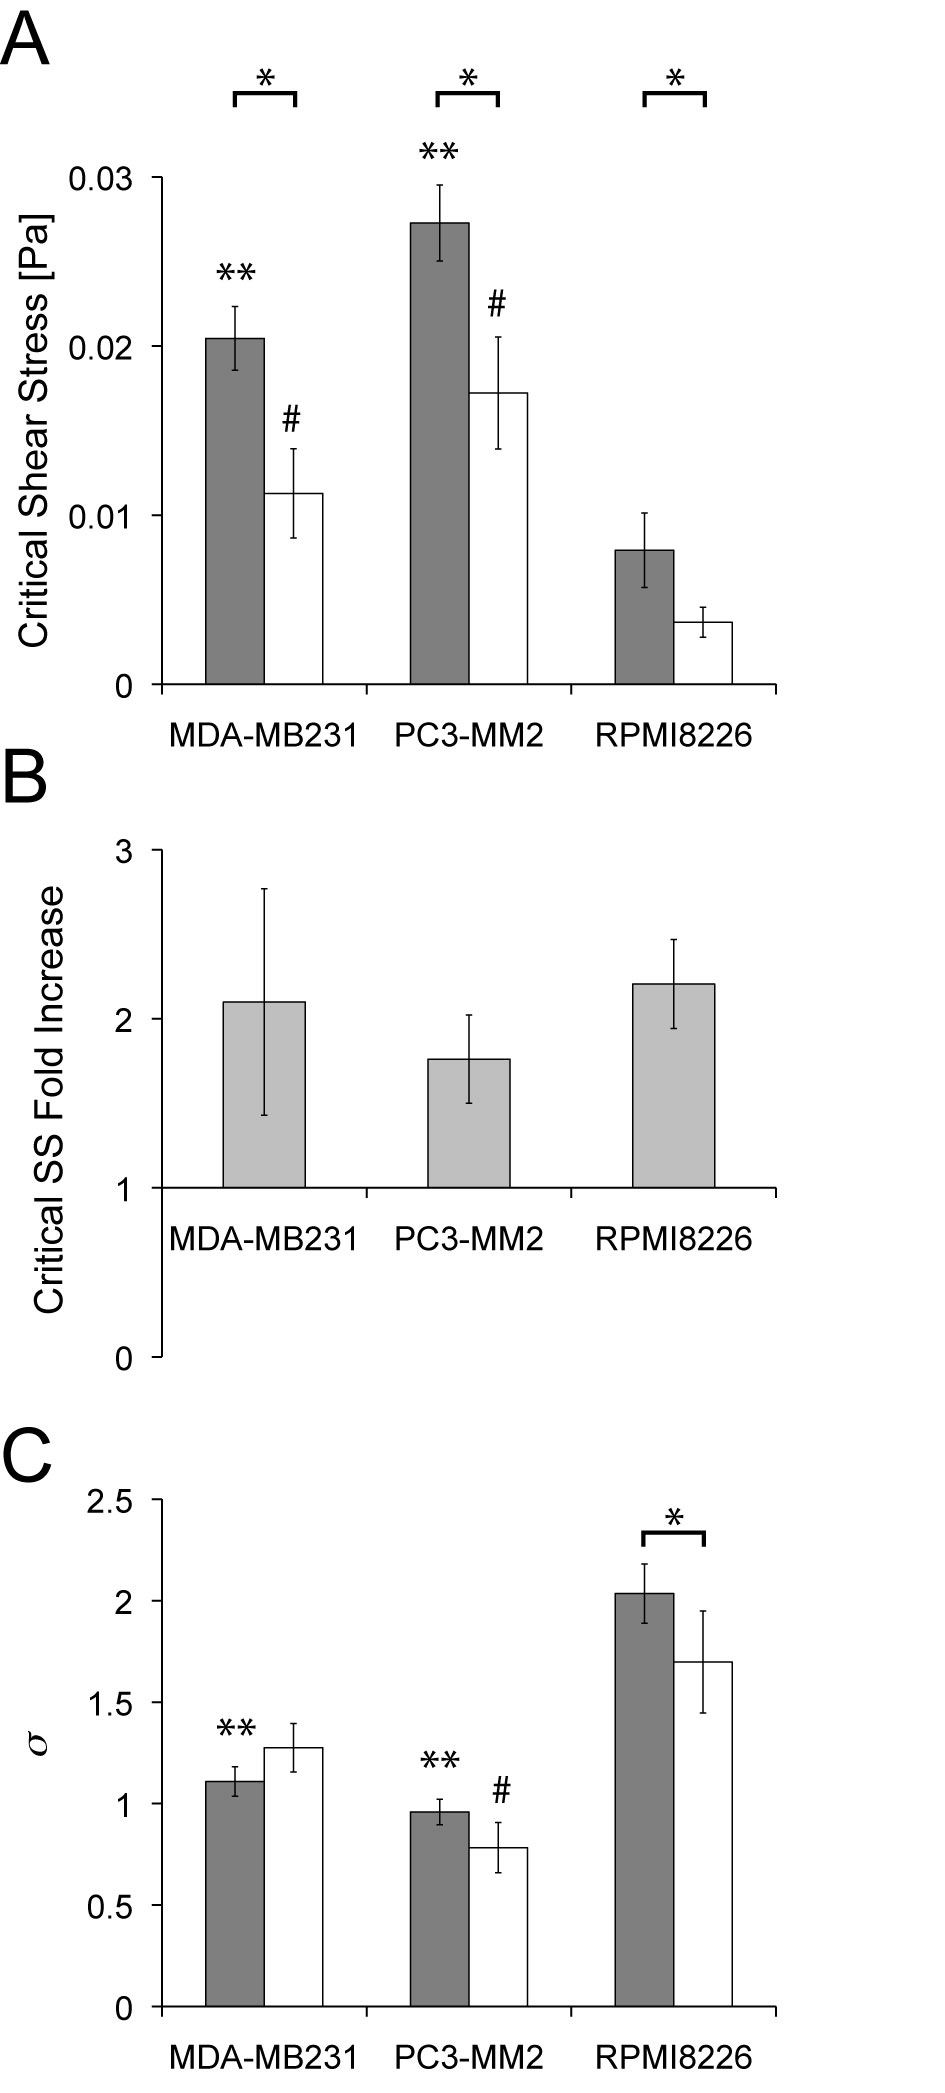
\includegraphics[height=6in]{Figure_FinalGraphs.jpg}
\caption{\textbf{Comparison of adhesion to a HUVEC monolayer}. (A) Average critical shear-stress on activated (gray bars) and non-activated (white bars) endothelium. (B) Average fold increase in critical shear-stress. (C) Average $\sigma$ of lognormal distribution on activated (gray bars) and non-activated (white bars) endothelium. $\ast: P < 0.05$ for combined block multiple experiments between activated and non-activated endothelium for given cell type. $\ast\ast: P < 0.05$ compared to RPMI8226 on activated endothelium.  $\#: P < 0.05$ compared to RPMI8226 non-activated endothelium.}
\label{Chap:TumorCellAdhesion:fig:summaryGraphs}
\end{figure}

Fitted values of $\sigma$ were also compared between non-activated and activated endothelium groups and  across cell types. No statistically significant differences were found between activated and non-activated endothelium conditions for comparisons within each cell type (Figure \ref{Chap:TumorCellAdhesion:fig:summaryGraphs}C). However, $\sigma$ values for RPMI8226 cells were significantly higher than those for PC3-MM2 and MDA-MB231 for both activated and non-activated endothelium groups. These data suggested that $\sigma$, which represents the heterogeneity in cell adhesion of the population, was not influenced by endothelial activation, but only by intrinsic differences between cells. 

Collectively, the pair of fitted parameters $\tau_{50}$ and $\sigma$ have revealed expected yet nevertheless interesting similarities and differences between the cancer cell types, which can be interpreted as follows. No difference in the heterogeneity of the metastatic breast and prostate cancer cell line adhesion could be observed and this heterogeneity did not change significantly upon activation of the endothelium. That is to say, although endothelial activation enhanced adhesion for these two cell types, the level of enhancement was consistent across all individual cells within the population (i.e., no change in spread in the LNcdf was observed), and consistent across cell types (\ie, no significant change in the fold-increase of $\tau_{50}$ was observed either). RPMI8226 cells were similarly affected by endothelial activation, but in comparison to PC3-MM2 and MDA-MB231 cells, RPMI8226 cells were much less adherent and displayed much more heterogeneity in the population. This heterogeneity is potentially related to its low adherence, since loose adhesion from non-specific interactions is likely to yield low $\tau_{50}$ and high $\sigma$. 

\section{Conclusion}
A novel approach for examining cell attachment has been presented that integrates a unique method for producing oscillatory flow, high resolution sweep of shear-stress, fully automated image analysis algorithm, and comprehensive examination of population heterogeneity. The sensitivity and repeatability of the method was validated by confirming an increase in adhesion of three different tumor cell lines representing 3 different cancers to a HUVEC monolayer upon activation of the monolayer using IL-1$\beta$. Unique insight into population heterogeneity was enabled by the use of oscillatory flow. The use of oscillatory flow also enabled the use of passive-pumping to allow samples to be loaded and treated using a pipette. Thus, the platform enables complete separation of microchannels to ensure independence of each data point acquired in the array. Taken together, the method presented here offers new insight into cell adhesion, represents a significant advance to the study of cell attachment, and has the potential to advance our understanding of adhesion in areas such as cancer metastasis, inflammation, and regenerative medicine.

\section{Materials and Methods}

\subsection{Cell Culture}

Human umbilical vein endothelial cells (HUVECs) were purchased from Lonza (Walkersville, MD), and regularly cultured on tissue culture-treated flasks pre-coated with 1.5 $\mu$g/cm$^2$ of bovine plasma fibronectin (FN) (Sigma-Aldrich, St. Louis, MO). HUVECs were maintained in EGM BulletKit media (CC-3124, Lonza) consisting of EBM-2 basal medium supplemented with 2\% fetal bovine serum (FBS), bovine brain extract with heparin, hEGF, hydrocortisone, and gentamicin/Amphotericin B. HUVECs were fed every other day, passaged every 3-4 days at 90\% confluence, and only passages 4-6 were used in microchannel experiments. 

To prepare HUVEC monolayers for adhesion tests, microchannels were first primed with 30 $\mu$L PBS followed by 20 $\mu$L FN at 100 $\mu$g/mL concentration. Microchannels were incubated at 37 deg C for 1 h in humidified trays to allow FN adsorption to the microchannel walls. After incubation, FN was replaced twice with 40 $\mu$L HUVEC media further supplemented with 10 mM HEPES. HUVECs were seeded at 3000 cells/$\mu$L $\times$ 6 $\mu$L per microchannel, and allowed to adhere and culture overnight (12 h). HUVEC microscale cultures were either used on the same day for adhesion tests if confluent, or maintained for an additional day to reach full confluence. Activated HUVEC monolayers in microchannels were induced with 10 $\mu$g/mL interleukin-1$\beta$ (IL-1$\beta$) for 4 h before adhesion tests.

Three different human cancer cell lines were used in adhesion tests to compare adhesion strengths on activated versus non-activated endothelium. MDA-MB231 cells (mammary gland epithelial) were maintained in DMEM with 4.5 g/L glucose supplemented with 10\% FBS and 1\% penicillin/streptomycin (P/S). PC-3 MM2 cells (metastatic prostate) were maintained in RPMI1640 with L-glutamine, 10\% FBS, 1\% penicillin/streptomycin (P/S), and 10 mM HEPES. RPMI8226 cells (multiple myeloma in bone marrow) were maintained in DMEM with 4.5 g/L glucose supplemented with 10\% FBS, 1\% P/S, and 10 mM HEPES.  MDA-MB231 and PC3-MM2 cells were fed every other day and passaged every 3-4 days depending on confluence. RPMI8226 cells were passaged every 3 days. All cell lines were resuspended at 1000-1500 cells/$\mu$L, and 7.5 $\mu$L of cell suspension was dispensed into each microchannel. Thus, each microchannel contained approx. 7,500 to 12,000 cells.

\subsection{Immunostaining and HUVEC activation}

Immunostaining was performed to verify upregulation of E-selectin upon activation using IL-1$\beta$. Fig \ref{Chap:TumorCellAdhesion:fig:staining} shows that E-selectin upregulation was robust for all concentrations tested while the control showed basal levels. Acquisition parameters were identical and images were treated uniformly.

\begin{figure}[!ht]
\centering
\includegraphics[width=3.5in]{StainingImages.pdf}
\caption{\textbf{HUVEC staining for E-selectin}. Concentration of IL-1$\beta$ is indicated in the corner of each image.}
\label{Chap:TumorCellAdhesion:fig:staining}
\end{figure}


\subsection{Image Capture and Analysis}

Prior to data acquisition, a calibration procedure described in Chapter \ref{Chap:Oscillator} was used to measure the initial shear stress of the system at 140 mV piezo voltage and 2 Hz sinusoidal oscillation frequency. The actuator was perturbed by gentle tapping to redistribute cells within the field of view that moved due to the calibration procedure. After waiting 30 seconds for cells to settle, the acquisition protocol was started.

Data acquisition consists of 41 stream acquisitions. The first 5 are to be acquired at 2 Hz. At the start of the sixth stream, a descending log frequency sweep is begun that lasts for 500 s and ends at 0.1 Hz. The first six datapoints obtained at a frequency of 2 Hz are used to normalize each curve. The average of those six measurements is forced to a value of one resulting in a proportional adjustment of all other values.

MetaMorph was used to acquire the image streams at specified intervals of time using the journaling capability of the software. The software also allows for the logging of times. The time at the beginning of each image stream is recorded to allow back-calculation of the frequency. This is helps improve accuracy because MetaMorph is not able to perform each stream acquisition at precisely the same time for each channel due to variability in data read-write times. The number of frames per stream was chosen to ensure capture of 1-2 cycles of fluid\slash cell motion and ranged from 25 to 170. Variable numbers of frames were used to limit the amount of data.

Images were acquired at 2X with a binning of 2 $\times$ 2 and an exposure time of 15 ms. The Ph1/PhC phase rings were used to provide maximal contrast (\ie, dark background and bright cells).

\subsection{Statistical Analyses}

\paragraph{Effects of activation.} Median $\tau_{50}$ and standard deviation $\sigma$ were determined from the lognormal curve fits for each condition (HUVEC activation and cell type), and statistically compared using nonparametric tests. First, to determine whether activation of HUVEC monolayers via IL-1beta induction had an effect on cell adhesion for each cell type, we used a combined Wilcoxon rank sum approach proposed by Lehmann (1998) for handling the complete data set consisting of multiple experiments with varying sample sizes. This required that we group our data into blocks for the separate experiments, with each block consisting of $m$ activated and $n$ non-activated monolayers.

\paragraph{Differences between cell type.} Independent Kruskal-Wallis tests were used to determine whether differences in $\tau_{50}$ and $\sigma$ were present across cell types for both the activated and non-activated monolayers. We further normalized $tau_{50}$ by defining the ratio or ``fold-increase'' of activated to non-activated adhesion, and performed Kruskal-Wallis analysis on normalized $tau_{50}$. All Kruskal-Wallis tests were performed on values averaged across samples in the same experiment.

When Kruskal-Wallis tests revealed significant differences in the data, post hoc multiple comparison tests were performed via independent Wilcoxon rank-sum tests, with and without Bonferroni correction, between separate pairs of cell types to determine which cell types differed from the others. 

\paragraph{Outliers.} Coefficients of determination ($R^{2}$) were calculated for each curve fit, and it was found that $R^{2}$ = 0.94 +/- 0.06 for the fifty experiments we conducted. One outlier was detected ($R^{2}$ = 0.60), and removal of the outlier resulted in $R^{2}$ = 0.95 +/- 0.04. The above statistical tests were done with both inclusion and exclusion of the outlier, and it was found that the main conclusions were not affected by the presence of the outlier.





%\chapter*{Conclusion}
%\addcontentsline{toc}{chapter}{Conclusion}
\chapter{Conclusion}
\label{Chap:conclusion}

Engineering for microfluidics for biological systems is not trivial. Engineers developing \invitro\ models have a lot of experience now and are capable of creating highly relevant constructs with many components that can be finely tuned to explore the biology of the model. A good design that enables new biology, faster biology or better biology should be embraced. Unfortunately, too many enabling technologies end up as a single publication in an engineering journal and sit in a wafer box on a shelf. One of the biggest hurtles in getting microfluidic platforms to achieve their full potential moving them into the hands of researchers who are capable of asking relevant, and impactful questions of them. The engineers who design these models have wondered why biologists are not lining up to get their hands on potential game-changing technologies, there's a sizable body of literature analyzing what engineers are doing wrong and how they can change to attract broader interest to their research. This document adds to that body of literature in hopes that something would stick and make microfluidic-enabled \invitro\ models somewhat more relevant to biologists. 


%% Start the appendices:
\appendix       % Chapters, sections are now appendix style
% \chapter{Droplet Geometry}
\label{App:DropletGeometry}

There are many different ways to formulate the geometry of passive pumping between an input drop and an output drop. The aim of this appendix is to describe the droplet geometry in as many ways as possible so that it does not need to be significantly re-derived in the future. The following variables are used.

\begin{table}[htdp]
\caption{\textbf{Droplet geometry variable names and definitions}. The subscript $i$ denotes the number of the droplet/port/wetted area of interest.}
\centering
\begin{tabular}{ll}\toprule
Variable&Description\cr
\midrule
$a_{i}$&Radius of the port/wetted area\cr
$R_{i}$&Radius of curvature of the droplet\cr
$\R_{i}$&$R_{i}/a_{i}$ (dimensionless)\cr
$H_{i}$&Height of the droplet\cr
$\h_{i}$&$H_{i}/a_{i}$ (dimensionless)\cr
$C_{i}$&Vertical position of the center of the radius of curvature of the droplet\cr
$\C_{i}$&$C_{i}/a_{i}$ (dimensionless)\cr
$V_{i,hemi}$&$\frac{2}{3}\pi a_{i}^{3}$\cr
$V_{i}$&Volume of the droplet\cr
$\V_{i}$&$V_{i}/V_{i,hemi}$ (dimensionless)\cr
$\theta_{i}$&Contact angle of the droplet with the device\cr

\bottomrule
\end{tabular}
\end{table}%

First we define relationships between the various variables of interest.

\section{\texorpdfstring{Radius of Curvature, $R_{i}$ and $\R_{i}$}{Radius of Curvature, Ri and Ri}}%%%%%%%%%%%%%%

\begin{equation}
%\centering
\R_{i}=\frac{R_{i}}{a_{i}}
\end{equation}

\begin{equation}
%\centering
\R_{i}=\sin^{-1}(\theta_{i})
\end{equation}

\begin{equation}
%\centering
\R_{i}=\frac{\h_{i}^{2}+1}{2\h_{i}}
\end{equation}

\section{\texorpdfstring{Height, $H_{i}$ and $\h_{i}$}{Height, Hi and Hi}}%%%%%%%%%%%%%%%%%%%%

\begin{equation}
%\centering
\h_{i}=\frac{H_{i}}{a_{i}}
\end{equation}

\begin{equation}
%\centering
\h_{i}=\frac{1-cos(\theta_{i})}{sin(\theta_{i})}=tan\left(\frac{\theta_{i}}{2}\right)
\end{equation}

\begin{equation}
%\centering
\footnote{always produces result between 0 and $a$}\:
\h_{i}=\R_{i}\left(1-\sqrt{1-\frac{1}{\R_{i}^{2}}}\right)
\end{equation}

\begin{equation}
%\centering
\h_{i}=\left(\frac{1-\left(-2\V_{i}+\sqrt{1+4\V_{i}^{2}}\right)^{2/3}}{\left(-2\V_{i}+\sqrt{1+4\V_{i}^{2}}\right)^{1/3}}\right)
\end{equation}

\section{\texorpdfstring{Contact Angle, $\theta_{i}$}{Contact Angle, theta}}%%%%%%%%%%%%%%%%%%%%

\begin{equation}
%\centering
\footnote{always produces result between 0\Deg and 90\Deg}\:
\theta_{i}=\arcsin\left(\frac{1}{\R_{i}}\right)
\end{equation}

\begin{equation}
%\centering
\theta_{i}=2\arctan\left(\h_{i}\right)
\end{equation}

\begin{equation}
%\centering
\theta_{i}=2\arctan\left(\frac{1-\left(-2\V_{i}+\sqrt{1+4\V_{i}^{2}}\right)^{2/3}}{\left(-2\V_{i}+\sqrt{1+4\V_{i}^{2}}\right)^{1/3}}\right)
\end{equation}

\section{\texorpdfstring{Volume, $V_{i}$ and $\V_{i}$}{Volume, Vi and Vi}}%%%%%%%%%%%%%%%%%%%

\begin{equation}
%\centering
\V_{i}=\frac{V_{i}}{V_{i,hemi}}
\end{equation}

\begin{equation}
%\centering
\V_{i}=\frac{1}{4}\h_{i}(3+\h_{i}^2)
\end{equation}

\footnote{always results in a normalized volume between 0 and 1 (\ie , $0\le V\le V_{hemi}$ or $0$\Deg$\le\theta\le90$\Deg)\label{fn:Vol}}
\begin{equation}
%\centering
\V_{i}=\frac{1}{4}\R_{i}\left(1-\sqrt{1-\frac{1}{\R_{i}^{2}}}\right)\left(3+\R_{i}^{2}\left(1-\sqrt{1-\frac{1}{\R_{i}^{2}}}\right)^{2}\right)
\label{equ:VofR1}
\end{equation}

\footnote{always results in a normalized volume $> 1$ (\ie , $V_{i,hemi}\le V_{i}\le\infty$ or $90$\Deg$\le\theta_{i}\le180$\Deg)}
\begin{equation}
%\centering
\V_{i}=2\R_{i}^3 - \frac{1}{4}\R_{i}\left(1-\sqrt{1-\frac{1}{\R_{i}^{2}}}\right)\left(3+\R_{i}^{2}\left(1-\sqrt{1-\frac{1}{\R_{i}^{2}}}\right)^{2}\right)
\label{equ:VofR2}
\end{equation}

$^{\ref{fn:Vol}}$
\begin{equation}
%\centering
\V_{i}=\frac{V_{i}}{V_{i,hemi}}=\frac{1}{4}\tan\left(\frac{\arcsin\left(\frac{a_{i}}{R_{i}}\right)}{2}\right)\left(3+{\tan\left(\frac{\arcsin\left(\frac{a_{i}}{R_{i}}\right)}{2}\right)}^{2}\right)
\label{equ:VofR3}
\end{equation}

$^{\ref{fn:Vol}}$
\begin{equation}
%\centering
\V_{i}=\frac{1}{4}\tan\left(\frac{\theta_{i}}{2}\right)\left(3+{\tan\left(\frac{\theta_{i}}{2}\right)}^{2}\right)
\end{equation}

\begin{figure}[!ht]
\centering
\includegraphics[width=3.2in]{Theta.pdf}
\caption{\textbf{Dimensionless variable relationships in passive pumping}. Plot of $a/R$ and contact angle, $\theta$, with respect to normalized droplet volume, $\V$ (or $V_{i}/V_{i,hemi}$). Theta is measured at the contact point between the spherical drop and the horizontal surface extending toward the center of the port.}
\end{figure}

\section{\texorpdfstring{Location of Center of Radius of Curvature, $C_{i}$ and $\C_{i}$}{Location of Center of Radius of Curvature, Ci and Ci}}

\begin{equation}
%\centering
\C_{i}=\frac{C_{i}}{a_{i}}
\end{equation}

\begin{equation}
%\centering
\C_{i}=\h_{i}-\R_{i}
\end{equation}

\begin{equation}
%\centering
\C_{i}=-\R_{i}\sqrt{1-\frac{1}{\R_{i}^{2}}}
\end{equation}

\begin{equation}
%\centering
\C_{i}=-\R_{i}\cos\left(\theta_{i}\right)
\end{equation}



% \chapter{Diffusion Modeling}
\label{App:Diffusion}

\section{PDGF Modeling}
The PDGF signaling parameters are taken from an analysis performed by Lauffenburger \etal\ \cite{Lauffenburger:1989fy}. The threshold sensing concentration is based on the dissociation constant of PDGF given as, K$_{d}$ = 10$^{-10}$ - 10$^{-9}$ [mol/L]. The production rate, q$_{PDGF}$, is given as 10$^{-16}$ - 10$^{-15}$ [g/cell/min] which was cited as being taken from Leof \etal\ \cite{LEOF:1986uq}, a study using human foreskin fibroblasts. The molecular weight was estimated to be 30 [kDa]. Using the molecular weight we can convert the units of q$_{PDGF}$ to yield 5e-16/(30000*60) = 2.78e-22 [mol/cell/s]. The Einstein-Stokes equation gives $D$ = 79 [\textmu m$^{2}$/s] for the 30 [kDa] molecule.

\section{EGF Modeling}
EGF modeling was taken from work by Knauer \etal \cite{KNAUER:1984fj} and Starbuck \etal \cite{STARBUCK:1992kl}. This work is based on data obtained using human and mouse fibroblasts. The EGF complex internalization rate constant, k$_{eC}$, was measured to be  5.3e-3 [s$^{-1}$]. Half maximal response occurs at 0.15 [ng/mL] and 2000 surface complexes per cell. This means an internalization rate of 2000*5.3e-3 = 10.6 [molecules/cell/s]. The molecular weight of EGF and the EGF\slash EGF binding protein complex were cited as 6.4 and 74 [kDa] respectively. Converting units we get a 10.6/6.022e23 = 1.76e-23 [mol/cell/s] EGF uptake rate for fibroblast cells. Thus, $q_{max}$ = 2*1.76e-23 = 3.52e-23 [mol/cell/s]. Cellular affinity for EGF is about 4.69e-11 [mol/L] vs. a K$_{d}$ of 4.7e-9 [mol/L]. Again, using the Einstein-Stokes equation, a 6.4 [kDa] molecule gives a diffusion coefficient of D = 131 [\textmu m$^{2}$/s] and 58 [\textmu m$^{2}$/s] for a 74 [kDa] molecule. The latter is used to estimate the diffusing protein.

Factor uptake, q, is assumed to follow the Michaelis-Menten kinetics with respect to the concentration of a rate limiting factor (Eq \ref{App:Diffusion:equ:uptakeRate}). The value $q_{max}$ represents the maximum uptake rate per cell. $C_{cb}$ is the concentration of factor at the cell boundary and $C_{th}$ is the Monod or Michaelis-Menten constant. Per the definition of the Michaelis-Menten constant (Eq \ref{App:Diffusion:equ:uptakeRate}), when $C_{cb} = C_{th}$ then $q = q_{max}/2$. Thus, we use the threshold sensing concentration for the Michaelis-Menten constant. Therefore, when concentration at the cell boundary is 0, there is no uptake of factor, while at $C_{th}$, uptake is $q_{max}/2$.

\begin{equation}
\label{App:Diffusion:equ:uptakeRate}
q = \frac{q_{max}C_{cb}} {C_{th}+C_{cb}} = \frac{q_{max}} {1+\frac{C_{th}}{C_{cb}}}
\end{equation}

%\section{Basic geometries}
%\begin{figure}[!t]
%\centering
%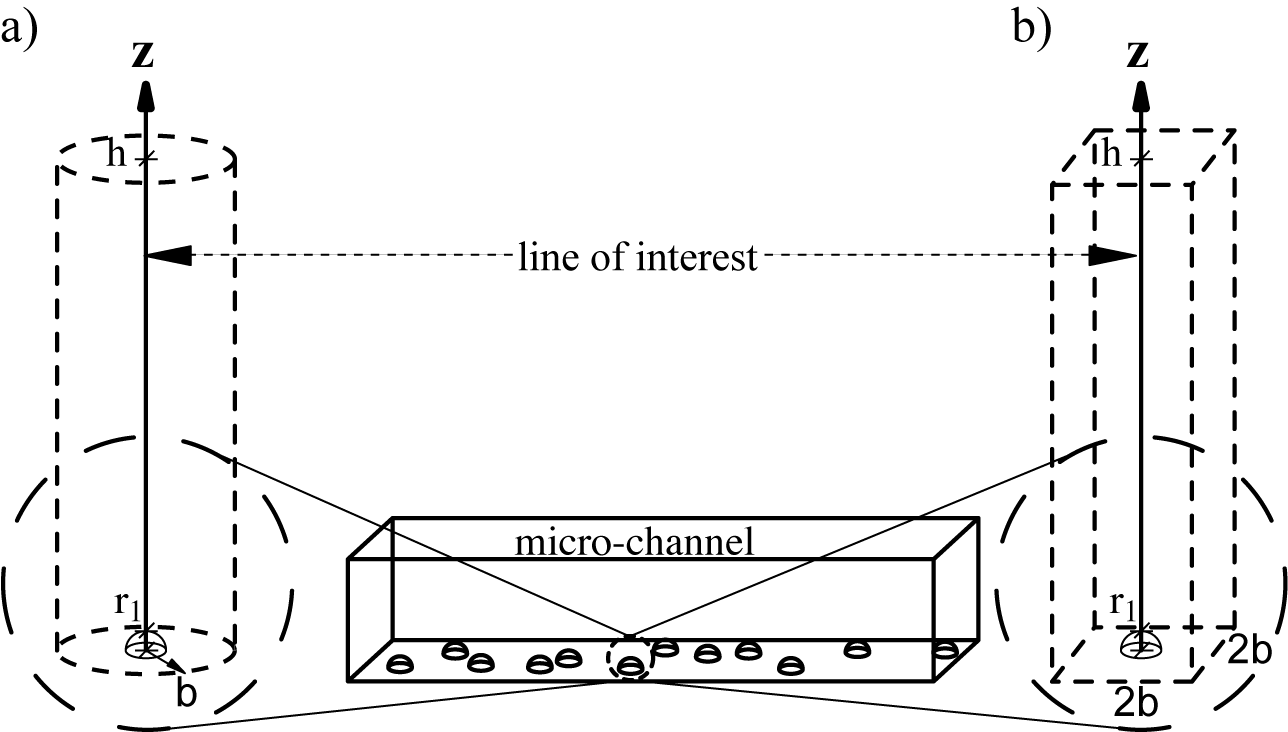
\includegraphics[width=3.5in]{Average_Geometries.pdf}
%\caption{Schematic representation of the cylindrical and rectangular geometry used to estimate the case of a single cell in culture with neighbors on a 2-D substrate. The area of the base of the unit-cylinder and unit-rectangle is equal to the area-per-cell on the substrate of the channel.}
%\label{App:Diffusion:diffusionGeom}
%\end{figure} 
%
%The line of interest labeled in Fig \ref{App:Diffusion:diffusionGeom} is the line on which a solution for the concentration will be approximated. The various ratios of the base dimension ($b$) to the height ($h$) and cell radius ($r_{1}$) will be accounted for in the boundary conditions of the one-dimensional approximation. The base dimension of the average volume is calculated from the average area per cell and the geometry. The cell is pictured as a hemisphere of radius $r_{1}$.  Items of interest emitted from or absorbed by the cell could include viruses, growth factors, cytokines, waste, or gas and have a wide range of diffusivities. The local environment of the cell has zero flux on all the walls where, on average, adjacent cells are assumed to be producing the same molecule at approximately the same rate.  An arbitrary boundary condition can be imposed at the top of the channel, $z=h$. However, we are restricted to a zero flux boundary condition at the bottom surrounding the cell, $z=0$.
%
%\section{Approximation Method}
%FE models of the average volume show that there appear to be two important regions of the model. The spherically shaped region closest to the cell and the very linear region extending far from the cell along the line of interest. These observations suggest it might be possible to add the solution of a spherical system that only depends on the radius, $r$, with a one-dimensional solution in Cartesian coordinates to obtain a total solution with sufficient accuracy to model the average cellular microenvironment (see Fig \ref{App:Diffusion:boundaries}). The idea of a linear combination to obtain the approximation is shown in Eq \ref{equ:linAdd} where $\alpha$ and $\beta$ represent the weighting of the terms in the total solution. As an addition note, other methods other than a simple linear addition were investigated, such as those that would transition between the solutions or vary the weighting with distance along the line of interest, yet they produced only slightly better results with the disadvantage of added complexity. Subscript $a$ refers to the approximation obtained from the one-dimensional solutions. Subscript $s$ refers to the one-dimensional spherical system and $c$ refers to the one-dimensional Cartesian system.
%
%\begin{figure}[!ht]
%\centering
%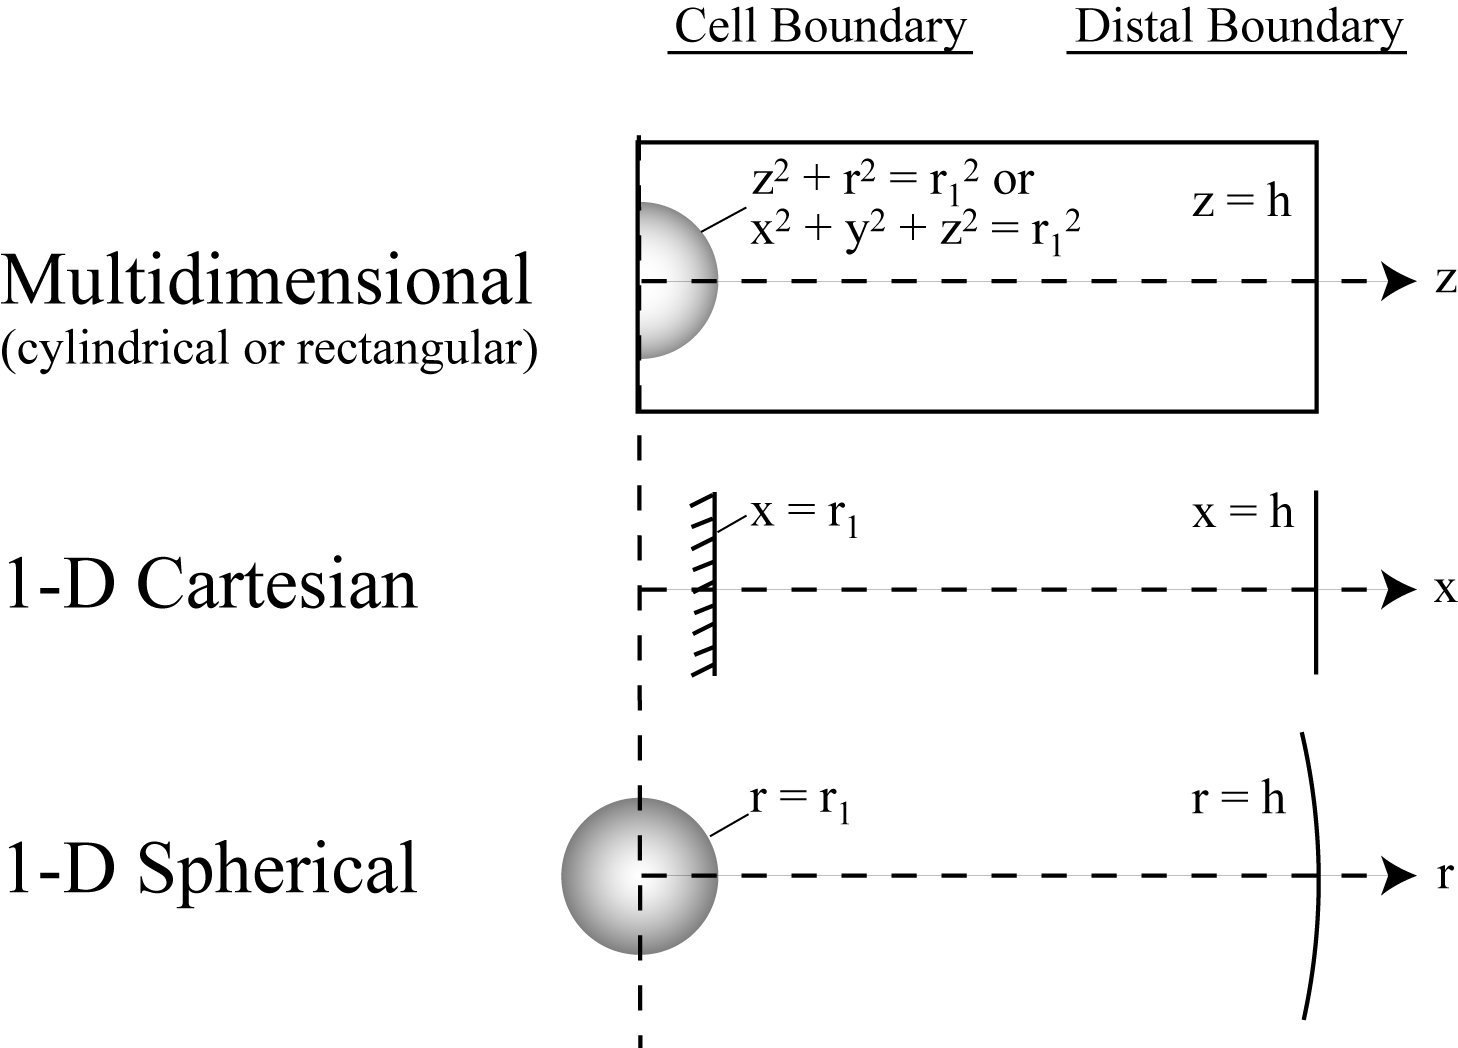
\includegraphics[width=3.5in]{Diffusion_Boundaries.pdf}
%\caption{Coordinate systems for the multidimensional models as well as the one-dimensional models.}
%\label{App:Diffusion:boundaries}
%\end{figure}
%
%
%\begin{equation}
%C_{a} = \alpha \, C_{s} + \beta \, C_{c}
%\label{equ:linAdd}
%\end{equation}
%
%Two conditions were imposed on the boundary conditions of the one-dimensional solutions to effectively determine $\alpha$ and $\beta$. The first condition was the conservation of mass. The change in average concentration with time for the volume must be the same between the multidimensional model and the approximation, as shown in Eq \ref{equ:balMass}. The second imposed condition is that the sum of the concentration gradients used in the one-dimensional system must equal the concentrations gradient perpendicular to cell boundary in the multidimensional model. The second condition is shown in Eq \ref{equ:balGrad} where $\overrightarrow{n}$ is the unit vector that points outward normal to the cell surface. Subscript $m$ refers to the multidimensional system in which all geometry is modeled precisely. 
%
%\begin{equation}
%\frac{d \overline{C}_{m}}{ d t} = \frac{ d \overline{C}_{s}}{ d t} + \frac{ d \overline{C}_{c}}{ d t}
%\label{equ:balMass}
%\end{equation}
%
%\begin{equation}
%\left( \frac{\partial C_{m}}{ \partial n} =  \frac{ \partial C_{s}}{ \partial r} + \frac{ \partial C_{c}}{ \partial x} \right) \Big |_{\textrm{\tiny cell boundary}}
%\label{equ:balGrad}
%\end{equation}
%
%By combining these conditions, the following equations for the flux boundary condition at a given time is as follows.
%
%\begin{equation}
%\label{equ:gradCart}
%\left(\frac{\partial{C_{c}}}{\partial{x}} = \frac{\partial C_{m}}{ \partial n}  \frac{ \mu-\eta}{\mu-\frac{1}{h-r_{1}}}\right) \Big |_{\textrm{\tiny cell boundary}}
%\end{equation}
%
%\begin{equation}
%\label{equ:mu}
%\mu=\frac{-3r_{1}^{2}}{h^{3}-r_{1}^{3}}
%\textrm{, and}
%\end{equation}
%
%\begin{equation}
%\label{equ:eta}
%\eta=\frac{-2\pi r_{1}^{2}}{\pi b^{2}h-\frac{2}{3}\pi r_{1}^{3}} \textrm{   (cylindrical)}
%\end{equation}
%
%\begin{equation}
%\label{equ:eta}
%\eta=\frac{-2\pi r_{1}^{2}}{4b^{2}h-\frac{2}{3}\pi r_{1}^{3}} \textrm{   (rectangular)}
%\end{equation}
%
%Eq \ref{equ:balGrad} is then used to calculate the flux boundary condition $\partial C_{s}/ \partial r$ at the cell boundary from the solution to Eq \ref{equ:gradCart}. Eq \ref{equ:gradCart} is used to create Fig \ref{App:Diffusion:ratio} where the ratio of the boundary conditions is between 0 and 1. If the ratio is $<0$ or $>1$, then the approximation method breaks down producing opposing boundary conditions. For the cylindrical geometry the ratio is 0 when $h/b= 3/ \sqrt{6}$ and where $h/b=\sqrt{6/ \pi}$ in the case of the rectangular geometry. Similarly, the ratio is 1 when $b=r_{1}\sqrt {-6h( 2r_{1}-3h}/(3h)$ and $b=r_{1}\sqrt {-6h\pi( 2r_{1}-3h)}/(6h)$ for the cylindrical and rectangular case respectively. The ratio is used to solve the one-dimensional problems over the distance $r=r_{1}\,...\,h$ with a diffusion coefficient, $D$, for the molecule of interest.
%
%\begin{figure}[!ht]
%\centering
%\includegraphics[width=2.5in]{Ratio_080207.pdf}
%\caption{Plot of $(\partial C_{c}/ \partial x)/(\partial C_{m}/ \partial n)$ for various ratios of $b/r_{1}$ and $h/r_{1}$ for the cylindrical geometry shown in Fig Xa.}
%\label{App:Diffusion:ratio}
%\end{figure}
%
%
%\section{Results and Discussion}
%\subsection{Constant flux boundary condition}
%The FE modeling software, COMSOL (PLACE), is used in conjunction with Matlab to produce all the transient diffusion results. The accuracy of the approximation is examined first using the simple case of a constant flux boundary condition on the cell. A simulation is performed for a cell with an average cell with a diameter of 10 $\mu$m producing glucose with a diffusion coefficient $D$ = 0.0016 mm$^{2}$/s at a rate of $R$ = 5.56$\times$10$^{-6}$ nmol/cell/s in a microchannel of height $h$ = 250 $\mu$m with 300 cells/mm$^{2}$. 
%%
%%\begin{figure}[!ht]
%%\centering
%%\includegraphics[width=2.5in]{box.jpg}
%%\caption{Plot of concentration vs. time for the cell boundary and ceiling of the microchannel for the multidimensional model, $C_{m}$, and the approximation, $C_{a}$, for the geometry shown in Fig Xb and parameters listed above.}
%%\label{App:Diffusion:graphCt}
%%\end{figure}
%
%Fig \ref{App:Diffusion:graphCt} shows how the approximation tracks with the 3-D COMSOL model. Notice that the difference between the approximation and multidimensional model grows until it stabilizes to a constant difference when the system stabilizes and uniformly raises in concentration over time according to Eq \ref{equ:balMass}. In order to present a comparison of the multidimensional model and approximation over a large range of geometric aspect ratios, the system is made dimensionless. Time is made dimensionless using Eq \ref{equ:tau}. Error will be reported as the percent difference between the multidimensional model and the approximation calculated at the cell boundary for $\tau$ = 1. The value of 1 is chosen for $\tau$ as it is indicative of the time it takes for a system to approach steady-state with constant flux boundary conditions. Error is plotted for various aspect ratios of the cylindrical geometry on a contour plot in Fig \ref{App:Diffusion:errorCyl}. The same is done for the rectangular geometry in Fig \ref{App:Diffusion:errorRect}.
%
%\begin{equation}
%\label{equ:tau}
%\tau = \frac{ \left( h - r_{1} \right) ^{2}}{2D}
%\end{equation}
%
%\begin{figure}[!ht]
%\centering
%\includegraphics[width=2.5in]{Cylindrical_080207.pdf}
%\caption{Error results for a constant flux boundary condition. Above is a plot of $100 \% \times (C_{m}-C_{a})/C_{m}$ for various ratios of $b/r_{1}$ and $h/r_{1}$ for the cylindrical geometry shown in Fig Xa.}
%\label{App:Diffusion:errorCyl}
%\end{figure}
%
%\begin{figure}[!ht]
%\centering
%\includegraphics[width=2.5in]{/Users/warrick/Documents/Videos_and_Images/box.jpg}
%\caption{Error results for a constant flux boundary condition. Above is a plot of $100 \% \times (C_{m}-C_{a})/C_{m}$ for various ratios of $b/r_{1}$ and $h/r_{1}$ for the rectangular geometry shown in Fig Xb.}
%\label{App:Diffusion:errorRect}
%\end{figure}
%
%Results from this section suggest that the method of approximation is valid and quite accurate for a large range of aspect ratios and cell densities. Figs \ref{App:Diffusion:errorCyl} and \ref{App:Diffusion:errorRect} indicate errors typically less than 10\% in magnitude within the applicable range of aspect ratios shown in Fig \ref{App:Diffusion:ratio}. Typical microchannel heights for cell culture are many multiples of the cell radius. If a cell is roughly 10 $\mu$m in diameter, and $h/r=30$, the microchannel height is approximately 150 $\mu$m and the approximation would be appropriate where cell density is $>57$ cells/mm$^{2}$. If $h/r=50$, then the channel height would be 250 $\mu$m and the approximation would be appropriate for cell densities $>20$ cells/mm$^{2}$. Thus, the approximation is valid for many typical cell culture parameters and can be applied as the cells proliferate and approach confluency.
%
%
%\subsection{Transient flux boundary condition}
%With positive results in the case of constant flux it is now necessary to address the situation of transient flux. The flux boundary condition is made to follow a Gaussian profile over time. A Gaussian profile is determined by the value for the mean ($\bar x$), standard deviation ($\sigma$), and maximum ($y_{max}$). The profile mean is at $\tau=1.\bar3$. $\sigma$ corresponds to $0.\bar3$ units of dimensionless time, $\tau$. Thus, at $\tau=0$ the flux is at $-4\sigma$ along the Gaussian profile. This situation might approximate the transient response of a cell to a stimulus. Typical results for the two methods using a cylindrical geometry are plotted in Fig \ref{App:Diffusion:errorTime} along with a normalized plot of the flux profile. The difference between the two methods increases during the rise in concentration and then approaches zero as the system stabalizes. The percent difference in cell boundary concentration at the peak of the flux (i.e. at $\tau=1.\bar3$) between the multidimensional model and the approximation using the cylindrical geometry is reported in Fig \ref{App:Diffusion:errorTime} for various aspect ratio as a contour plot. Results show good agreement with the multidimensional model again with similar errors as the case of a constant flux boundary condition.
%
%\begin{figure}[!ht]
%\centering
%\includegraphics[width=2.5in]{Cylindrical_Transient_080207.pdf}
%\caption{Error results for a transient flux boundary condition following a Gaussian profile. Above is a plot of $100 \% \times (C_{m}-C_{a})/C_{m}$ for various ratios of $b/r_{1}$ and $h/r_{1}$ for the cylindrical geometry shown in Fig Xa.}
%\label{App:Diffusion:errorTime}
%\end{figure}
%
%
%
%
%
%
%
%
%\subsection{Dynamics of diffusion and biology}
%One typical change during \textit{in-vitro} cell culture is the cell number. A major advantage of reducing the multidimensional diffusion problem to a one-dimensional problem is that changes in cell number (i.e. the spacing parameter $b$) can be accounted for using Eq \ref{equ:gradCart}. Thus, the approximation method can accommodate changes in cell density due to cell proliferation, death, or apoptosis by adjusting the flux boundary condition accordingly. There is no need to interrupt the model and incrementally re-mesh the geometry making the FE model impractical for many users. 
%
%Through simulation one can also identify when diffusion dynamics result in significant concentration differences within the system and could possibly affect cell behavior. One way to estimate the concentration distribution within the channel is to look at a steady-state system with constant flux at the cell. At steady-state, the difference, $\triangle C$, between the concentration at the cell boundary and at the ceiling of the channel for the approximation are given by the following equations.
%
%\begin{equation}
%\label{equ:steady}
%\triangle C=\frac{\alpha}{r_{1}-h}+\frac{\beta}{2}(r_{1}^{2}-h^{2}) + \frac{h-r_{1}}{2} \left(\frac{\partial C_{c}}{\partial x} \big |_{x=r_{1}}\right)
%\end{equation}
%
%\begin{equation}
%\label{equ:alpha_2}
%\alpha = -\beta r_{1}^{3}+ r_{1}^{2} \left(\frac{\partial C_{s}}{\partial r} \big |_{r=r_{1}}\right)
%\end{equation}
%
%\begin{equation}
%\label{equ:beta_2}
%\beta = -\frac{r_{1}^{2}}{h^{3}-r_{1}^{3}} \left(\frac{\partial C_{s}}{\partial r} \big |_{r=r_{1}}\right)
%\end{equation}
%
%$\triangle C$ is affected by the dimensions of the system and the rates of influx and efflux to and from the cell. Concentration differences increase with increasing dimensions and increasing rates of flux. $\triangle C$ can be compared to other important concentration parameters of the system. For example, if the initial concentration of nutrients within a microchannel, $C_{0}$ is $\gg \triangle C$ then the dynamics of diffusion will have little relative effect on concentrations. However, if $C_{0} \sim \triangle C$ or if nutrients are depleted to a point where the average concentration, $\overline{C}$, is on the order of $\triangle C$, then the dynamics of diffusion could play an important role in system behavior. Another consideration is the relative size of $\triangle C$ to threshold concentrations of the cell, $C_{t\_i}$. If $\triangle C \ll C_{t\_i}$, then diffusion dynamics will play little role in affecting concentrations near thresholds.
%
%The time scale and biological dynamics of the system can also be important when considering the role of diffusional effects. For example, if the time scale of the biological process is on the order of $\tau$, an estimate of the time it takes for diffusion to redistribute the soluble factor (see Eq \ref{equ:tau}), the dynamics of the biological process and diffusion will interact for unique system behavior. Alternatively, even if $\triangle C$ is relatively small and $\tau$ is much less that the time scale of the biological process, effects of the concentration distribution could be significant when integrated over a large time. For example, if a soluble factor played a critical role in exponential cell growth, over time, the effects of a small difference in concentration could be greatly magnified over time. Similarly, biological processes with tight thresholds or feedback loops could be very sensitive to subtle changes in microenvironmental concentrations due to diffusional dynamics.
%
%Some of the considerations that were just discussed can be seen in a simple model of cell growth in response to a rate limiting factor. Factor concentration and cell proliferation are dynamically modeled together using Matlab and a Crank-Nicolson method for modeling diffusion.
%
%Proliferation rate is assumed to follow the Michaelis-Menten kinetics with respect to the concentration of a rate limiting factor (Eq \ref{equ:prolRate}). $u_{max}$ represents the maximum proliferation rate of the cells. $C$ is the concentration of factor at the cell boundary and $K_{m}$ is the Monod or Michaelis-Menten constant, which is the concentration at which the proliferation is at $u_{max}/2$. Population kinetics are then modeled using Eq \ref{equ:pop} where N is the cell number. Many other terms could be included into Eq \ref{equ:prolRate} to more accurately model the system such as the possible negative effects of waste concentration or cell contact inhibition. As more soluble factors are added to the system, a separate, simultaneous model of diffusion is needed to keep track of each concentration. In the interest of simplicity, extra terms are neglected in this example. The result of the simulation (the dynamic model) will be compared to a model that assumes even and constant mixing of the microchannel (the evenly-mixed model). The hypothesis is that the distribution of soluble factors can play a significant role in the dynamics of the system as a whole.
%
%\begin{equation}
%\label{equ:prolRate}
%u = \frac{u_{max}C} {K_{m}+C}
%\end{equation}
%
%\begin{equation}
%\label{equ:pop}
%u = \frac{1}{N} \frac{dN}{dt}
%\end{equation}
%
%The cell number over time is plotted for the dynamic and evenly-mixed model are plotted over time to show the difference in the results. Tab X shows simulation results for a wide variety of parameters. In some cases, there is enough factor to double the population size while in other cases, the  factor is depleted and growth rate approaches $0$. If the population doubles, the time at which it doubles is reported as $t_{2N_{0}}$. If the population growth rate falls to one tenth of the maximum growth rate, the cell number and time, $t_{u_{max}/10}$, at which it occurs are recorded. The ratio  $(\partial C_{c}/ \partial x)/(\partial C_{m}/ \partial n$) is always between 0 and 1 in the simulations. Also $b/r$ is always $>1$. Corresponding values of $\triangle C$ and $\tau$ are given for later analysis and discussion. The time scale of the biological process is estimated here as the doubling time of the cell population when the proliferation rate is at a maximum and is referred to using $t_{bp}$.
% \chapter{Concentrator: Additional Information}
\label{App:Concentrator}

\section{Estimation of Cell Number Limit}

A lower limit of ~50,000 cells is calculated based on a seeding density of 250 cells/mm$^{2}$ for culture in a microchannel with a height of 250 \textmu m (\ie , a density of 1000 cells/\textmu L). It is also assumed that the original sample is centrifuged to a minimum volume of 50 \textmu L to avoid aspiration of any concentrated cells. The limit is specific to the application.

\section{Initial Design Approach for Concentrator Design}

The dimensions of the initial device design were chosen in order to produce a shear stress of roughly 0.1 dynes/cm$^{2}$ within the collection region and to give the cells a chance to settle to the substrate after entry into the collection region (i.e., t$_{set}/t_{res}$ $\approx$ 1). Transport channel dimensions were then varied to produce shear rates and residence times above and below these thresholds to explore the appropriate conditions for proper cell retention. Channel resistances were estimated using the Washburn Law and applied to an electrical circuit analog for fluid flow. Passive pumping pressures were estimated using Eq \ref{equ:laplace}.

Design II differs from Design I primarily in the dimensions of the collection region. The width was increased while the height was reduced based on the dimensional analysis described in the main text. Channel height does not affect t$_{set}/t_{res}$ but can affect shear. When channel width increases, t$_{set}/t_{res}$ decreases, thereby increasing the chance for cell capture. Thus Design II was viewed as an improvement to Design I.

\section{Cell Loss Modeling}

COMSOL Multiphyisics v3.4 (Burlington, MA) was used to obtain steady state solutions for fluid flow through Deisgn I and II. First a simulation of the whole device (using symmetry) was used to determine that the pressure drops across the transport channels (from center input to the outer ring) were within 0.55\% of one another (see Fig \ref{fig:evenPressure}). Because flow through each transport is nearly identical, the 3D model was simplified to include only one of the repeating sections of the collection region. This repeating section was then divided in half along its line of symmetry. This allowed a finer meshing of the region for more detailed analysis.

\begin{figure}[!b]
\centering
\includegraphics[width=3in]{EvenPressure_Composite.pdf}
\caption{\textbf{Plot of normalized pressure along device axis of symmetry}. The pressure at the input is defined as 1 whereas the pressure nearest the output port is defined as zero. The normalized pressure farthest from the output, at the intersection of the transport channel and outer ring, is then 0.0055.}
\label{fig:evenPressure}
\end{figure}

A threshold of 0.1 dynes/cm$^{2}$ was used to help determine cell loss (see Fig \ref{fig:shearStress}). If streamline calculations suggest that a cell settles to the surface before reaching the collection region exit, then the shear stress is calculated at that location. If the shear stress at that location is below the threshold of 0.1 dynes/cm$^{2}$, then the cells that follow that streamline are assumed to be captured. If the shear stress is too high, it is assumed the cells are lost. Only one half of the region depicted was simulated using a symmetry boundary condition along the center line. The results are reflected to better indicate the shape of the repeating portion of the collection region.

\begin{figure}[!b]
\centering
\includegraphics[width=3in]{ShearStress.pdf}
\caption{\textbf{Concentrator shear stress near the substrate}. Shear stress one cell radius (6.25 \textmu m) above the substrate for a total device flow rate of 5 \textmu L/min. The color legend indicates shear stresses between 0 and 0.1 dynes/cm$^{2}$. Simulations assume that cells are not collected in regions with a shear stress above 0.1 dynes/cm$^{2}$ (white areas near inlet and outlet). Flow velocities in the x-direction half way through the collection region are shown as a slice heat map.}
\label{fig:shearStress}
\end{figure}

Streamlines were modeled by assuming that the cell settles at a rate of 2.7 \textmu m/s, a value obtained using the Stokes drag of the particle. Streamlines were calculated using COMSOL starting at the entrance into the collection region (see Fig \ref{fig:streamlines}). The starting points form a grid in the entrance. The size of the cell prohibits the center of the cells from following streamlines that are less than a radius from the transport channel wall. Thus the grid of streamline start-points begin one radius in from the transport channel walls. The streamlines are followed until the ``cell'' exits the modeled space (\ie , the substrate or collection region exit).

\begin{figure}[!t]
\centering
\includegraphics[width=3in]{StreamlinePlot.pdf}
\caption{\textbf{Particle streamlines within the concentrator}. Example plot of streamlines used to calculate percent loss for a given flow condition and device design. Streamlines begin from a grid of locations at the entrance to the collection region. The streamlines are followed until they exit the collection region or intersect with the substrate of the device. These streamlines are calculated assuming the cell settles at a velocity of 2.7 \textmu m/s and used in further calculations to determine if the cell is captured or lost. A high density of streamlines is used to increase the precision of the simulated loss measurements.}
\label{fig:streamlines}
\end{figure}

By numerically integrating the inverse of the particle velocity along the length of a streamline, one can obtain the time it takes for the particle to reach a location along that streamline. The amount of fluid that has flowed along the streamline is equal to the flow rate at the starting point times the time that has been allowed to pass. The flow rate at the starting point of the streamline is dictated by the fluid velocity and the grid spacing for the streamlines. The information regarding the time for the particles to reach a location along the streamline can be converted to volume information using this flow rate. In other words, the data is transformed such that it represents how much volume must flow into the device to move the particles to a certain position along a streamline. The volume-position data for each streamline is then used to determine how many cells would be lost for a given streamline, cell suspension density, and volume that has been pumped at a predetermined average flow rate. This method simplifies pumping as a square wave instead of a natural passive pumping flow profile. The average flow rate used to calculate cell loss is determined by taking the volume-averaged flow rate of a passive pumping profile that matches the given experimental condition. The method described here does take into account fixed-volume effects as described in the main article. If not enough fluid has been put through the device to cause any cells to leave the collection region on a streamline, all the cells on that streamline are considered captured.

\section{Experimental Calculation of \texorpdfstring{{\boldmath$t_{set}/t_{res}$}}{tset tres}}

Passive pumping is a dynamic phenomena where pressure changes with the geometry of the droplet that drives fluid flow. In order to estimate a value for $Q$ from this dynamic process for use in Eq \ref{equ:ratio}, an `average' value must be chosen.  A volume-averaged flow rate is chosen instead of a time-averaged flow rate as we are interested in the average velocity that a particular unit volume sees within the collection region. The volume-averaged flow rate can be calculated from the volume-averaged pressure, $P$, and resistance, $Z$, given that $P=QZ$ for low Reynolds number flow. The volume-averaged pressure can be determined using the relationship between droplet geometry and pressure given by the Young-Laplace equation (Eq \ref{equ:laplace}). The resistance of the device was determined using experimental measurements of passive pumping times and droplet geometries, as measured using a goniometer. The data was matched with an analytical solution for passive pumping\cite{Berthier:2007mi} to determine the device resistance, $Z$, needed to produce the appropriate pumping time given the initial droplet geometry. This resistance, volume-averaged pressure, and device geometry ($A$) are then used to calculate an appropriate flow velocity, $v_{f}$, for estimating $t_{set}/t_{res}$. The cross sectional area, A, is calculated at the average radius of the device collection region, $r_{d}$ = 3.75 mm. 

Calculations of flow rate in Design II are summarized in Fig \ref{fig:pp}. Instead of plotting pressure \vs\ volume, device geometry and resistance are taken into account to plot flow rate \vs\ volume. Results for a 6 \textmu L and 15 \textmu L drop are shown as these are the two different sizes of drops used experimentally. Simulated cell trajectories are depicted in a cross-section view of the collection region and show how higher flow rates cause more cell streamlines to flow out of the collection region instead of reaching the substrate. The trajectories are simulated using steady-state conditions and are only shown for those along the centerline of the transport channels.

% \chapter{Oscillatory Flow}
\label{App:Oscillator}

Below is a table with the constants and variables used throughout this appendix with their definitions.

\begin{table}[!ht]
\caption{\textbf{Variables and constants of fluid flow and their definitions}.}
\centering
\begin{tabular}{cp{10.5cm}}\toprule
Variable/Constant & Description \cr \midrule
$p$ & pressure \cr
$\delta$ & constant pressure gradient amplitude \cr
$\delta_{o}$ & oscillating pressure gradient amplitude \cr
$\rho$ & fluid density \cr
$\mu$ & dynamic viscosity of the newtonian fluid \cr 
$\nu$ & kinematic viscosity, $=\mu/\rho$ \cr
$f$ & frequency of the oscillatory pressure gradient \cr
$\omega$ & radial frequency, $=2\pi f$ \cr 
$h$ & the full height of the channel \cr
$\lambda$ & penetration depth, $=\sqrt{2\nu/\omega}$ \cr 
$u$ & fluid velocity \cr
$\bar u$ & average fluid velocity \cr
$u_{max}$ & maximum fluid velocity \cr
$\tau_{wall}$ & fluid shear stress at the top and bottom surface of the channel \cr
$\tau_{wall, o}$ & fluid shear stress at the top and bottom surface of the channel due to the oscillatory component of flow\cr
$\gamma_{wall}$ & fluid shear rate at the top and bottom surface of the channel \cr
\bottomrule
\end{tabular}
\label{tab:}
\end{table}

We first present the solution to steady laminar flow between parallel plates as it will be references later in the context of oscillatory flow.

\section{Steady Laminar Flow Between Parallel Plates}
With the origin positioned half way between the plates (\ie , $y=0$) and the full height of the channel defined as $h$, the equation for $u$, the velocity in the x-direction is as follows.

\begin{equation}
\centering
u= \frac{1}{2\mu}\left[\frac{d}{dx}(p+\rho g z)\right]\left(\left(y-\frac{h}{2}\right)^{2}-\frac{h^{2}}{4}\right)
\label{equ:u}
\end{equation}
The flow rate through the cross section, where $b$ is the width that is $\gg h$ is as follows.
\begin{equation}
\centering
Q=-\frac{bh^{3}}{12\mu}\left[\frac{d}{dx}(p+\rho g z)\right]
\label{equ:Q}
\end{equation}
The average velocity of fluid between the plates is
\begin{equation}
\centering
\bar u = -\frac{h^{2}}{12\mu}\left[\frac{d}{dx}(p+\rho g z)\right] = \frac{Q}{bh} = \frac{2}{3}u_{max}.
\label{equ:ubar}
\end{equation}
The wall shear stress is given by the following.
\begin{equation}
\centering
\tau_{wall} = -\frac{h}{2} \left[\frac{d}{dx}(p+\rho g z)\right] = \frac{6\mu Q}{bh^{2}} = 2\mu \gamma_{wall}
\label{equ:tauWall}
\end{equation}

\section{Oscillatory, Non-Turbulent Flow Between Parallel Plates}

The mathematical analysis of oscillatory flow in a microchannel that can be approximated as a parallel plate flow chamber is presented here along with analysis of how much the surface tension at the ports of a tubeless microchannel influences flow. The following closed form solutions for oscillatory flow are reproduced from Bacabac \etal, 2005 \cite{Bacabac:2005ax} who compiled the information from Landau \etal, 1959 \cite{Landau:1959vh}. 

The equation for the velocity $u$ at vertical position $y$ in the channel at time $t$ where $y=0$ is half-way between the plates and h is the distance between the plates is given by Eq \ref{equ:uofyt} with subelements given by the equations that follow.

\begin{equation}
u(y,t)=C_{1}(y)+C_{2}(y)cos(\omega t)+C_{3}(y)sin(\omega t)
\label{equ:uofyt}
\end{equation}

\begin{equation}
C_{1}(y)=-\frac{\delta}{2\mu}\left(y^{2}-\frac{h^{2}}{4}\right)
\label{equ:C1}
\end{equation}

\begin{equation}
C_{2}(y)=\frac{\delta_{0}}{\rho\omega}\left[\frac{CC\left(\frac{-y+\frac{h}{2}}{\lambda},\frac{y+\frac{h}{2}}{\lambda}\right)+CC\left(\frac{y+\frac{h}{2}}{\lambda},\frac{-y+\frac{h}{2}}{\lambda}\right)}{cc_{+}\left(\frac{h}{\lambda}\right)}-1\right]
\label{equ:C2}
\end{equation}

\begin{equation}
\footnote{I believe that there is a typo in this equation of Bacabac \etal . The discrepancy is in the signs of the arguments of the second SS function. Otherwise, the results do not match the results in the paper or those obtained using COMSOL simulation as a secondary check.}C_{3}(y)=\frac{\delta_{0}}{\rho\omega}\left[\frac{SS\left(\frac{-y+\frac{h}{2}}{\lambda},\frac{y+\frac{h}{2}}{\lambda}\right)+SS\left(\frac{y+\frac{h}{2}}{\lambda},\frac{-y+\frac{h}{2}}{\lambda}\right)}{cc_{+}\left(\frac{h}{\lambda}\right)}\right] 
\label{equ:C3}
\end{equation}

\begin{equation}
\lambda = \sqrt{\frac{2\nu}{\omega}}
\label{equ:lambda}
\end{equation}


\begin{equation}
\begin{array}{r@{=}l}
SS(x_{1},x_{2})&\sin(x_{1})\sinh(x_{2}) \cr
CC(x_{1},x_{2})&\cos(x_{1})\cosh(x_{2}) \cr
ss_{\pm}(x)&\sin(x)\pm\sinh(x) \cr
cc_{\pm}(x)&\cos(x)\pm\cosh(x) \cr
\end{array}
\label{equ:C4}
\end{equation}

From these solutions, Bacabac \etal\ defined correction factors for the amplitude of the fluid flow rate and wall shear stress amplitude by normalizing results by the value predicted for static flow. Thus, when the correction factors are significantly different than 1, static solutions to the flow are no longer good approximations and dynamic effects are becoming significant. $T$ is the wall shear stress correction factor (when the flow rate is known) while $K$ is the correction factor for the amplitude of the flow rate, $q$ when the pressure gradient is known. Thus, if one is predicting shear when the pressure gradient is known, one must correct the flow rate using $K$ and plug the adjusted flow rate into the equation for shear which is then adjusted by $T$.

I was unable to successfully reproduce results given the Bacabac version of the equation for $K$ but was able to implement $T$ and the product $TK$, from which $K$ can be obtained through division. The following equations are used to predict flow and wall shear stress due to the oscillatory component of flow.

\begin{equation}
T(h/\lambda) = \frac{1}{3\sqrt{2}}  \frac{\frac{h}{\lambda}}{cc_{+}(\frac{h}{\lambda})}   \sqrt{\frac{(\sin(h/\lambda))^{2}+(\sinh(h/\lambda))^{2}}{1-\frac{2(\frac{\lambda}{h})ss_{+}(h/\lambda)}{cc_{+}(h/\lambda)}-\frac{2(\frac{\lambda}{h})^{2}cc_{-}(h/\lambda)}{cc_{+}(h/\lambda)}}}
\label{equ:T}
\end{equation}

\begin{equation}
T(h/\lambda)K(h/\lambda) = \frac{\sqrt{\left(ss_{-}(h/\lambda)\right)^{2}+\left(ss_{+}(h/\lambda)\right)^{2}}}{\frac{h}{\lambda}\;cc_{+}(h/\lambda)}
\label{equ:TK}
\end{equation}

\begin{equation}
q_{o}=\frac{bh^{3}\gamma_{o}}{12\mu}K(h/\lambda)
\label{equ:q}
\end{equation}

\begin{equation}
\tau_{wall, o}=\frac{6\mu q_{o}}{bh^{2}}T(h/\lambda)=\frac{h\gamma_{o}}{2}T(h/\lambda)K(h/\lambda)
\label{equ:tau}
\end{equation}

Bacabac \etal\ point out in their paper that $T$ does not vary significantly for $h/\lambda<2$ while $K$ does not vary significantly for $h/\lambda<1$. The thresholds are different because inertial effects on flow rate can be felt before the parabolic flow profile is significantly altered, at which point the shear stress for a given flow rate is altered. Therefore, the threshold of $h/\lambda<2$ is to be used as a predictor of quasi-parabolic flow whereas the threshold of  $h/\lambda<1$ should be used to determine when steady flow can be assumed to provide accurate predictions for a given instant in time.

Using the threshold of $h/\lambda<2$, one can predict the critical frequency, $f_{c}$, of a system using Eq \ref{equ:fcrit};

\begin{equation}
f_{c} = \frac{4\mu}{\rho\pi h^{2}}
\label{equ:fcrit}
\end{equation}

It should also be noted that Bacabac also cites Loudon \etal\ who empirically related the Womersley number (a number that characterized the balance of viscous and inertial forces in oscillatory flow) and the Reynolds number, $Re$ \cite{Loudon:1998sf}. Loudon \etal\ found that the Reynolds number was approximately 150-250 times the Womersley number in the blood vessels of dogs. Using this relation and assuming that the transition to turbulence occurs near $Re=2000$, we can predict that turbulence in the parallel plate flow chamber would occur at around $h/\lambda=8/\sqrt{2}\approx5.7$. Thus, we can also characterize the turbulence of the system using the same dimensionless quantity $h/\lambda$.


%(1/(sqrt(2)*3)) * (r/fun('cc+',r,0)) * (sqrt(((sin(r))^2+(sinh(r))^2)/(1-(2*(1/r)*fun('ss+',r,0))/(fun('cc+',r,0))-(2*(1/r)^2*fun('cc-',r,0))/(fun('cc+',r,0)))))

\section{Steady Flow in a Rectangular Duct}

A relatively simple expression that agrees with resistance in rectangular ducts is given by the Washburn law, taken from and reproduced here in Eq \ref{equ:Washburn} from \cite{Shah:1978fb}. Eq \ref{equ:Washburn} simplifies to the case of flow between parallel plates when the aspect ratio ($\lambda=$width/height$ = w/h$) of the rectangular duct is $>4.45$. The variable L is the length of the duct and $\mu$ is the dynamic viscosity of the fluid.

\begin{equation}
\centering
K=\frac{8\,\mu\,L\,g(\lambda)}{h^{3}\,w}
\label{equ:Washburn}
\end{equation}

\begin{displaymath}
\centering
g=\left\{\begin{array}{cl}\frac{3}{2}&\textrm{if }\lambda>4.45\cr\frac{(1+\lambda)^{2}}{\lambda^{2}}&\textrm{if }\lambda<4.45\cr\end{array}\right.
\end{displaymath}

The following correction factor for shear stress in a rectangular duct is taken from \cite{NATARAJA.NM:1973fk}.
\begin{equation}
\centering
\tau_{w}= \frac{6 \mu Q}{wh^{2}}\frac{m+1}{m} \textrm{, for $h/w < 0.33$}
\end{equation}

\begin{equation}
\centering
m = 1.7 + 0.5 \left(\frac{h}{w}\right)^{-1.4}
\end{equation}

\section{Shear Stress from Amplitude}

You don't need to use a correction factor to find shear stress for the center portion of a rectangular duct if you measure amplitude of a particle in motion. This is because in the center portion, the amplitude of the particle gives an accurate indication of the maximum velocity for the nearly parabolic flow in that region. If you measure the amplitude, $A$, where particle position is $Asin(2\pi ft)$ and know the frequency, $f$, you can use Eq \ref{equ:amp} to get the shear stress, $\tau_{w}$.

\begin{equation}
\centering
x=A \sin (2\pi f t)
\label{equ:amp}
\end{equation}

\begin{equation}
\centering
\frac{dx}{dt} = u = 2 \pi A f \cos (2\pi f t)
\label{equ:dxdt}
\end{equation}

\begin{equation}
\centering
u_{max} = 2 \pi A f
\label{equ:umax}
\end{equation}

Given,

\begin{equation}
\centering
\bar u = \frac{Q}{bh} = \frac{2}{3}u_{max}
\label{equ:ubar2}
\end{equation}

and

\begin{equation}
\centering
\tau_{wall} = \frac{6\mu Q}{bh^{2}}
\label{equ:tauWall2}
\end{equation}


then,

\begin{equation}
\centering
\tau_{wall} = \frac{Q}{bh}\frac{6\mu}{h} = \frac{2}{3}u_{max}\frac{6\mu}{h} = \frac{2}{3}2 \pi A f \frac{6\mu}{h} = \frac{8 \pi A f \mu}{h}
\label{equ:tauWall3}
\end{equation}

\begin{equation}
\centering
\tau_{w}= \frac{8 \pi A f \mu}{h}
\label{equ:tauWall4}
\end{equation}

In order to find the amplitude desired for a given geometry and shear stress, the equation is rearranged as follows.

\begin{equation}
\centering
A = \frac{h \tau_{w}}{8 \pi f \mu}
\end{equation}

For a channel height of 140 $\times$ $10^{-6}$ [m] and a viscosity of 0.00078 [kg/ms] the equation simplifies to the following.

\begin{equation}
\centering
A = 0.00714 \frac{\tau_{w}}{f} \textrm{ [Pa]}
\end{equation}

\section{Units and Conversions}

Water is 1 cP or 0.01 P.
\begin{equation}
\centering
1 \textrm{ Poise} = 1 \textrm{ g/cm\,s} = 0.1\textrm{ kg/m\,s}
\end{equation}

\begin{equation}
\centering
1 \textrm{ Pascal or kg\,m/s}^{2} = 10 \;\mathrm{ dynes/cm}^{2} \textrm{ or g/cm\,s}^{2}
\end{equation}

\begin{equation}
\centering
1 \;\mathrm{ Newton} = 100\,000 \;\mathrm{ dynes}
\end{equation}

\begin{equation}
\centering
1 \;\mathrm{ kg/m\,s} = 10 \textrm{ P or g/cm\,s}
\end{equation}

Therefore multiply $\partial v_{x}/\partial y$ of units [1/s] by $\mu$, 0.00078 [kg/ms] for DMEM with supplements, to get shear stress in Pa and then multiply the shear stress that is in [Pa] by 10 to get [dynes/cm$^{2}$].

\section{Matlab Code}

\begin{matlab}
\caption{Matlab code that defines the $C_{1}$, $C_{2}$, and $C_{3}$ of Eq \ref{equ:u}.}
\lstinputlisting{/Users/warrick/Documents/MMB_Lab/Papers_and_Chapters/Thesis_Materials/Prelim/appOscillatoryFlow/Materials/C.m}
\end{matlab}

\begin{matlab}
\caption{Matlab code that defines the functions of Eq \ref{equ:C4}.}
\lstinputlisting{/Users/warrick/Documents/MMB_Lab/Papers_and_Chapters/Thesis_Materials/Prelim/appOscillatoryFlow/Materials/fun.m}
\end{matlab}

\begin{matlab}
\caption{Matlab code that defines the shear corrections factor $T$ of Eq \ref{equ:T}.}
\lstinputlisting{/Users/warrick/Documents/MMB_Lab/Papers_and_Chapters/Thesis_Materials/Prelim/appOscillatoryFlow/Materials/T.m}
\end{matlab}

\begin{matlab}
\caption{Matlab code that defines the product of the shear and flow correction factors $T$ and $K$. The product is shown in Eq \ref{equ:TK}.}
\lstinputlisting{/Users/warrick/Documents/MMB_Lab/Papers_and_Chapters/Thesis_Materials/Prelim/appOscillatoryFlow/Materials/C.m}
\end{matlab}


%Oscillatory flow can be created in an tubeless microchannel via shaking. Shaking a microchannel induces an acceleration of the microchannel and thus a pressure gradient within the channel. Due to the typically viscous dominated character of fluid flow in microchannels, the flow is typically laminar and parabolic; however, frequencies and amplitudes of oscillation can be such that the fluid flow is dominated by inertia. Further, there is another category of oscillatory flow in a tubeless channel, which is dominated by surface tension considerations. The particulars of surface tension based pressures and droplet geometry are contained in App \ref{appSurfaceTension}. Equations of flow in a microchannel that is viscous dominated are contained here and are reproduced from Bacabac \etal, 2005 \cite{Bacabac:2005ax}.

%We hope to analyze the importance of surface tension when considering a microchannel that is oscillated. For this we will consider simple oscillatory flow in a rigid tube. First, we will model the system for low frequencies (i.e. the system is dominated by viscous forces and there is a 180$^{\circ}$ phase shift between pressure gradient and and parabolic fluid flow). This situation can be described with the following equations.
%\begin{equation}
%Q = \left(-\frac{\partial P}{\partial x}\right)\frac{\pi R^{4}}{8 \mu}
%\end{equation}
%\begin{equation}
%V_{max} = \left(\frac{\partial P}{\partial x}\right)\frac{R^{2}}{4 \mu}
%\end{equation}
%\begin{equation}
%V = V_{max}\left(1-\left(\frac{r}{R}\right)^{2}\right)
%\end{equation}
%\begin{equation}
%\tau =\left( -\frac{\partial P}{\partial x}_{max}\right)\frac{R}{2}
%\end{equation}

%For small oscillations in volume, the pressure gradient from surface tension can be approximated with a 'spring constant' that relates pressure to volumetric displacement. The maximum possible value of the spring constant, $\partial P/\partial V$, is shown in Eq \ref{equ:k}. 
%\begin{equation}
%\frac{\partial P}{\partial V} = \frac{8 \gamma}{\pi a^{3}}
%\label{equ:k}
%\end{equation}
%Because the inertial lag or phase shift in the system is negligible, the flow is an instantaneous indication of the pressure gradient. Thus, the total pressure gradient on the system is the linear addition of the pressure gradient arising from oscillation of the channel and the surface tension. These effects are $90^{\circ}$ out of phase and will be represented using sine and cosine functions. Eq \ref{equ:DeltaP} comes from the second derivative of a sinusoidal input to give acceleration. The acceleration is substituted into the equation for fluid pressure due to an acceleration field, $\Delta P = \rho \ddot{x} L$. 
%\begin{equation}
%\frac{\partial P}{\partial x} = -\frac{\Delta P_{osc}}{L}\sin(\omega t)  - \frac{Vol_{max}}{L} \frac{\partial P}{\partial V}\cos(\omega t)
%\label{equ:dPdx}
%\end{equation}
%\begin{equation}
%\Delta P_{osc} = A \omega^2 \rho L
%\label{equ:DeltaP}
%\end{equation}
%\begin{equation}
%Vol_{max} = \left| \int_{\omega t = \frac{\pi}{2}}^{\omega t = \pi} \left(-\frac{\partial P}{\partial x}\right)\frac{\pi R^{4}}{8 \mu} \partial t \right|
%\end{equation}

%The result is a circular definition for $\partial P/\partial x$. However, we can gain insight by calculating terms in succession. First we calculate the solution with only the first term in Eq \ref{equ:dPdx} (i.e. with no surface tension effects) to estimate a worst case displacement for $Vol_{max}$. It is a worst case because surface tension will generally work to reduce the displacment. We then substitute the result back into Eq \ref{equ:dPdx} to get Eq \ref{equ:dPdx_wc}, a worst case scenario for $\partial P/\partial x$. Notice that resonant frequencies are not of concern here in this viscous dominated system.
%\begin{displaymath}
%Vol_{max, wc} = \left| \int_{\omega t = \frac{\pi}{2}}^{\omega t = \pi} \left(\frac{\Delta P_{osc}}{L}\sin(\omega t)\right)\frac{\pi R^{4}}{8 \mu} \partial t \right|
%\end{displaymath}
%\begin{equation}
%Vol_{max, wc} = \frac{A \omega \rho\pi R^{4}}{8 \mu}
%\end{equation}
%\begin{equation}
%\frac{\partial P}{\partial x} \approx_{wc} \left(-A \omega^{2} \rho \right) \left(\sin(\omega t)  + \frac{R^{4} \gamma}{\omega a^{3} \mu L} \cos(\omega t) \right)
%\label{equ:dPdx_wc}
%\end{equation}

%So, we can see that if the coefficient of the cosine term (i.e. the ratio of the pressure gradients from oscillation and surface tension) is much less than 1, surface tension can be ignored in the solution of the system. To see this, let $A=500 \mu$m, $\omega = 20(2 \pi)$, $L=5$mm, and $a = R = 250 \mu$m. $\Delta P_{sin}/L$ has a magnitude of 7900 Pa/m. This results in $Vol_{max} = 1.54 \times 10^{-13}$ m$^{3}$ which, when multiplied by $\partial P/\partial V$ and divided by $L$, gives 229 Pa/m for the worst case pressure gradient due to surface tension. The coefficient of the cosine term is $\approx 0.029$. The flow rates of the solution with and without the cosine term is plotted in Fig \ref{fig:LoFreq}. Thus, the pressure gradient from surface tension and can be ignored. 

%\begin{figure}[!ht]
%\centering
%\includegraphics[width=2.5in]{OscPlot.pdf}
%\caption{Low frequency approximation to oscillatory flow in a microchannel. The solid line shows the system without surface tension perturbation while it is present in the red-dashed system.}
%\label{fig:LoFreq}
%\end{figure}

%It can be seen that very low frequencies are needed to make surface tension significant, especially for reasonably size ports. Ports are generally near the same radius as the channel. For the particular case shown in Fig \ref{fig:LoFreq}, the frequency would have to be reduce by a factor of 4 from a frequency of 20 Hz to 5 Hz. 

%The range of shear stresses that we are interested in is near 0.5 dynes/cm$^{2}$ per literature on sorting of cells in continuous shear flow. Preliminary vibration results with cells showed that frequencies somewhere in the range of 5-40 Hz are necessary to affect cell adhesion. However, at a frequency of 5 Hz, the estimated shear stress is 0.6 dynes/cm$^{2}$. Therefore, this might indicate that slightly higher shear is needed when using oscillation. This is quite speculative as the initial experimental setup was very undefined. The new setup has a defined acceleration and frequency.

%In conclusion, it appears that depending on what frequency is actually needed, surface may or may not need to be accounted for. If surface tension plays an important role, simulation will likely be the easiest route for estimating the shear environment of the cells.

%\section{Steady Flow Between Parallel Plates}
%With the origin positioned at the surface of the bottom plate (\ie , $y=0$) and the full height of the channel defined as $h$, the equation for $u$, the velocity in the x-direction is as follows.

%\begin{equation}
%\centering
%u= \frac{1}{2\mu}\left[\frac{d}{dx}(p+\rho g z)\right]\left(\left(y-\frac{h}{2}\right)^{2}-\frac{h^{2}}{4}\right)
%\label{equ:u}
%\end{equation}

%The flow rate through the cross section, where $b$ is the width that is $\gg h$ is as follows.

%\begin{equation}
%\centering
%Q=-\frac{bh^{3}}{12\mu}\left[\frac{d}{dx}(p+\rho g z)\right]
%\label{equ:Q}
%\end{equation}

%The average velocity of fluid between the plates is:

%\begin{equation}
%\centering
%\bar u = -\frac{h^{2}}{12\mu}\left[\frac{d}{dx}(p+\rho g z)\right] = \frac{2}{3}u_{max}
%\label{equ:Q}
%\end{equation}

%\begin{equation}
%\centering
%\tau_{wall} = -\frac{h}{2} \left[\frac{d}{dx}(p+\rho g z)\right]
%\label{equ:Q}
%\end{equation}

%\begin{equation}
%\centering
%\tau_{wall} = \frac{6\mu Q}{bh^{2}} = 2\mu \gamma_{wall}
%\label{equ:Q}
%\end{equation}

%\begin{equation}
%\centering
%\bar u = \frac{Q}{bh} = \frac{2}{3}u_{max}
%\label{equ:Q}
%\end{equation}


% \chapter{Diffusion Valve}
\label{App:DiffusionValve}

The diffusion valve is a channel in which the cross sectional area causes fluid flow velocities to increase relative to flow in any chambers connected by the diffusion valve. The increase in fluid flow results in a change in the Peclet number, shown in Eq \ref{appequ:peclet} where $L$ is the length of the diffusion valve, $v$ is the average velocity of the fluid, and $D$ is the diffusion coefficient of the solute of interest. 

\begin{equation}
\centering
\textrm{Pe} = \frac{Lv}{D}
\label{appequ:peclet}
\end{equation}

If the downstream chamber reaches a quasi-steady state in concentration, the diffusion of solute upstream is balanced by convective transport of the solute downstream. This balance can be used to solve for the concentration profile in the diffusion valve. Thus, the mass balance equation gives Eq\ref{appequ:massbalance}. If we assume a solution of exponential form for $C$, and a quasi-steady state concentration of $C_{0}$ in the downstream chamber we can arrive at a final solution of Eq \ref{appequ:diffusionvalve}, where $x$ is the distance upstream of the \emph{downstream} chamber.

\begin{equation}
\centering
C\,A\,v = D\,A\,\frac{\partial C}{\partial x}
\label{appequ:massbalance}
\end{equation}


\begin{equation}
\centering
C = C_{0}e^{\frac{-vx}{D}} = C_{0}\textrm{e}^{-\textrm{\footnotesize Pe}\frac{x}{L}}
\label{appequ:diffusionvalve}
\end{equation}

\begin{figure}[!ht]
\centering
\includegraphics[width=4.5in]{DiffusionValve.pdf}
\caption{\textbf{Diffusion valve concentration plot.} Plot of normalized version of Eq \ref{appequ:diffusionvalve} for various values of $x/L$}
\label{fig:diffusionvalve}
\end{figure}

Thus for a Pe of 10, the conentration in the diffusion valve nearest the upstream chamber is 0.000045$C_{0}$, virtually eliminating diffusive transport upstream.




% \chapter{Cardiac Disease}
\label{App:Cardiac}

\section{Outline of Background Information and Motivation}
Below is an outline which provides a more complete background to the adhesion studies using bone marrow mesenchymal stem cells with respect to the motivation behind the potential therapy and a role for a new tool to study adhesion. This background was provided by Eric Schmuck, the primary collaborator on this project.
\begin{outline}
\1 Heart disease is the leading cause of death in United States \cite{Heron:2009kx}
\1Including health services, medications and lost productivity, the estimated cost of Heart disease in 2010 was \$316.4 Billion \cite{Lloyd-Jones:2010vn}.
\1 Coronary Artery disease (CAD), which is a narrowing of vessels due to a build up of plaque (cholesterol deposits), is the main cause of myocardial infarction (MI).
\1 MI is defined as myocardial cell death due to prolonged ischaemia \cite{Thygesen:2007ys}.
\1 Myocardial cell death is not immediate following ischaemia, but takes approximately 6 hrs before the evidence of cardiomyocyte death can m be observed \cite{Thygesen:2007ys,Blankesteijn:2001zr}.
\1The length of ischaemia will generally correlate to size of the infarct, with complete necrosis of all “at risk” myocardial cells requiring between 2-4 hrs of occlusion \cite{Thygesen:2007ys}. But, there are many factors that go into determing the size of the infarct including presence of collateral circulation to the ischaemic zone, degree and continuity of blockage, sensitivity of the myocytes to ischaemia and the individual demand for oxygen and nutrients  \cite{Thygesen:2007ys,Alpert:2000ly}.
\1 Size of the infarct is important for determining the degree of post infarction cardiac remodeling, function and risk of developing heart failure \cite{Forrester:1976bh,McKay:1986ve,Pfeffer:1979qf}.
\1 Apoptosis is usually responsible for early cardiomyocyte death (6-8hr).  Necrosis (stressed induced swelling and lysing) is usually a secondary phenomenon occurring 12h to 4 days after MI \cite{Blankesteijn:2001zr}
\1There are 3-4 distinct phases of cardiac healing \cite{Cleutjens:1999fk,Frangogiannis:2008uq}
\2 Phase 1: Myocyte cell death (0-48 hrs)
\2 Phase 2: Acute Inflammation
\3 This phase is categorized by activation of the complement system and release of cytokines (IL-6, IL-8).  Within 6 hrs of the infarct, neutrophils migrate to the infarcted area with numbers peaking between 24-48 post MI to remove dead myocytes.  Lymphocytes, plasma cells and macrophages also migrate to the area to remove dead myocytes.
\2 Phase 3: Granulation tissue (3 days - 4 wks post MI)
\3 This phase is characterized by the deposition of new extracellular matrix proteins, first into the border zone between infarcted and non-infarcted tissue and later in the central area of the infarct.  The tissue becomes dense with cells (myofibroblasts, inflammatory cells, and highly vascularized)
\2 Phase 4: Remodeling and Repair (3 wks - 1 yr)
\3 This phase is characterized by accelerated ECM turnover and increased deposition in response to variation in wall stress.  Unique to heart healing is the persistence of fibroblasts in the scar area for long periods of time.  Fibroblasts have been found in the scar 17 yrs after infarct \cite{Willems:1994fk}.  After a scar is generated in skin, fibroblasts undergo apoptosis and the scar becomes devoid of cells.
\1 Due to a large number of the myocytes dying from Necrosis (which is messier than apoptosis), large amounts of cellular material are released into the extracellular space, triggering the inflammatory response \cite{Frangogiannis:2008uq}. 
This becomes important when attempting to treat an infarct with cellular reagents (stem cells). Nucleic acids and proteins can stick to the supporting extracellular matrix leaving a “dirty infarct” and potentially reduce the ability of stem cells to adhere in the infarcted area.
\2 As time progresses the immune response removes dead cells and debris.  Myofibroblasts make the granulation tissue by depositing copious amount of extracellular matrix proteins into damaged area.  This acts as strong patch for the remaining myocytes to pull against and resists bursting.
Due to the weakened state of the heart (mostly the inability of the heart to pump out all of the blood), pressure overload is common, this leads to changes in the non-infarcted tissue
\2 myocyte hypertrophy (within days of infarct), myocytes may increase there volume by more than 112\% \cite{Cleutjens:1999fk,Olivetti:1994kx}.
Endothelial cells proliferate to compensate for the increase in myocyte size
Increase in interstitial collagens to compensate for the increase in pressure load leads to stiffening of the heart
\2 To date, clinical trials utilizing stem cells have yield conflicting data with the best results showing modest improvements in cardiac function and the worst, no improvement \cite{Assmus:2010qf,Beitnes:2009vn,Erbs:2007ve,Meyer:2006ly,Meyer:2009zr,Schachinger:2006bh,Wollert:2004ys}.
\1 One of the many hurdles facing stem cell therapy for cardiac regeneration is low retention/engraftment of delivered cells.  Generally, less than 10\% of the cells delivered are retained in the heart, with many trials show less than a 1\% retention rate \cite{Freyman:2006nx,Ly:2009cr,Menasche:2010dq,Terrovitis:2009oq,Hofmann:2005tw}. 
\1 Fibroblasts are found in every tissue of the body, but the cells residing in those tissues are unique to that tissue \cite{Chang:2002ij,Fries:1994tg,Lekic:1997hc,Souders:2009kl}.  The ECMs they deposit are also unique to the tissue \cite{Chang:2002ij,Fries:1994tg,Lekic:1997hc,Souders:2009kl}.  For this reason, we have derived a 3-dimensional cardiac fibroblasts (CFB) derived matrix.  The matrix can be prepared to mimic either a recent infarct, that is the ECM proteins are contaminated with large amounts of intracellular proteins and nucleic acids, or a infarct in the granulation tissue phase, where much of the cellular debris has been removed large amounts of deposited extracellular matrix can be found.  The main components of the secreted ECM are Fibronectin, Collagen 1 and Collagen 3, with other minor ECM proteins.  Additionally, the matrix serves a repository for many cytokines and biologically active signaling molecules such as VEGF,VWF, EGF, TGFb, FGF, ILGF, HGFs to name a few \cite{Franitza:2000fu,Hynes:2009bs,Iyer:2008fv,Vaday:2000kl,Vaday:2000dz}.  These biologically active molecules could be important in directing binding and growth of cells on the matrix.  Recent data (as in yesterday) showed that BMSC (P1) cultured on a CFB derived matrix had proliferation rates more than double that of BMSC cultured at the same density on plastic (n=6/group).
\1 Cardiac Fibroblast (CFB) Isolation \cite{Baharvand:2005mi,Dubey:1997qa}:
\2 Male Lewis Rats (240-300g) are sacrificed by CO2 asphyxiation, hearts rapidly excised and atria removed and placed into ice cold PBS with 1\% penicillin/Streptomycin.  Hearts are finely minced then placed into 10mLs digestion media (DMEM, 73U/mL Collagenase 2, 12μg/mL Pancreatin (4x)) and incubated at 37°C with agitation for 35 minutes.  The digest mixture is centrifuged at 1000xg for 20 minutes at 4°C.  Resulting cell pellet is suspended in 10mLs of fresh digestion media and incubated at 37°C with agitation for 30 minutes.  The resulting digest is sieved through a 70μm cell strainer and digest solution diluted with 10mLs of Culture media (DMEM, 10\% FBS, 1\% Penicillin/Streptomycin).  The cell suspension is then centrifuged at 1000xg for 20 minutes at 4°C.  The cell pellet is suspended in 16mLs culture media and plated into 2 T75 culture flasks.  The cells are allowed to attach under standard culture conditions (37°C, 5\% CO2, 100\% humidity) for 2 hrs, then non-adherent cells removed by washing with PBS and culture media replaced. Primary CFB cultures are usually confluent in 4-7 days.
\1 Bone marrow mesenchymal stem cell isolation \cite{Baharvand:2005mi,Tropel:2004pi}:
\2 Male Lewis Rats (240-300g) are sacrificed by CO2 asphyxiation. Femurs and Tibias are bilaterally excised and soft tissue removed.  The bones are placed in ice cold PBS with 1\% penicillin/Streptomycin.  Ends of the bones are then removed and an 18 gauge needle and syringe used to flush the shafts of the bones with Culture media (DMEM, 10\% FBS, 1\% Penicillin/Streptomycin).  The resulting bone marrow is further dispersed by passage through a 21 gauge needle.  Cell suspension is then centrifuged at 1000xg for 10 minutes at 4°C and plated into a 100mm culture dish.  The cells are allowed to attach under standard culture conditions (37°C, 5\% CO2, 100\% humidity) for 24 hrs, then non-adherent cells removed by washing with PBS and culture media replaced.
\1 Components of the ECM are highly conserved among species.  Because of this they are well tolerated when grafted across species and do not tend to elicit an immune reaction \cite{Bernard:1983lh,Bernard:1983fu,Constantinou:1991ye,Exposito:1992qo,Gilbert:2006ff}.

\end{outline}

\section{Mass Spectrometry Data}
The following tables are preliminary 2-D mass spectrometry (MS) results provided by Eric Schmuck.  The technique uses a strong cation exchange column to elude off 7 fractions, which are each run through the MS column separately. Separating peptides based on charge first gives better resolution, however these results are only preliminary. The matches provided by the computer need to be verified. The computer program estimates there may be a 50\% false discovery rate based on the number of reversed proteins found.

\begin{table}[!ht]
\centering
\caption{\textbf{Mass spectrometry data table}.}
\includegraphics[width=5in]{MassSpecPage1.pdf}\\
\includegraphics[width=5in]{MassSpecPage2.pdf}\\
\end{table}

\begin{table}[!ht]
\centering
\caption{\textbf{Mass spectrometry summary table}.}
\includegraphics[width=5in]{MassSpecSummary.pdf}\\
\end{table}





% \chapter{Real-Time Conditioned Media Assay}
\label{App:RealTimeCM}

\section{Passive Methods for Producing Slow Flow in Microchannels} \label{chap:slowFlow}

Perfusion culture is a major form of culture in microfluidic devices. However, perfusion typically requires active pumping methods such as the use of syringe pumps to produce the flow. Use of such technology often requires microfluidic devices to be multiplexed where the flow in multiple culture chambers is driven by a single pump, reducing the ability to compartmentalize culture experiments. The devices designed and implemented in this set of experiments are aimed at producing slow perfusion rates (\ie , nL/hr). The rates of perfusion we intend to use are interesting for multiple reasons. The flow rate is on the order of diffusion rates. Using only changes in channel geometry, the \me\ of the cell can be transformed from being dominated by convection to being dominated by diffusion. This affords us the ability to create \me s in which we can replenish media without creating significant gradients in concentrations. Further, we can utilize the convection dominant environments to bias signaling between two culture chambers, opening the door to new assays in which we can easily modulate the soluble factor signaling between different cell types.

The fact that these slow perfusion devices do not require tubes means that each perfusion assay can remain independent, instead of be linked or multiplexed. Keeping the assays independent allows for easier transition into higher throughput experimentation, a long-term goal for our platform. The devices can also be operated using a standard micro-pipette, which helps to increase the accessibility of the method and encourages development new experimental designs.

There are two significantly different methods by which we propose to produce slow flow, via evaporation and via manipulation of surface tension using surfactants. Preliminary data has been collected for evaporation driven flow and has been successfully implemented but would benefit from refinement. The devices developed in this section will be evaluated for their repeatability and ease of use. One of the designs will be selected for advancement into the next two sets of experiments. \emph{Since a proof-of-concept has been validated using evaporation driven flow, there is at least one viable option as we move forward and begin performing perfusion culture experiments.}

\subsection{Device Designs}\label{sec:deviceDesign}
\subsubsection{Evaporation}\label{sec:deviceDesignEvap}
The basic device design consists of a port at which evaporation is allowed to drive volume loss that is connected to possibly many other ports where evaporation is kept to a minimum. Therefore, the flow that occurs through the device is dictated by the volume loss at the evaporation port. Furthermore, the control of that flow rate depends upon controlling the rate of evaporation. The rate of evaporation is generally controlled by manipulating the relative humidity over the evaporation port. There are many ways to control relative humidity, some of which are pursued here and diagramed in Fig \ref{fig:evaporationDevices}.

\begin{figure}[!ht]
\centering
a) 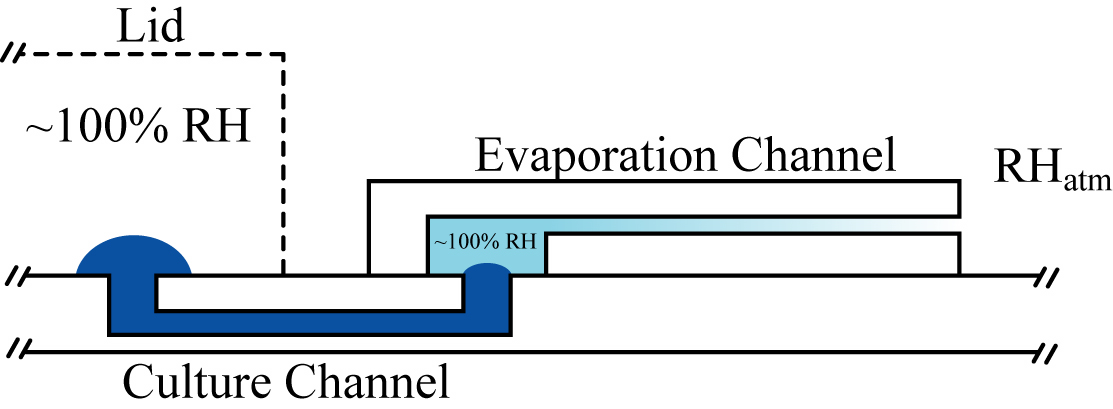
\includegraphics[width=4.5in]{EvaporationChannel.jpg}


\vspace{0.5cm}


b) 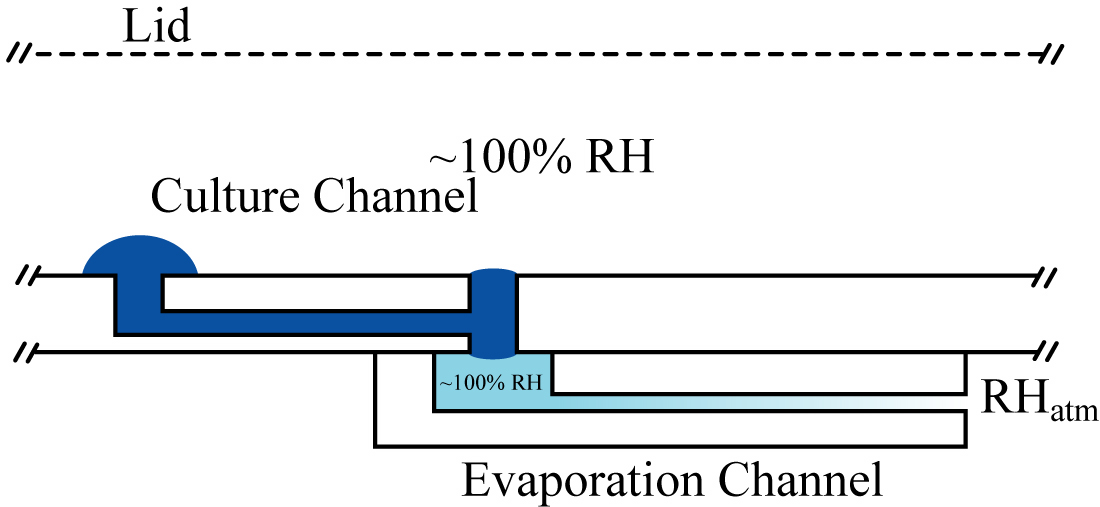
\includegraphics[width=4.5in]{EvaporationChannel2.jpg}
\caption{\textbf{Schematic representation of two different methods for controlling humidity to drive slow flow via evaporation}. The device design minimizes evaporation at non-evaporation ports (\ie , the port on the left) while the evaporation channel is an empty microchannel that resists evaporation at a rate proportional to the ratio of length to cross-sectional area. Varying the length of the evaporation channel linearly varies the evaporation rate and thus the flow through the device. a) Method 1 - Top-Side Evaporation Channel:  Both ports of the device are on the top-side of the substrate. b) Method 2 - Bottom-Side Evaporation Channel:  The evaporation channel is situated on the bottom-side of the substrate by creating a hole through the substrate. Preliminary results suggest the bottom-side design has advantages with respect to sterilization procedures, ease of use, and compatibility with PDMS and a material for making the microchannels.}
%Method 1) Two chamber design with variable sacrificial fluid. The inner chamber attempts to minimize evaporation from the non-evaporation ports while the exterior chamber controls evaporation through an appropriate amount and placement of sacrificial fluid (empirically determined) [CITE JAY/ERWIN].
\label{fig:evaporationDevices}
\end{figure}

The two designs implement the use of an evaporation vent. The evaporation vent is a microchannel that is left unfilled. One end of the channel has a port that encloses the evaporation port of the perfusion device. Vapor that is diffusing away from the evaporation port must diffuse through the evaporation vent. Therefore, the flux of vapor from the evaporation vent can be controlled by designing the cross-sectional area and length of the channel resist evaporation appropriately for the external humidity conditions. The resistance of the evaporation vent to vapor diffusion is proportional to the ratio of its length to its cross-sectional area. Silica beads will be used to control the external humidity at the underside of the device. 

%The major advantage using the evaporation vent is that the humidity external to the device does not need to be controlled such as with the use of a standard cell culture incubator. This makes the device much more portable and robust to external changes in humidity. If the evaporation vent is designed for dry external environments, then the device will better suited for the environments typical of microscopes or culture hoods, also it could eliminate the requirement for a humidified culture incubator. 

As this method is intended for use in cell culture, one obstacle to the implementation of an evaporation driven method for flow is the accumulation of solute near the evaporation port. Over the time-course of evaporation, increased osmolarity or high concentrations of toxic factors, if allowed to reach the culture region of the device, could adversely effect results. A diffusion valve that was developed in previous work with Erwin Berthier and used in previous work by lab members \cite{Frisk:2008pi} will be used to keep accumulation of solute from diffusing into regions used for cell culture. The diffusion valve is a microchannel with cross-sectional area to length ratio such that when a predetermined flow rate exists through the valve, solute, including small molecules such as ions, cannot diffuse significantly upstream. Thus, given two chambers connected by a diffusion valve, the upstream chamber is diffusionally isolated from the downstream chamber. 

Fig \ref{fig:pecletFlow} shows a plot of normalized concentration versus normalized length within the diffusion valve region given flows of various characteristic Peclet numbers. The Peclet number describes the balance between convective and diffusive transport given a fluid velocity, characteristic length, and diffusion coefficient (Pe = $L\,v/D$). The characteristic length that is appropriate for the diffusion valve is the valve length, as we are interested in transport along the length of the channel. Peclet numbers of ~3.0 suggest that, at stead-state, the upstream chamber is at 5\% the concentration of the downstream chamber. Some similar calculations include $\sim$4.6 $\rightarrow$ 1\%, $\sim$10 $\rightarrow$ 0.004\%, and $\sim$15 $\rightarrow$ 0.00003\%. It may seem extreme to look at such high values of the Peclet but many soluble factors can illicit cellular responses over many orders of magnitude of concentration. However, the calculations suggest that the upstream chamber can be effectively isolated from the downstream chambers.

A more detailed treatment of the diffusion valve including governing equations is contained in the Appendix.

\begin{figure}[!ht]
\centering
\includegraphics[width=3.5in]{DiffusionValve.pdf}
\caption{\textbf{Diffusion valve operation}. Plot of normalized concentration ratio (concentration at position $x/L$ divided by concentration at inlet of the downstream chamber) for various values of the Peclet number for the diffusion valve. $x/L=0$ is at the downstream chamber and $x/L=1$ is at the upstream chamber.}
\label{fig:pecletFlow}
\end{figure}

Another important consideration in the design of slow flow methods such as this is the range of appropriate flow rates for any attached culture chambers. The goal of future work is to create slow perfusion flow without significantly affecting the diffusive transport of factors locally within each culture chamber. Just as the diffusion analysis of Fig \ref{fig:pecletFlow} applies to the diffusion valve, it also applies to the culture chambers. Therefore, a desirable situation would be to keep the Peclet number below a value of 1 in the culture chamber, thereby attempting to minimize the gradient of factors that exist in the culture chamber. The diffusion valve is aimed at isolating small molecules while the culture chambers are aimed at evenly distributing large molecules. This disparity is accounted for in the designing of the relative lengths and widths of the culture chambers and diffusion valves. If the Peclet number is too high in the culture chamber, the cross-sectional area of the culture chamber can be increased or the chamber length can be reduced or, if it easier to modify the diffusion valve, the diffusion valve could be reduced in cross-sectional area or lengthened. These changes in dimensions allow the user to design chambers and valves to the particular flow or media exchange rate that is desired for culture chamber. Thus, fluid exchange rates can be adjusted to increase or decrease overall levels of accumulating factor and still maintain relatively even distributions of factor within the chamber.

The design parameters of the evaporation-based device are listed in Tab \ref{tab:evaporation}.

\begin{table}[!ht]
\centering
\begin{tabular}{ll} \toprule
Parameter & Decription \cr \midrule
$D_{d}$ & {\underline D}iffusion coefficient of solute of interest in the {\underline d}iffusion valve \cr
$D_{c}$ & {\underline D}iffusion coefficient of solute of interest in the {\underline c}ulture chamber \cr
$L_{d}$ & {\underline L}ength of the {\underline d}iffusion valve \cr
$L_{c}$ & {\underline L}ength of the {\underline c}ulture chamber \cr
$L_{e}$ & {\underline L}ength of the {\underline e}vaporation vent \cr
$A_{d}$ & Cross-sectional {\underline a}rea of the {\underline d}iffusion valve \cr
$A_{c}$ & Cross-sectional {\underline a}rea of the {\underline c}ulture chamber \cr
$A_{e}$ & Cross-sectional {\underline a}rea of the {\underline e}vaporation vent \cr
$RH$ & The {\underline r}elative {\underline h}umidity external to the device \cr \bottomrule
\end{tabular}
\caption{\textbf{Table of design parameters for evaporation mediated slow flow device}.}
\label{tab:evaporation}
\end{table}

\subsubsection{Surfactant Mediated Flow}\label{sec:deviceDesignSurf}
Just as surface tension plays the dominant role in producing flow via traditional \pp , surface tension can be modified to produce flow without any addition of fluid. In this device, surfactant is delivered to the output port of the device to cause a change in surface tension resulting in a pressure change that then causes flow in the perfusion device. Our chosen method of surfactant delivery is diffusion through a microchannel. Therefore, the time-scales of the flow are limited by diffusion and can be many hours, as dictated by the geometry of the delivery channel and reservoirs. The total volume pumped via this method is limited by the volumes of the input and output drop of the channel that is being influenced. The fluid velocity within the channel will be a result of the diffusion kinetics, the droplet sizes, and finally the channel geometry. One advantage of this design is that the volumes pumped are small and the fluid flow rate is limited by diffusion, therefore, very slow flow rates can be achieved in a controlled manner. A schematic of the device is shown in Fig \ref{fig:surfactantDevices}.

\begin{figure}[!ht]
\centering
\includegraphics[width=5in]{SurfactantFlowDiagram.pdf}
\caption{\textbf{Slow flow via surfactant diffusion}. Schematic representation of slow perfusion device mediated by controlled delivery of surfactants. Diffusion of surfactant reduces surface tension at the affected output drop. The reduced surface tension causes fluid to flow towards the affected output drop from other input ports in amounts related to the input port radii. Inputs with larger radii will be larger sources of flow. The diffusion valve can be designed to isolate the surfactant from upstream culture areas.}
\label{fig:surfactantDevices}
\end{figure}

The slow flow device shown in Fig \ref{fig:surfactantDevices}, is designed to validate the surfactant-based slow flow method and is not intended for culture. One or multiple culture chambers and their associated ports can be included upstream of the diffusion valve, which is in place to isolate surfactant from the culture components. As mentioned earlier, the diffusion valve is very effective at minimizing diffusion upstream for flows with a Peclet number significantly greater than 1. The output port is connected to a surfactant delivery channel and port. When very small volume of containing a high concentration of surfactant is placed at the surfactant delivery port, negligible flow will occur from \pp\ as the surfactant delivery port has a very small radius. The surfactant will then diffuse through the surfactant delivery channel to affect the output drop. Surfactant diffusing into the output drop will cause a reduction in surface tension and pressure. The loss of pressure causes flow towards the output drop, thereby producing flow for the diffusion valve to isolate surfactant from any upstream culture components.

%Specific dimensions were chosen via simulation of the device in Matlab using 1D simplified models of diffusion in the microchannel. The model assumes even mixing in the output port and a linear relationship between surfactant concentration and surface tension. The model was simulated for a range of surface tensions that would produce a $\sim$70\% reduction in surface tension at the output port (see Appendix). 

Initial simulations suggest that the diffusion process can be made to last hours or days with appropriate geometries. Over those time-courses, input and output volumes can be chosen to result in flow rates that would result in exchange of culture chamber media from fractions per day up to many times per day suggesting that it would be an appropriate method for slow perfusion microchannel culture.

Design parameters of the device, when used to perfuse fluid through a culture chamber are very similar to the evaporation based device with slight differences as shown in Tab \ref{tab:surfactant}.

\begin{table}[!ht]
\centering
\begin{tabular}{ll} \toprule
Parameter & Decription \cr \midrule
$D_{d}$ & {\underline D}iffusion coefficient of solute of interest in the {\underline d}iffusion valve \cr
$D_{c}$ & {\underline D}iffusion coefficient of solute of interest in the {\underline c}ulture chamber \cr
$D_{s}$ & {\underline D}iffusion coefficient of {\underline s}urfactant \cr
$L_{d}$ & {\underline L}ength of the {\underline d}iffusion valve \cr
$L_{c}$ & {\underline L}ength of the {\underline c}ulture chamber \cr
$L_{s}$ & {\underline L}ength of the {\underline s}urfactant delivery channel \cr
$A_{d}$ & Cross-sectional {\underline a}rea of the {\underline d}iffusion valve \cr
$A_{c}$ & Cross-sectional {\underline a}rea of the {\underline c}ulture chamber \cr
$A_{s}$ & Cross-sectional {\underline a}rea of the {\underline s}urfactant delivery channel \cr
$S$ & The type of {\underline s}urfactant delivered \cr \bottomrule
\end{tabular}
\caption{\textbf{Table of design parameters for surfactant mediated slow flow device}.}
\label{tab:surfactant}
\end{table}

One important unknown aspect of the design suggested by the parameter $S$ in Tab \ref{tab:surfactant} is the identity of the surfactant and the effectiveness of the surfactant to reduce surface tension in the media. A preliminary experiment will be performed using a goniometer to determine the surface tension profile of different concentrations of surfactant and media. The profile will influence the flow rate progression over time and will be important to evaluating the ability of this method to produce consistent flow over long intervals. One surfactant of interest is bovine serum albumin (BSA).

\subsection{Methods}

Methods common to many pieces of the work proposed here are described in the Appendix such as device manufacture and modeling of diffusion, signaling, and response.

\subsubsection{Device Characterization}
The device designs will be characterized by measuring total flow over time and observing the quasi-steady-state convection-diffusion of dye or fluorescently labeled molecules at different times. In the case of the evaporation-based slow flow device, flow will be measured as the total volume loss over time compared to a `no evaporation' control, whereas in the case of the surfactant mediated flow device, droplet profile will be measured at the input port to infer volume at various time-points and will also be compared to a `no evaporation' control.

\subsection{Preliminary Results} \label{sec:prelimCCResults}

Some preliminary testing has already been accomplished with respect to slow-perfusion via evaporation. However, the results were obtained in the context of work towards a `one-way co-culture' device and thus diagrams show devices that have two chambers instead of one as suggested in section \ref{sec:deviceDesignEvap}. Fig \ref{fig:oneWayDye}a shows images of a slow-perfusion device with two culture chambers. Each image shows a different scenario. The bright-field image is intended to show the shape of the device. The balloons labeled with the word `add' indicate that fluorescent dye was added to the chamber prior to flow. The images with the square chambers are simulation results false colored like the dye. In each case, the dye in the experiment and simulation are confined to be at or below the chamber to which it was added over the course of 24 hours. Thus, evaporation was successfully implemented to direct a slow flow that transports fluid at similar rates to diffusion in the culture chambers and the diffusion valves were effective barriers to diffusion upstream. The fluid velocity simulation diagram of Fig \ref{fig:oneWayDye} indicates the relative flow rates that exist in the diffusion valves versus the chambers.

\begin{figure}[!ht]
\begin{center}
\includegraphics[width=6.5in]{OneWay_Illustration_figure.png}
\caption{\textbf{Preliminary validation of real-time conditioned media assay device operation}. Microscope images demonstrating the function of the diffusion valve. Different dyes (Alexa488 and TexasRed bound to Dextran 10kD) were loaded in the chambers destined for cell culture and imaged after 24 hours. The profiles show the presence of dyes downstream of diffusion valves but not upstream. COMSOL simulations were performed by supposing constant production of dye in the chamber after 20 hours. The velocity fields obtained are displayed.}
\label{fig:oneWayDye}
\end{center}
\end{figure}

\subsection{Expected Challenges}
Preliminary results suggest that there will be some challenges with respect to the technical implementation. One of the evaporation designs requires cutting through the polystyrene substrate, which can be a challenge. However, we have just purchased a CO$_{2}$ laser cutting system which has the capability to cut holes through polystyrene with sufficient accuracy. Processing parameters for optimal hole manufacture are still undetermined but is the focus of a hired undergraduate over the semester.

Further, the evaporation device that requires laser cutting will also need a method to create a dry environment on the bottom side of the device. Preliminary tests have shown that we can either use a sealed lid and a dry incubator or a non-sealed lid and a sealed chamber under the channel in which humidity is depleted using silica beads. The latter appears to have the most advantages as it allows for a more free gas exchange with the gas controlled incubator. However, the capacity of the silica beads to maintain a dry environment has not been thoroughly investigated but first indications are that they are quite sufficient.

\paragraph{Side note for future work:}Just as silica beads can be used to create an atmosphere depleted of water vapor at the underside of the evaporation device, other materials exist that can deplete or supply other gaseous molecules such as oxygen. In this way, different concentrations of gaseous molecules could be maintained at each end of a microchannel to create gradients. The work proposed here represents a first step towards such gradient devices that could be a way to readily examine the effects of microenvironmental parameters such as oxygen tension.

\section{Cross Flow in the Diffusion Region}
The following fluidic device can be analyzed using an electrical analogy (see Fig \ref{App:PerfusionCulture:fig:device}). The electric circuit analogy can be split into an analogous circuit in which there are two voltage sources. Now the problem can be solved using superposition. When using superposition, one voltage source is disconnected and the circuit is solved. The same is done using the other as the sole voltage source. This solutions are then added to obtain total voltages and currents which should match the results of the original circuit. 

\begin{figure}[!ht]
\centering
a) \includegraphics[height=2in]{Device.pdf}     b) \includegraphics[height=2in]{Original.pdf}
\caption{\textbf{Perfusion co-culture}. Perfusion co-culture device in which flow ratios will be estimated and its electric circuit analog.}
\label{App:PerfusionCulture:fig:device}
\end{figure}

Fig \ref{fig:circuit} shows two circuits, that when solved and their solutions added together, give the solution to the original circuit shown in Fig \ref{App:PerfusionCulture:fig:device}.

\begin{figure}[!ht]
\centering
\includegraphics[height=2in]{Analog.pdf}
\caption{\textbf{Perfusion co-culture circuit analog}. Diagrams of circuits that when added together, are equivalent to the original circuit of Fig \ref{App:PerfusionCulture:fig:device}. The circuits shown here are easier to solve and are used in the math that follows to find the ratios of currents or fluid flows through the device as compared to the total flow through the device.}
\label{fig:circuit}
\end{figure}

The left-hand and right-hand circuit have the following equivalent resistances.

\begin{equation}
R_{LH} = R_{1} + \frac{1}{\frac{1}{R_{4}} + \frac{1}{C_{LH}}}\textrm{, where } C_{LH} = R_{3} + \frac{1}{\frac{1}{R_{5}} + \frac{1}{R_{2}}}
\end{equation}
\begin{equation}
R_{RH} = R_{2} + \frac{1}{\frac{1}{R_{5}} + \frac{1}{C_{RH}}} \textrm{, where } C_{RH} = R_{3} + \frac{1}{\frac{1}{R_{4}} + \frac{1}{R_{1}}}
\end{equation}

Therefore the ratio $I_{1}/I_{2}$ is equal to the ratio $R_{RH}/R_{LH}$. Now if we solve for $I_{3}$ in each circuit, we can use the information to indicate the proporation of total current through the circuit that is devoted to pass through $R_{3}$ (\ie , the fluid flow through the diffusion valve).

In the left-hand circuit, 
\begin{equation}
I_{2}^{LH} =\frac{V}{R_{LH}}
\end{equation}
\begin{equation}
I_{3}^{LH} =\frac{I_{1}^{LH}}{1+ \frac{C_{LH}}{R4}}
\label{equ:LHI3}
\end{equation}
\begin{equation}
I_{2}^{LH} =\frac{I_{3}^{LH}}{1+\frac{R_{2}}{R_{5}}}
\end{equation}
and in the right-hand circuit
\begin{equation}
I_{1}^{RH} =\frac{V}{R_{RH}}
\end{equation}
\begin{equation}
I_{3}^{RH} =\frac{I_{1}^{RH}}{1+ \frac{C_{RH}}{R5}}
\label{equ:LHI3b}
\end{equation}
\begin{equation}
I_{1}^{RH} =\frac{I_{3}^{RH}}{1+\frac{R_{1}}{R_{4}}}
\end{equation}
and by superposition,
\begin{equation}
I_{3} = I_{3}^{LH} - I_{3}^{RH}
\label{equ:I3}
\end{equation}
\begin{equation}
I_{1} = I_{1}^{LH} - I_{1}^{RH}
\label{equ:I1}
\end{equation}
\begin{equation}
I_{2} = I_{2}^{RH} - I_{2}^{LH}
\label{equ:I2}
\end{equation}

The minus sign is to indicate that the $I_{1}$, $I_{2}$, and $I_{3}$ currents are in opposite directions in the RH and LH circuits. This then allows us to write the proportion of total current that flows through the diffusion region as the following.

\begin{equation}
\textrm{Cross Flow Ratio} = \frac{I_{3, tot}}{I_{1} + I_{2}}
\end{equation}

Using the above equations Fig \ref{fig:crossFlow} was created to observe the influence of unbalanced resistance on the rate of cross flow through the bridge relative to the total flow through the device. This is done by varying only the resistance of $R_{5}$.

\begin{figure}[!ht]
\centering
\includegraphics[width=3.5in]{CrossFlowPlot.pdf}
\caption{\textbf{Cross-flow during perfusion co-culture}. Calculations of relative cross flow rate using electrical analog equations for different output resistance ratios.}
\label{fig:crossFlow}
\end{figure}

\section{Peclet Ratio}

Diffusive flux in a rectangular duct with 1D diffusion is proportional to the following expression, $J \propto D\,A/L$ where $D$ is the diffusion coefficient describing the solvent and solute, $A$ is the cross-sectional area of the duct, and $L$ is the length of the duct. Therefore, to maximize the flux through the diffusion region we would like to maximize $A$ and minimize $L$.

In order to maximize diffusive flux in the parallel perfusion co-culture device the diffusion region length, $h_{d}$, will likely be the same height as the culture region, $h_{c}$, and the length roughly 1/10$^{th}$ the culture chamber length (\ie , $h_{d}/h_{c} \approx 1$, and $L_{d}/L_{c} \approx 0.1$). A significant width for the diffusion region might also be roughly the width of the culture chambers (\ie , $w_{d}/w_{c} \approx 1$).

The Peclet number of a flow is given by $Pe = L\,v/D$ which can also be written in terms of the flow rate for a duct as $Pe = L\, Q \, w \, h/D$. Further, if we estimate the flow rate in each culture chamber as being half of the total flow for a reasonably balanced system, we can write an expression for the ratio of Peclet numbers for the culture chambers versus the diffusion region between the chambers ($Pe_{c}/Pe_{d}$, culture chamber over diffusion region).

\begin{equation}
Pe_{c}/Pe_{d} = \frac{L_{c}Q_{c}w_{c}h_{c}}{L_{d}Q_{d}w_{d}h_{d}}
\end{equation}

Using conclusions from the previous section and assuming the flow in each culture chamber is about half of the total flow through the device, we can estimate the flow rate ratios, $Q_{c}/Q_{d} \approx 0.04$. We have already suggested that $h_{c}/h_{d} \approx 1$, $w_{d}/w_{c} \approx 1$, and $L_{c}/L_{d} \approx 0.1$. Therefore, it is expected that the ratio of the diffusion region Peclet number and culture chamber peclet number will be roughly $0.04 \times 1 \times 1 \times 0.1 \approx 0.004$. Since the aim of the coculture device is to keep the Peclet number in the culture chamber close to 1, the Peclet number in the diffusion region will be $\ll 1$ ensuring relatively unbiased communication between the two chambers.


%Now if we assume the following,
%\begin{equation}
%R1/R2 = \alpha
%\end{equation}
%\begin{equation}
%R4/R5 = \beta
%\end{equation}
%then each of the above equations can be collapsed to the following.

%\begin{equation}
%R_{LH} = \alpha R_{2} + \frac{1}{\frac{1}{\beta R_{5}} + \frac{1}{C_{LH}}}\textrm{, where } C_{LH} = R_{3} + \frac{1}{\frac{1}{R_{5}} + \frac{1}{R_{2}}}
%\end{equation}
%\begin{equation}
%R_{RH} = R_{2} + \frac{1}{\frac{1}{R_{5}} + \frac{1}{C_{RH}}} \textrm{, where } C_{RH} = R_{3} + \frac{1}{\frac{1}{\beta R_{5}} + \frac{1}{\alpha R_{2}}}
%\end{equation}



%		Clh = (R3 + (1/((1/R5) + (1/R2))));
%		System.out.println("Clh: " + Clh);
%		Crh = (R3 + (1/((1/R4) + (1/R1))));
%		System.out.println("Crh: " + Crh);
%		
%		Rlh = R1 + 1/((1/R4) + (1/Clh));
%		System.out.println("Rlh: " + Rlh);
%		Rrh = R2 + 1/((1/R5) + (1/Crh));
%		System.out.println("Rrh: " + Rrh);
%		
%		I1lh = 1/Rlh;
%		System.out.println("I1lh: " + I1lh);
%		I3lh = I1lh/(1+(Clh/R4));
%		System.out.println("I3lh: " + I3lh);
%		I2lh = I3lh/(1+(R2/R5));
%		System.out.println("I2lh: " + I2lh);
%		
%		I2rh = 1/Rrh;
%		System.out.println("I2rh: " + I2rh);
%		I3rh = I2rh/(1+(Crh/R5));
%		System.out.println("I3rh: " + I3rh);
%		I1rh = I3rh/(1+(R1/R4));
%		System.out.println("I1rh: " + I1rh);










% \bibliographystyle{abbrvnat}
% \begin{singlespacing}
% \bibliography{./Bibliography/bib}
% \bibliography{library1.bib}
% \end{singlespacing}

\printbibliography

\end{document}






















































































